%%%%%%%%%%%%%%%%%%%%%%%%%%%%%%%%%
% 6CCS3PRJ Final Year Individual Project Report
% luca-dorin.anton@kcl.ac.uk
%%%%%%%%%%%%%%%%%%%%%%%%%%%%%%%%%
\documentclass[11pt]{informatics-report}
\usepackage{color}
\usepackage[square,sort,comma,numbers]{natbib} %References
\usepackage{hyperref}
\usepackage{graphicx}
\usepackage{float}
\usepackage{pdfpages}
\usepackage{listings}
\graphicspath{ {./Images/} }

%%%%%%%%%%%%%%%%%%%%%%%%%%%%%%%%%
% Front Matter - project title, name, supervisor name and date
%%%%%%%%%%%%%%%%%%%%%%%%%%%%%%%%%
\title{Design and Implementation of a 16-bit Breadboard Computer Architecture\\\vspace{0.2cm}6CCS3PRJ - Individual Project Report}
\author{Luca-Dorin Anton}
\studentID{1710700}
\supervisor{\textbf{Dr. Christian Urban}}

\date{\today}

\abstractFile{FrontMatter/abstract.tex}
\ackFile{FrontMatter/acknowledgements.tex} %Remove line if you do not want acknowledgements

\begin{document}
\createFrontMatter
\onehalfspacing
\tableofcontents
\doublespacing

%%%%%%%%%%%%%%%%%%%%%%%%%%%%%%%%%
% Report Content
%%%%%%%%%%%%%%%%%%%%%%%%%%%%%%%%%
% You can write each chapter directly here or in a separate .tex file and use the include command.

\chapter{Introduction}
As the demand for high speed, low power, efficient and cheap computers rose over the past three decades,
manufacturers invested heavily into improving production processes, shrinking transistors, pipelining
instructions, creating new aggressive branch prediction models and implementing more and more functionality
into the hardware directly. Moore's prediction on the number of electronic components doubling on the
same surface area every two years held up well until recently when issues of quantum tunnelling started to
arise. This hasn't stopped the continuous enhancement of microprocessor and microsystems though. Now, instead
of making components smaller, manufacturers are installing more processing cores onto a single computing chip
package.
\begin{figure}[ht]
  \centering
  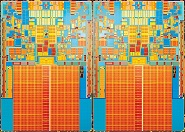
\includegraphics{45nm_quad_core_die}
  \caption{Intel quad-core 45nm CPU die}
  \label{intel_die}
\end{figure}
\linebreak
Another way of improving hardware is by implementing complex functionality, which would have been achieved traditionally through software, directly in hardware. An example of this is the implementation of the \emph{Advanced Encryption Standard} (AES) by \emph{Intel} directly in their lineup of CPUs through the \emph{AES-NI} instruction set extension \cite{aes2012ni}.
While the advantages for modern society of the continuous and accelerated development of hardware cannot be doubted,
there are also some worrying disadvantages. Such an advanced level of complexity in microprocessor design has been reached, that system and chip designers have started to increasingly rely on abstraction tools like \emph{ High-Level Synesthesis} to accommodate the advanced design requirements and meet user needs, as noted by Coussy in the \emph{User Needs} chapter \cite{coussy2008high}. On the one hand, this increasing complexity of hardware poses challenges for operating system and compiler developers, who need to constantly stay up to date with the newest improvements in the hardware space and integrate them into their products, to ensure user satisfaction and sustained quality over time. One the other hand, people, including developers, are presented with no need to understand the underlying machines with which they are interacting. To quote Bruce Scheiner, a famous cryptographer and computer scientist:
\begin{quotation}
People don't understand computers. Computers are magical boxes that do things. People believe what computers tell them. \cite{schneier2011secrets}
\end{quotation}
As a possible solution to this general human trend towards treating computers as ~~magical boxes'', this project proposes a simple and understandable \emph{practically implementable} machine architecture which has the same computational capabilities as a Turing machine. \linebreak
Some core features of the architecture are:
{\begin{itemize}
  \item 16-bit word length
  \item variable clock speed for live execution visualization
  \item single clock step function
  \item simplified input and output
  \item hardware addition and subtraction implementation
\end{itemize}}

The rest of the report will go through the steps involved in specifying, designing, building and testing the machine and the software to go along with it in great detail.
\pagebreak
\section{Inspiration and Motivation}
The main inspiration for this project is a YouTube series created by \emph{Ben Eater} titled \emph{~~Building an 8-bit breadboard computer!''} \cite{eater2019breadboard}. Eater's computer is itself a physical implementation of a theoretical
architecture called \emph{SAP-1}, which stands for \emph{Simple as Possible}. There are three variants of the SAP Architecture, SAP-1, SAP-2 and SAP-3, in inreasing order of complexity, all of which have been created by Malvino and Brown in their book \emph{Digital computer electronics} \cite{malvino1992digital}.
\begin{figure}[ht]
  \centering
  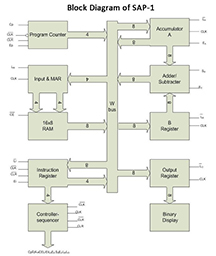
\includegraphics{sap1}
  \caption{Block Diagram of the SAP-1 architecture}
  \label{sap1}
\end{figure}
\linebreak
After going through the content, it became apparent that such a computer could serve as a great learning medium for developing a better understanding of computers, even more so with some hardware improvements and a sizable effort in writing some bespoke software for it. \emph{This project is largely based around Eater's design.} It serves not only as the motivational source for the project, but it also provides a solid foundation for which extension, enhancement and improvement can be within the scope of a final year project.

\section{Objectives}
The main goal of this project is the physical implementation of a 16-bit computer system modelled after an architecture designed around the ideas of \emph{explainability and ease of understanding} down to the transistor level. Breaking down this objective by specific hardware and software requirements, the following can be stated:
The main anaysis goals are:
\begin{enumerate}
  \item Detailed analysis of computer architecture
  \item Analysis of the computer designed and built by Ben Eater \cite{eater2019breadboard}
\end{enumerate}

The main hardware  objectives are:
\begin{enumerate}
  \item 16 bit word length
  \item appropiatley sized memory space
  \item memory read/write capability
  \item capability to decode and execute instructions sequentially
  \item program counter alteration (jumps)
  \item I/O functionality
  \item hardware-implemented ability to perform basic arithmetical operations \label{aritm}
  \item simple branching
  \item variable speed clock
  \item single step clock function
\end{enumerate}
\pagebreak
The main software objectives are:
\begin{enumerate}
  \item microcode generation tool
  \item adequate microcode for the control mechanisms
  \item assembly mnemonics
  \item assembler package to turn assembly files into binaries
  \item compiler for the WHILE-language to breadboard computer binaries
  \item Arduino driver software
\end{enumerate}

\section{Project Structure}
The report begins with an in-depth circuit specification, design and analysis literature review. These core skills lay the theoretical foundation necessary for understanding the reasoning for choices when designing the hardware.
The next section is concerned with a detailed analysis of the computer built by Ben Eater \cite{eater2019breadboard}. Eater's computer serves as the template from which the design of the computer described in this report will originate. As such, it makes sense to analyse it carefully and classify its capabilities. \\
This will be followed by a specification of what the new computer should achieve in contrast to the capabilities of the existing computer. \\
The next chapter will cover the updated design of the computer. Important design decisions will be scrutinised and held against the main goals of the project. Both high-level, as well as in-depth design choices, will be taken into account. Main design challenges will be discussed and appropriate solutions presented. \\
After the design stage is complete, the following chapter will document the implementation phase. A detailed chronological breakdown of build progress will be presented. Testing will be executed in parallel with the implementation. \\
With the implementation phase complete, the software development phase will follow. The design and implementation of the various software tools necessary for running the breadboard computer will be documented in this chapter.
With the software as well as the hardware ready, a rigorous testing phase will follow, coupled with an in-depth evaluation of the end product in comparison to the success criteria set at the start of the report. \\
Finally, the conclusion chapter summarises everything done so far and highlights the learning outcomes of the project and the possible continuation paths for future work. \\

\chapter{Background}
Since this project is largely focused around designing and building a new hardware architecture,
it is necessary to go through the existing material surrounding this topic. Hardware design can
be structured in many different ways. For the purposes of this report, a structuring based on increasing
abstraction levels will be used. Since the implementation objectives of the project aim to be educational in nature,
it is crucial to start off with as few assumptions about the existing systems as possible. As such, the following explanations assume zero previous knowledge. Besides this, the educational outcomes largely focus on developers and computer scientists, professionals who would benefit from a better understanding of the computer but who are not necessarily familiar with the field of logic design. As such, the definitions and explanations will be kept as brief as possible, to avoid possibly superfluous levels of detail.

\section{Computer Architecture}
Computer architecture refers to organization, functionality and implementation design details of a computer system. It can be generally split into two main categories: \emph{Instruction Set Architecture} and \emph{Microarchitecture}.

\subsection{Instruction Set Architecture (ISA)}
The \emph{Instruction Set} is the set of unique operations the computer is capable of performing. It is generally independent of the physical implementation of the system and it serves as an interface against which assembler, compiler and operating system designers and engineers can structure their products. ISA design will be a crucial part of this project. By building a hardware architecture from scratch, the opportunity for many different ISA design choices will present itself. Many of those choices will be presented, implemented and analysed in this report.

\subsection{Microarchitecture}
A computing system's microarchitecture refers to concrete and detailed implementation choices for the hardware which is to implement the Instruction Set defined through the ISA. For the purposes of this project, the microarchitecture design will come first, which will be done against a general set of requirements and then the ISA design will follow based on the hardware design choices made. The ISA design will serve as a stepping stone towards the software architecture stage of the project.

\subsection{General High-Level Architecture}
Generally speaking, all computers share some high-level design features:
\begin{itemize}
  \item \emph{A Processor,} or \emph{Arithmetic-Logic Unit (ALU),} which performs operations on some data
  \item \emph{A Memory} or \emph{Storage Unit,} which stores both data and instructions
  \item \emph{A Control Unit,} which decodes instructions and issues control signals
  \item \emph{Input/Output (I/O) devices,} to communicate with the outside world
  \item \emph{A Clock Pulse Generator,} which keeps all other modules running synchronously
  \item \emph{A Data Bus,} to facilitate the transfer of information between modules
\end{itemize}
Each individual component will be discussed in great detail in this report.

\begin{figure}[H]
  \centering
  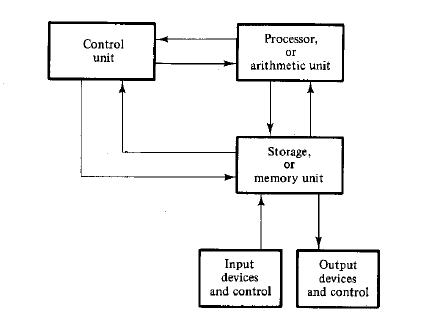
\includegraphics{comp_architecture}
  \caption{Block diagram of a digital computer, adapted from \emph{Digital Logic and Computer Design} by M. Morris Mano \cite{mano2017digital}}
  \label{comp_architecture}
\end{figure}

Figure \ref{comp_architecture} is a block diagram based on the previous listing of modules. The Data Bus is represented as the double-ended arrows connecting the different components together. The clock is omitted.

\subsection{The Processor}
The processor module is tasked with executing certain operations on data. Its mode of operation is only dependent on two inputs: the data to be operated on and the operation to be applied to that data. As such, the processor does not have to hold any kind of internal state; its output will always be the same for a certain input. This makes the processor a \emph{cobinatorial circuit}, meaning that it just implements some (albeit complex) logic function and does not have any internal state or memory.

\subsection{Memory}
Memory serves the purpose of storing data and instructions and returning the stored information when requested. By nature, it is a \emph{sequential} circuit, meaning that it has some internal state besides the logical function implementations used to communicate with the rest of the computer. Memory is organized in addresses, each address storing a word of information.

\subsection{The Control Unit}
The Control Unit oversees all other modules and ensures that everything is happening according to the present instruction. It also has the task of decoding the present instruction to correctly select the control signals which have to be issued next.
There are two main design choices to be made when constructing a Control Unit. One option is to \emph{hardwire} the logic. Whilst more efficient, this often proves to be tedious and very hard to alter. Another common and more accessible approach is the use of \emph{microcode.} Microcode control units use some sort of \emph{Read-Only Memory (ROM)} as a \emph{lookup table} to decide which control signals to switch on at a given time step of a given instruction. This lookup table is microcode. As it is implemented through a ROM, it can be easily reprogrammed or swapped out for a different ROM, making the maintenance of the Control Unit much more accessible.

\subsection{Input/Output Devices}
Input devices are used to inject instructions and data into the computer. Output devices communicate calculated results back to the user. I/O devices can take many forms and usually also require the computer to implement some sort of \emph{interrupt} system to notify the control logic that an external event is taking place. In the case of the computer built for this project, I/O devices will be abstracted as simple registers. The computer will read from and write to those registers.

\subsection{The Clock Pulse Generator}
Computers rely on a master clock to synchronise the activity of all other components. In modern microcomputers, this is usually accomplished through a \emph{crystal osscilator} which vibrates at a predetermined frequency. There are also other ways to achieve a steadily pulsating clock signal. In the case of the computer built in this report, a pair of voltage comparators will be used.

\subsection{The Data Bus}
Given a large number of modules present in a computer, it comes off as impractical to have each module communicate with each other module directly. In this situation, the data bus presents itself as an adequate solution. All modules connect both their input and their output terminals to the bus through some guard or buffer which allows them to disconnect from the bus as needed. Then, at any given clock pulse, only one device is allowed to connect and output to the bus, whilst any devices interested in receiving that information can connect and input from the bus. As long as only one device writes to the bus per clock cycle, the bus functions properly.

\subsection{Other Important Components}
Besides the main modules listed above, there are a few more components which are crucial to the optimal operation of a computer.

\subsubsection{Registers}
Registers are small memory units which can store only one word of memory. A computer system normally has a very limited amount of registers. In modern computers, registers have much shorter access times than memory. Besides storing data and programs, registers can have special functions, for example, input and output registers, registers tied to certain operations, flags registers and instruction registers.

\subsubsection{Power Supply}
Since the focus of this project is electrical computers, some sort of electrical power supply will be necessary. A simple solution for a power supply based on a mobile phone charger will be presented in a later section of the report.

\section{Implementing individual modules}
With the general architecture of a computer system in place, the next design step is to create and implement design for each individual module. This can be achieved by using circuit design theory and best practices.

\subsection{Types of electrical circuits}
Electrical circuits can be broadly classified into two main categories: \emph{combinatorial} and \emph{sequential} circuits. \emph{Combinatorial circuits} are circuits without any internal state (no memory) which implement a certain logic function. A logic function maps binary inputs to binary outputs. They are implemented as cascading layers of \emph{logic gates.} The main techniques which can be used to transform a logic function into a combinatorial circuit are standard form reductions, map creations and adequate use of don't care conditions (input/output conditions which are considered to be invalid/ will never happen). \emph{Sequential circuits} are composed of two parts:
\begin{enumerate}
  \item A memory structure usually built out of \emph{flip flops}
  \item One ore more combinatorial circuits, implementing some logical functions
\end{enumerate}

\subsection{Logic Gates}
Logic gates are electronic devices usually built out of transistors which perform certain logic functions.
A \emph{logic function} is a function which maps binary inputs to binary outputs.

\subsection{The Transistor}
A transistor is an electronic device which allows the control of the flow of one current source through a second, potentially smaller current source. This serves as the basic component for creating more advanced electronic components like logic gates.
\begin{figure}[h]
  \centering
  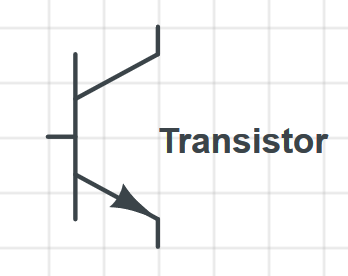
\includegraphics{trans}
  \caption{Transistor Symbol}
  \label{trans}
\end{figure}
Today, the most popular type of transistor and the most widley produced device in the world is the MOSFET \cite{chm2019mosfet}.


\subsection{Buffers}
Buffers are simple logic gates which just pass through the signal they receive.
\begin{table}[H]
\centering
\begin{tabular}{l|l}
\hline
\multicolumn{1}{|l|}{\textbf{A}} & \multicolumn{1}{l|}{\textbf{B}} \\ \hline
0                                & 0                               \\
1                                & 1
\end{tabular}
\caption{Truth table of a buffer}
\label{tab:buffer-table}
\end{table}
TO DO: ADD CIRCUIT DIAGRAM

\subsection{Inverters}
Inverters are similar in complexity to buffers. They invert the signal they receive.
\begin{table}[H]
\centering
\begin{tabular}{l|l}
\hline
\multicolumn{1}{|l|}{\textbf{A}} & \multicolumn{1}{l|}{\textbf{B}} \\ \hline
0                                & 1                               \\
1                                & 0
\end{tabular}
\caption{Truth table of an inverter}
\label{tab:inverter-table}
\end{table}
TO DO: ADD CIRCUIT DIAGRAM

\subsection{AND Gates}
And gates output a logic 1 only if all of their inputs are logic 1's.
\begin{table}[H]
\centering
\begin{tabular}{l|l|l}
\hline
\multicolumn{1}{|l|}{\textbf{A}} & \textbf{B} & \multicolumn{1}{l|}{\textbf{O}} \\ \hline
0                                & 0          & 0                               \\
1                                & 0          & 0                               \\
0                                & 1          & 0                               \\
1                                & 1          & 1
\end{tabular}
\caption{AND Gate Truth Table}
\label{tab:and-table}
\end{table}
TO DO: ADD CIRCUIT DIAGRAM

\subsection{OR Gates}
OR gates output a logic 1 if either of their inputs or both of them are logic 1's.
\begin{table}[H]
\centering
\begin{tabular}{l|l|l}
\hline
\multicolumn{1}{|l|}{\textbf{A}} & \textbf{B} & \multicolumn{1}{l|}{\textbf{O}} \\ \hline
0                                & 0          & 0                               \\
1                                & 0          & 1                               \\
0                                & 1          & 1                               \\
1                                & 1          & 1
\end{tabular}
\caption{OR Gate Truth Table}
\label{tab:or-table}
\end{table}
TO DO: ADD CIRCUIT DIAGRAM

\subsection{XOR Gates}
Exclusive OR, or XOR gates output a logic 1 only if either of their inputs is a 1, but not both.
\begin{table}[H]
\centering
\begin{tabular}{l|l|l}
\hline
\multicolumn{1}{|l|}{\textbf{A}} & \textbf{B} & \multicolumn{1}{l|}{\textbf{O}} \\ \hline
0                                & 0          & 0                               \\
1                                & 0          & 1                               \\
0                                & 1          & 1                               \\
1                                & 1          & 0
\end{tabular}
\caption{XOR Gate Truth Table}
\label{tab:xor-table}
\end{table}
TO DO: ADD CIRCUIT DIAGRAM

\subsection{NAND Gates}
A NAND gate is an inverted AND gate. This means it outputs a logic 1 in all situations except for when all of its inputs are logic 1's.
\begin{table}[H]
\centering
\begin{tabular}{l|l|l}
\hline
\multicolumn{1}{|l|}{\textbf{A}} & \textbf{B} & \multicolumn{1}{l|}{\textbf{O}} \\ \hline
0                                & 0          & 1                               \\
1                                & 0          & 1                               \\
0                                & 1          & 1                               \\
1                                & 1          & 0
\end{tabular}
\caption{NAND Gate Truth Table}
\label{tab:nand-table}
\end{table}
TO DO: ADD CIRCUIT DIAGRAM


\subsection{NOR Gates}
A NOR Gate is an inverted OR gate. This means it outputs a logic 1 only if all of its inputs are logic 0's.
NAND and NOR gates are considered \emph{universal gates}. This means that any logic circuit can be built exclusivley out of NAND or out of NOR gates.
\begin{table}[H]
\centering
\begin{tabular}{l|l|l}
\hline
\multicolumn{1}{|l|}{\textbf{A}} & \textbf{B} & \multicolumn{1}{l|}{\textbf{O}} \\ \hline
0                                & 0          & 1                               \\
1                                & 0          & 0                               \\
0                                & 1          & 0                               \\
1                                & 1          & 0
\end{tabular}
\caption{NOR Gate Truth Table}
\label{tab:nor-table}
\end{table}
TO DO: ADD CIRCUIT DIAGRAM

\subsection{Flip Flops}
Flip Flops are circuits usually built out of logic gates which can store one bit of information, i.e. they can be either on or off. There are many types of flip flops: RS-flip-flops (Reset-Set), D-flip-flops (Data), JK-flip flops (refined RS flip flops) and T flops (single input JK flip-flops). Each flip flop performs best in a certain scenario. Since they all implement de storage and retrieval of one bit of information, only the D-flip-flop (the most commonly used one) will be discussed. \\
TODO: ADD D FLIP FLOP DESC.


\section{8-Bit Computer Architecture Designed by Ben Eater \cite{eater2019breadboard}}
This section concerns itself with the detailed analysis of the 8-bit computer architecture designed by Ben Eater in his YouTube tutorial series \cite{eater2019breadboard}. This computer serves as the starting design for the computer discussed in this report in the later section, as such, it presents itself as a good topic for discussion.

\subsection{Main Features}
The main features of Bean Eater's 8-bit computer on a breadboard can be broken down as follows:
\begin{enumerate}
  \item 16 by 8 memory space (4-bit addresses, 8-bit words)
  \item adjustable and manually single-steppable clock
  \item two data registers: A and B
  \item ALU which implements addition, subtraction and simple branching based on zero and carry conditions
  \item Decimal output through three 7-segment displays
  \item Microcode-based control logic using \emph{EEPROMs} (electronically erasable and programmable read-only memory)
  \item Common 8-bit data and instruction bus
\end{enumerate}

\subsection{High-Level Overview}
\begin{figure}[ht]
  \centering
  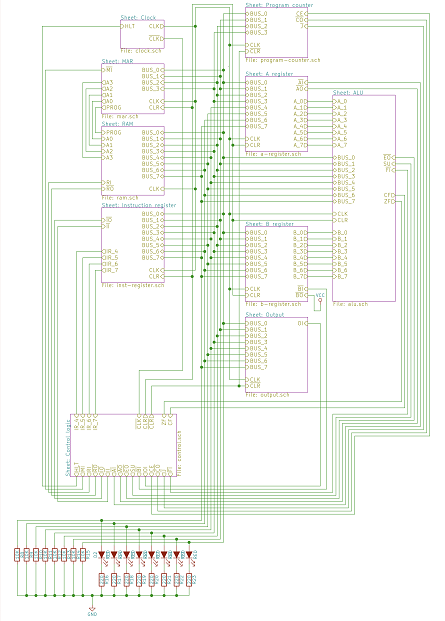
\includegraphics{8-bit-high-level}
  \caption{Block diagram of the 8-bit computer built by Ben Eater \cite{eater2019highlevel}}
  \label{8-bit-high-level}
\end{figure}



Figure \ref{8-bit-high-level} is a high-level block diagram displaying the inner workings of the 8-bit computer built by Ben Eater\cite{eater2019breadboard}. The following observations can be made when observing this diagram:
\begin{enumerate}
  \item Each module is connected directly to the common data bus. This means that every module can output information to the bus each clock cycle. After a judicious inspection of the microcode\cite{eater2019microcode} it is clear that no two modules output to the bus at the same time.
  \item The clock signal and the inverse clock signal are distributed throughout the computer to each module. Also, notice how there is a control signal for the clock as well. This \emph{HLT} (Halt) signal allows the computer to halt the clock, and implicitly halt the execution, for example after finishing a calculation, to allow it to be displayed.
  \item Besides the main connections through the bus, there are some additional \emph{special connections} between certain modules. For example, the \emph{A register} and the \emph{B register} have a direct connection to the \emph{ALU}, the \emph{MAR} (Memory address register) has a direct connection to the \emph{RAM} (Random Access Memory) and the \emph{IR} (Instruction Register) has a direct connection to the control logic.
  \item All control signals originate from the \emph{Control Logic} and spread out throughout the computer. Each module has at least one control signal
  \item This computer is severely limited in terms of memory. While 16 bytes can be sufficient for some demonstrational trivial programs (like Factorial or Fibonacci), it is insufficient for anything else.
  \item Another major limitation is the fact that it can only operate on signed integers. The architecture represents data in \emph{big endian, two's complement integer} format. No other data format or type is supported.
\end{enumerate}

\subsection{Module Design Conventions}
Ben Eater follows some essential design conventions when designing and building each of the modules for his computer.
The following subsections describe those conventions.

\subsubsection{Simplicity of understanding over cost and efficiency}

In many situations where a simpler solution from cost or efficiency makes itself notices, Eater often chooses to go for a more pragmatical approach which focuses on the simplicity of understanding. Since his computer mostly serves as an educational tool, it makes sense to pursue solutions which are easy to understand, over solutions which might be slightly cheaper or more efficient. A good example of this is in the design of the clock module \ref{eater2019clock}.

\begin{figure}[ht]
  \centering
  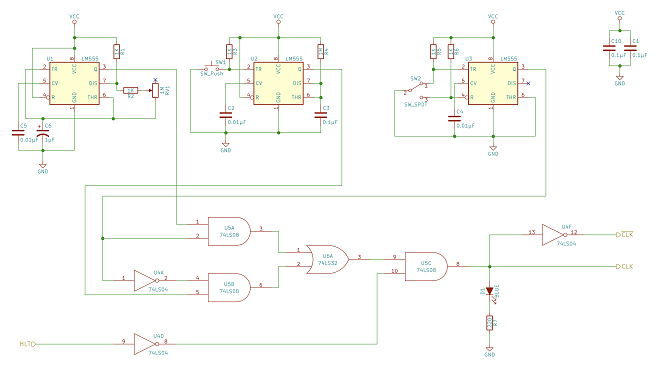
\includegraphics{8-bit-clock}
  \caption{Schematic of the clock module in Bean Eater's 8-bit computer \cite{eater2019highlevel}}
  \label{8-bit-clock}
\end{figure}

For the combinatorial circuit responsible for selecting a clock signal (either the automatic or the manual one) and also filtering out the clock when the \emph{HLT} (Halt) signal is active, Eater could have opted for a circuit built out of \emph{NAND} (Not And) gates instead of a circuit of AND, OR and inverter gates. This is because NAND gates are universal gates, which means that any combinatorial circuit can be built exclusively out of NAND gates. In this case, this would have had a net effect on cost, since the circuit could have been implemented with only two NAND ICs (integrated circuits), instead of three. The choice was made to use AND, OR and Inverter gates since the function of those gates is more intuitive and as such, the entire circuit is easier to understand.

\subsubsection{Connection to the Bus}

Eater's computer features an 8-bit common bus for both data and instructions. Most modules are tied to this bus directly. For the bus to function properly, only one device should be allowed to output to the bus at a time. Without some guards, connecting to the bus directly would mean that all modules would inadvertently drive the bus either high or low, depending on their output. The solution to this is the use of \emph{Tri-State buffer gates.} This gates can be set to be in three states, either on or off, depending on the signal passing through them, or in a \emph{high-impedance} state in which the two terminals of the buffer are essentially disconnected from each other. This is activated through a separate control signal. All modules which output to the bus do so through an IC (integrated circuit) containing such gates. An example of this can be seen on the A register \ref{8-bit-a-register}.

\begin{figure}[ht]
  \centering
  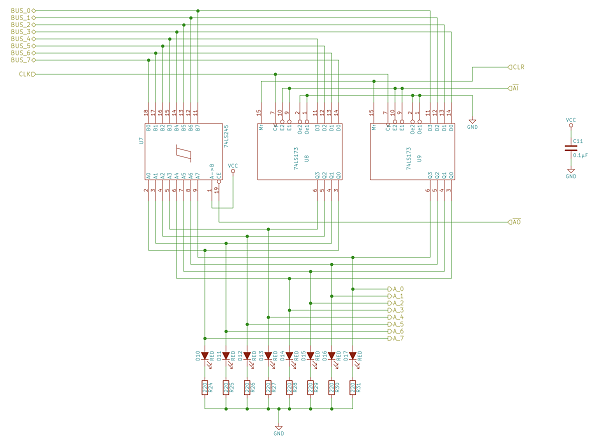
\includegraphics{8-bit-a-register}
  \caption{Schematic of the A register in Bean Eater's 8-bit computer \cite{eater2019highlevel}}
  \label{8-bit-a-register}
\end{figure}

\chapter{Hardware Specification \& Design}
This chapter of the report focuses on creating a comprehensive set of specifications for the computer
to be built as a part of the project and then provides a detailed listing of the design choices made to satisfy
the specifications provided. Since the design will be based on Bean Eater's 8-bit breadboard computer \cite{eater2019breadboard}, but it will also include parts of SAP-2 and SAP-3 \cite{malvino1992digital}. Most specification criterions will be phrased as additions and enhancements to the existing designs.

\section{Specification Guidelines}
The specifications which are about to be presented serve the purpose of adding functionality to the 8-bit breadboard computer such
that its educational potential is harnessed more effectively, while at the same time avoiding over-complication and over-extensions
of scope. As such, it makes sense to list some of the features which will \emph{fall out of the scope} of this build for practical
and time considerations.
\begin{itemize}
  \item Interrupts and Interrupt handling
  \item Processes (The computer will only run one process, there will be no threading interface/ no operating system)
  \item Floating-Point operations
  \item Support for any kind of advanced in-hardware operations (for example encryption)
  \item Native support for signed integers over 16 bits
  \item Graphical User Interfaces (GUIs)
  \item Input through traditional peripheral (mouse and keyboard)
\end{itemize}

\section{Major Architecture Changes}
The computer should broadly follow the architecture o the 8-bit computer designed by Malvino and Brown \cite{malvino1992digital} and built by Bean Eater \cite{eater2019breadboard}. The major architectural difference should be \emph{the extension to 16-bit words}.
Since the word length of the computer should be 16 bits, its bus and most of its modules should be extended to accommodate this extra capacity.

\subsection{Operational Enhancments}
Besides Addition and Subtraction, the computer should also implement \emph{bit-shifting} (both left and righ). Bit-shifting is a crucial operation which is very often performed to increase the efficiency of certain operations (for example, multiplication and division by 2 can be expressed in binary as a left or a right shift of 1 bit)

\subsection{I/O Enhancements}
Currently, the only way to provide input to the 8-bit computer is by \emph{manually} programming each memory address through dip-switches. This is slow, clunky and prone to errors. There should exist a mechanism to quickly program the computer, for example through an external \emph{microcontroller} like an Arduino. Besides this, there should also exist a way for the computer to request input \emph{while executing} from an external device like a microcontroller.
Similarly, to provide persistence to the values from calculated by the computer, instead of being able to display only one value at a time, the computer should also have the ability to communicate with an existing external device like a separate microcontroller, providing it with the values it has calculated. In turn, the microcontroller a the be connected to a regular personal computer and then programmed to display those values to the screen. Besides this, the computer should have a display capable of displaying
more than 4 characters and more than just numbers.

\subsection{Stack Operations}
The addition of a stack pointer would make subroutines, calls to subroutines and callbacks significantly easier. An effective
stack pointer just has to have the option to increment and decrement, in contrast to a simple program counter which just increments.
With this functionality, return addresses can be pushed on and popped off of the memory stack whenever they are required.

\subsection{Expanded Random Access Memory}
Eater's implementation has a very limited address space (4 bit address, which equates to 16 addresses). While from a theoretical
point of view, this is as close to a Turing Machine as a supercomputer with terrabytes of RAM (an ideal Turing Machine should have infinite memory), a more reasonable amount of memory (in the kilobytes range) would allow for far greater flexibility in software
applications. For this computer, a 16K memory (\(2^10 * 16\), or 10 bit address space) should be sufficent.

\subsection{Memory Layout}
Due to the added features, the memory layout of the 16-bit breadboard computer needs to be re-worked. As such, the following
layout is proposed:
\begin{itemize}
  \item From 0x000 to 0x1FF: Program Text
  \item From 0x200 to 0x3EF: Variables and Data
  \item From 0x3F0 to 0x3FF: Stack
\end{itemize}

\section{16-bit Breadboard Computer Layout}
Based on the previous specification, the computer to be built in this report should contain the following modules and
have the following physical layout:

\begin{figure}[h]
  \centering
  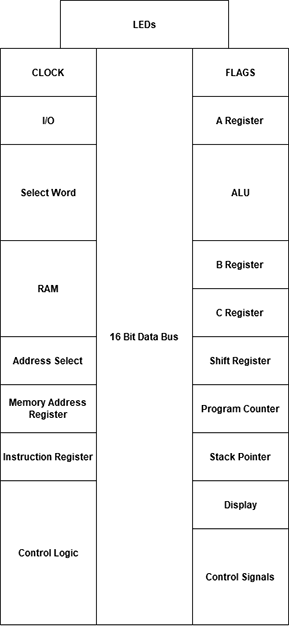
\includegraphics{16-bit-layout}
  \caption{High Level Module Overview and Layout of the 16-bit Breadboard Computer}
  \label{16-bit-layout}
\end{figure}
\clearpage

The updated computer specification contains the following modules, each of which will be followingly discussed in later sections:
\begin{enumerate}
  \item Common Data Bus \ref{common-data-bus}
  \item Data Bus LEDs \ref{data-bus-leds}
  \item Clock \ref{clock}
  \item A Register \ref{a-reg}
  \item B Register \ref{b-reg}
  \item Arithmetic-Logic Unit (ALU) \ref{alu}
  \item Flags Register \ref{flags}
  \item C Register \ref{c-reg}
  \item Shift Register \ref{shift-reg}
  \item Random Access Memory (RAM) \ref{ram}
  \item Program Counter \ref{pc}
  \item Stack Pointer \ref{stack-pointer}
  \item Display \ref{display}
  \item I/O \ref{io}
  \item Memory Address Register \ref{mar}
  \item Instruction Register \ref{ir}
  \item Word Selector \ref{word-select}
  \item Address Selector \ref{addr-select}
  \item Control Logic \ref{control-logic}
  \item Control Signals \ref{control-sigs}
  \label{module-list}
\end{enumerate}

\subsection{Common Data Bus} \label{common-data-bus}
The Common Data Bus acts as the communication medium of the computer. Drawing a parallel between \emph{computer design}
and \emph{human anatomy}, the data bus acts like the circulatory systems. It ensures all other components are connected
and can talk to each other. The Common Data Bus should be 16 bits wide, since the final system should have a word length of
16 bits. Since all other modules connect to the Data Bus, it makes sense to have it located centrally, between all other modules.
This way, no module has to have particularly long wires to interface with the Bus.

\subsection{Data Bus LEDs} \label{data-bus-leds}
This modules is as simple as it gets. It should be composed of just 16 LEDs, or Light Emitting Diodes, one on each Data Bus line,
so that whatever gets asserted at a certain point in time on the Bus can be visible. Besides this, it can also contain pull-down
resistors to ensure that, if no module asserts anything on the bus, it should default to low, or a logic 0.

\subsection{Clock} \label{clock}
The clock acts as the heart of the system. It provides a pulse under the form of a square wave, based on which all other components
do their job. The clock signal should be distributed to all other modules. Besides providing the square wave clock pulse an inverse,
or counter clock pulse should be available, as well as the ability to change the frequency and to completeley stop the square wave
and replace it with a manual button press for demonstrational and debugging purposes.
Finally, the clock should take in one signal as input, namely halt, or \emph{HLT},
which should completeley stop the clock regardless of operating mode. This will allow the computer to halt execution
if, for example, the program is finished. \\
\textbf{$Input Control Signals: HLT$} \\
\textbf{$Output Control Signals: CLK, \overline{CLK}$}

\subsection{A Register} \label{a-reg}
The A register is a 16-bit memory storage module. It should implement three functions. First, when its \emph{AI}
(A Register In) signal goes high, it should latch in the contents of the data bus on the rising edge of the next clock pulse.
The second function is to output its contents to the bus when its \emph{$\overline{AO}$} (A Register Out) signal goes low. Finally,
if the \emph{$\overline{RST}$} (Reset) signal goes low, it should clear out its contents and latch in a 0 on all bits. Additionally,
the A register should have a direct 16-bit connection to the \emph{Arithmetic Logic Unit}, or ALU \ref{alu}. \\
\textbf{$Input Control Signals: CLK, AI, \overline{AO}, \overline{RST}$}
\textbf{$Direct Connection to: ALU$}

\subsection{B Register} \label{b-reg}
Similarly to the A Register, the B Register should store 16 bits of data from the bus. It should have similar control signals,
\emph{BI, BO} and \emph{RST}, which perform equivalent functions. It should also have a direct 16-bit connection to the \emph{ALU}
\ref{alu}.
\textbf{$Input Control Signals: CLK, BI, \overline{BO}, \overline{RST}$}
\textbf{$Direct Connection to: ALU$}

\subsection{Arithmetic Logic Unit} \label{alu}
The Arithemtic Logic Unit, or ALU, is the module responsible with data procesing. It takes the contents from\emph{both A and B
registers} \ref{a-reg} \ref{b-reg} directly and adds them up. Is the \emph{SU} (Subtract) signal is provided, the contents of the
B Register \ref{b-reg} will be subtracted from the contents of the A register. If the \emph{$\overline{\varepsilon O}$} (Sum Out)
is taken low, the contents of the  ALU will be asserted on the data bus. The ALU also has a direct connection to the Flags Register
\ref{flags}. Over this connection, the ALU should provide three flags:
\begin{itemize}
  \item Parity Flag: whether the \emph{Least Significant Bit} is 0 or 1
  \item Zero Flag: wheter the content of the ALU is 0
  \item Carry Flag: wheter the result of the operation of the ALU is cannot be expressed within 16 bits
\end{itemize}
\textbf{$Input Control Signals: \varepsilon O, SU$}
\textbf{$Direct Connection to: A Register, B register, Flags Register$}

\subsection{Flags Register} \label{flags}
The Flags Register is essential towards ensuring the Turing completeness of the computer being built. Based on the state of the
flags, the computer can make branch decisions, which reflect the fact that Turing machines can make selective decisions based
on the symbol it has just read.
Essentially, the flags register serves the purpose to latch in the three flags provided by the ALU \ref{alu}: the Parity Flag, the
Zero Flag and the Carry Flag. When the \emph{FI} (Flags In) signal is taken high, on the next clock pulse it should latch in the
contents of those flags. Besides this, the Flags Register should clear its contetns when the \emph{$\overline{RST}$} (Reset) signal
is taken low. There is a direct connection between the Flags Register and the Control Logic module, as the flags play a role in
deciding what to do next. \\
\textbf{$Input Control Signals: CLK, FI$}
\textbf{$Direct Connection to: ALU$}

\subsection{C Register} \label{c-reg}
The C Register serves as a general purpose 16-bit register. It has signals similar to the other two registers, A \ref{a-reg} and
B \ref{b-reg}. When \emph{CI} (C Register In) goes high, on the next clock pulse the register should latch in the data word
asserted on the bus in its storage. IF \emph{$\overline{CO}$} (C Register Out) goes low, the register should assert its contents
on the data bus. IF \emph{$\overline{RST}$} (Reset) goes low, it should clear its contents and latch in onyl zeroes. There should
be no direct connection between the C register and any other registers. \\
\textbf{$Input Control Signals: CLK, CI, \overline{CO}, \overline{RST}$}

\subsection{Shift Register} \label{shift-reg}
The Shift Register is the other module of the 16-bit breadboard computer capable of conducting data processing tasks. First and
foremost, it should act as a normal register, so it should latch in the bus contents on the next clock pulse if the \emph{SI}
(Shift Register In) signal goes high, asserts its contents to the bus if \emph{$\overline{SO}$} goes low, and clears it contents
if \emph{$\overline{RST}$} goes low. Besides this, if \emph{SFL} (Shift Left) goes high, on the next clock pulse it should shift its
contents to the left by one bit and insert a 0 at the least significant bit of the data word. Similarly, if \emph{SFR}
(Shift Right) goes high, on the next clock pulse it should shift its contents one bit to the right and insert a 0 at the most
significand bit of the data word. \\
\textbf{$Input Control Signals: CLK, SI, \overline{SO}, SFL, SFR, \overline{RST}$}

\subsection{Random Access Memory (RAM)} \label{ram}
Random Access Memory, or RAM, is the equivalent of the tape on a Turing machine. It can be read from and written to, and it should
be large enough to accommodate algorithms, data and variables; all at the same time. Memory is organised in addresses. Each address
should store one 16-bit word of memory. A 10-bit address is deemed to be sufficent, so the computer should have a
\(2^10*16 = 16K\) memory space. The RAM module should also have a direct connection to the \emph{Address Selector}
\ref{addr-select} and to the the \emph{Word Selector} \ref{word-select}. The Address Selector serves a 10-bit address to the
memory, while the word selector serves a 16-bit data word to the RAM. If the \emph{RI} (RAM In) signal goes high, on the next clock
pulse the RAM Module should latch in the data word served by the word selector at the address provided by the address
selector. If the \emph{RO} signal goes low, the RAM module should assert the data word stored at the address provided by the
address selector on the data bus. Additionally, based on two control signals originating from toggle switches, \emph{PROG} and
\emph{ARDUINO}, the signal which governs the RAM writes can be changed. If \emph{PROG} is low, that means the computer is in run
mode, and the \emph{RI} signal controls writes. If \emph{PROG} is high, then the computer is in programming mode, and the
write signal is chosen based on the \emph{ARDUINO} signal. If \emph{ARDUINO} is low, then the writes are manually controlled
using a simple push button. If it is high, then an external \emph{Arduino Mega} \cite{arduino2020mega} controls the writes to
memory using a signal called \emph{$ARDUINO_WRITE$}. \\
\textbf{$Input Control Signals: CLK, RI, RO, PROG, ARDUINO, ARDUINO_WRITE$} \\
\textbf{$Direct Connection to: Word Selector, Address Selector, Arduino Mega$}

\subsection{Program Counter} \label{pc}
The Program Counter serves the purpose of keeping track of the current address which should be executed. As such, it should
be a 10-bit register, to ensure coverage of the entire address space of the computer. If the \emph{CE} (Counter Enable) signal
goes high, on the next clock cycle the program counter should count up one in binary from the value it has currently latched
in its storage and then latch this new value in. If the \emph{$\overline{JMP}$} (Jump) signal goes low, on the next clock pulse the
program counter should latch in whatever value is asserted on the 10 loweest bits of the bus in its register. If
\emph{$\overline{CNT_O}$} (Counter Out) goes low, the value latched in the program counte should be asserted on the data bus.
If \emph{$\overline{RST}$} (Reset) goes low, the program counter should clear out its contents and latch in zeroes on all bits. \\
\textbf{$Input Control Signals: CLK, CE, \overline{JMP}, \overline{CNT_O}, \overline{RST}$}

\subsection{Stack Pointer} \label{stack-pointer}
Tha stack pointer should essentially be a register holding a 10-bit address, but accepting only a small subsection of the address
space (from 0x3F0 to 0x3F). This means that the stack should be 16 addresses tall. If the \emph{$\overline{ST_I}$} (Stack Increment)
signal goes low, on the next clock pulse, the stack pointer should increment by one. If \emph{$\overline{ST_D}$} (Stack Decrement)
goes low, the stack pointer should decrement by one on the next clock pulse.
On \emph{$\overline{ST_J}$} (Stack Jump) going low, on the next clock pulse the stack pointer should latch in the address asserted
on the bus in its register, assuming it is a valid stack address. If \emph{$\overline{ST_O}$} goes low, the stack pointer should
assert the address it has stored out on the bus. Finally, if \emph{$\overline{RST}$} (Reset) goes low, the stak pointer should reset
to zero. \\
\textbf{$Input Control Signals: CLK, \overline{ST_I}, \overline{ST_D}, \overline{ST_J}, \overline{ST_O}, \overline{RST}$}

\subsection{Display} \label{display}
The Display module is the main way through which the computer can interface with the user. It should have the ability to display
both alfanumeric characters and digits and it should feature at least 2 lines of 16 characters each. When the \emph{OUT} (Output)
signal goes high, the display should take a word of data from the bus and interpret it as the next character to be written to the
screen. \\
\textbf{$Input Control Signals: OUT$}

\subsection{I/O} \label{io}
Besides a display, the computer should also feature a bidirectional interface to another mirocontroller. In this case,
the interface should be to an \emph{Arduino Mega} \cite{arduino2020mega}. If the \emph{$\overline{E}$} (Enable) signal goes low,
based on the \emph{$R/\overline{W}$} (Read/Write) signal, the computer should interact with the Arduino. If the
\emph{$R/\overline{W}$} signal is high the computer should read a word of data from the arduino, so that word of data should be
asserted on the bus. If the \emph{$R/\overline{W}$} signal is low, the Arduino should read a word of data from the bus (and
consequently displayed to the user). \\
\textbf{$Input Control Signals: \overline{E}, R/\overline{W}$} \\
\textbf{$Direct Connection to: Arduino Mega$}

\subsection{Memory Address Register} \label{mar}
The memory address register, or MAR, is a 10 bit register. It connects directly to the address selector \ref{address-select} and
there is no other way to get the information latched into it. If the \emph{MI} signal goes high, on the next clock pulse the MAR
will latch into its storage the 10 least significant bits asserted on the bus. if \emph{$\overline{RST}$} goes low, the MAR will
clear its contents and write zeroas to all 10 bits. \\
\textbf{$Input Control Signals: CLK, MI, \overline{RST}$} \\
\textbf{$Direct Connection to: Address Selector$}


\subsection{Instruction Register} \label{ir}
The Instruction Register, or IR, is a 16-bit register which holds the next instruction to be processed. It is special in that
its most significant 6 bits have a different meaning. They represent the opcode for the current instruction and are directly
connected to the Control Logic module \ref{control-logic}. When the \emph{II} (Instruction Register In) signal goes high, on the
next clock pulse the instruction register should latch in the data word asserted on the bus in its storage. If the
\emph{$\overline{IO}$} (Instruction Register Out) signal goes low, the register should assert its least significand 10 bits to the
bus. If \emph{$\overline{RST}$} (Reset) goes low, the instruction register should reset and latch in zeroes on all 16 bits. \\
\textbf{$Input Control Signals: CLK, II, \overline{IO}$} \\
\textbf{$Direct Connection to: Control Logic$}


\subsection{Word Selector} \label{word-select}
The Word Selector is a special module, in that it serves the purpose of selecting between different sources of data and feeding
them into the RAM module \ref{ram}. There are three possible sources of data
\begin{enumerate}
  \item The Data Bus
  \item Dip Switches
  \item An Arduino Mega
\end{enumerate}
The Data Bus is the first and most straight forward data source. A 16-bit data word can be taken from the bus and then passed on
to memory. The second source are Dip Switches. Dip Switches are rows of small binary switches, which can be used to manually feed
binary data into a digital system. The last possible source of data is an arduino mega. The choice of data to be fed forward is
governed by two control signals, \emph{PROG} and \emph{ARDUINO}. If \emph{PROG} is low, data from the data bus will be selected,
regardless of the state of \emph{ARDUINO}. If \emph{PROG} is high, that means that the computer is in programming mode. In this
mode, the data source depends on the \emph{ARDUINO} control signal. If this signal is high, then data will be fed forward from
an external Arduino Mega \cite{arduino2020mega}. If it is low, then a series of 16 dip switches will be used to manually program
the computer.  \\
\textbf{$Input Control Signals: PROG, ARDUINO$} \\
\textbf{$Direct Connection to: RAM, Arduino Mega$}

\subsection{Address Selector} \label{address-select}
Similar to the Word Selector \ref{word-select}, the Address Selector selects between different address sources to provide a 10-bit
address to  the RAM module \ref{ram}. There are three possible data sources:
\begin{enumerate}
  \item The Memory Address Register \ref{mar}
  \item Dip Switches
  \item An Arduino Mega
\end{enumerate}
The choice of data source is defined by two control signals, \emph{PROG} and \emph{ARDUINO}. If \emph{PROG} is low, then the
computer is in run mode and the address latched in the \emph{MAR} \ref{mar} is fed forward to RAM. If it is high, then that means
the computer is in programming mode and the address choice is governed by the \emph{ARDUINO} control signal. If it is low, then
the memory address will be manually chosen using a series of 10 Dip Switches. If it is high, then an external
Arduino Mega \ref{arduino2020mega} will be the address source. \\
\textbf{$Input Control Signals: PROG, ARDUINO$}
\textbf{$Direct Connection to: RAM, Arduino Mega$}

\subsection{Control Logic} \label{control-logic}
To draw another parallel to human anatomy, the control logic module can be thought of as the ~~brain`` of the computer.
It takes in the 6-bit opcode from the Instruction Register \ref{ir}, the 3 flags from the Flags Register \ref{flags}, as well as
a 3 bit number representing the ~~step`` of the current instruction which is to be executed and decides based on these pieces
of information which control signals to keep active on the next clock cycle. It also maintains an internal 3 bit counter which
counts on the inverted clock or counter clock signal to provide the 3-bit step. \\
\textbf{$Input Control Signals: \overline{CLK}$}
\textbf{$Output Control Signals: HLT, \overline{RST}, AI, \overline{AO}, BI, \overline{BO}, \overline{\varepsilon O}, SU, FI, CI, \overline{CO}, SI, \overline{SO}, SFL, SFR, RI, RO, CE, \overline{JMP}, \overline{CNT_O}, \overline{ST_I}, \overline{ST_D}, \overline{ST_J}, \overline{ST_O}, OUT, \overline{E}, R/\overline{W}, MI, II, \overline{IO}$}
\textbf{$Direct connection to: Instruction Register, Flags Register$}


\subsection{Control Signals} \label{control-sigs}
The Control Signals Module is used to visualise which control signals are active at any given time. This module should
essentially consist of a labeled LED on each control signal.

\section{Specification Conclusion}
This concludes the specification phase of the project. The next step is to design each module to this specification.

\section{Design}
This section of the report focuses on the design process for the individual modules of the 16-bit breadboard computer.
The goal is to satisfy all specification criterions designated in the last section, while also adhering to the general goal
and philosophy of the project as close as project. First of all, the design process will be documented and analysed. After that,
the tools used to facilitate the design will be presented. Finally, each module design will be presented and scrutinized.

\subsection{How to design a 16-bit computer module}
In order to successfully come up with a design for a computer module while also meeting the specification outline and
keeping the schematics as simple as possible, a simple yet effective design process has been implemented. It consists
broadly of 4 distinct steps:
\begin{itemize}
  \item Chip Discovery
  \item Chip Analysis
  \item Chip Selection
  \item Schematic Creation
\end{itemize}

\subsection{Chip Discovery and Analysis}
The first step towards the design of a 16-bit computer module is the \emph{integrated circuit/IC/chip} discovery and analysis phase.

\paragraph{Why use Integrated Circuits/Chips?}
Since the general goal of the project is to produce a Turing complete computer which is as simple as possible to understand
and also relies as little as possible on any other form of abstraction, one might argue that using integrated circuits, or chips,
woud be against that goal. While this argument is theoretically correct, it doesn't take into account any practical considerations.
The lowest level of the technology stack from which one could go ahead and phisically construct a computer would probably be
the transistor. That being said, trying to implement any computer, let alone a 16-bit computer with many different modules, would
be next to impossible to successfully do within the time frame of this project and also without a team of people. The physical
scale would be many, many times what the scale of the computer built in this project is and the amount of errors which would arise
from connecting individual transistors together by hand would probably be so large, that one would quickly lose interest in
finishing the build. As such, simple integrated circuits pose themselves as a great compromise. These circuits, which usually
implement simple logic functions, like \emph{AND, OR, Inverter, etc.}, or even a little bit more complex functions,
like \emph{registers or binary adders}, can each contain tens to hundreds of individual transistors. That being said, they should
all be simple enough so thatthe functionality provided by each chip should be \emph{understandable down to the transistor level}.

\paragraph{Understanding Integrated Circuits}
While this may sound daunting at first, it can actually be relatively straight forward. Individual logic gates are each made up of
a few transistors. For example, Ben Eater has created an excellent YouTube tutorial on how to create logic gates out of transistors
\cite{eater2015logicgates}. Armed with this knowledge, we can now approach the datasheet of a particular circuit we intend to use.
For example, on page 2 of the datasheet of the \emph{74LS157} \cite{74ls157} multiplexer chip, we can find the logic diagram.
By analysing the logic diagram and calculating boolean outputs based on arbitrary inputs and then comparing the results
to the truth table of the chip provided on the first page of the datasheet, one can verify that the chip actually implements its
specified interface in a logical manner. This can be applied to all chips which are considered to be potential building blocks
for a module, as long as the individual chip complexity is relatively limited.

\subsection{Where to look for Integrated Circuits}
There are three main sources of chips which where consulted when conducting chip discovery. The first one was the Wikipedia list
of chips from \emph{7400} family \cite{wikipedia74lslist}. This particualr logic family was chosen because it is the most popular
and widley spread and adopted logic family in the world \cite{wikipedia74ls}. The second souce of chips, which served as a quick
reference, was Eater's part listing for his 8-bit breadboard computer build \cite{eater2020parts}. Since the 16-bit computer which
is to be built is largley based around the 8-bit computer built be Eater, many of the chips used in the 8-bit version will also
work in modules of the 16-bit version. Finally, for the few chips which were needed but weren't part of the 7400 family,
the websites of the retailers from which the chips were to be bought were searched. Two retailers were used, \emph{Mouser UK}
\cite{mouser} and \emph{Farnell UK} \cite{farnell}.

\subsection{Chip Selection}
Usually, the particular functionality of the module which is to be designed drastically boils down the list of potential chips.
For example, when designing a simple 16-bit register, like the \emph{A register} \ref{a-reg}, the \emph{74LS273} 8-bit flip-flop
\cite{74ls273} poses a great option. By just putting two \emph{74ls273} chips next to each other, most of the functionality of the
register has been designed. Whenever there is a need for extra functionality, for example in the case of the \emph{74ls273}
where there is no enable line, additional logic can be implemented using chips containing simple logic gates, like \emph{AND, OR,
NOT}. In this case, the clock signal can be AND'ed together with the \emph{AI} line to ensure that the register only reads from the
data bus when the control signal is set high.

\subsection{Schematic Creation}
With the right chips chosen for a module, the next step is to create a module schematic, which serves as a blueprint or design
document. The open-source computer-aided design software chosen to facilitate the creation of module schematics is \emph{KiCad}
\cite{kicad}. An overview of the application, as well as of the process of designing 16-bit computer modules with it will be
presented in detail in the next section.

\subsection{Electronic Design Tools with KiCad/Eeschema}
The main tool used to to design schematics for the 16-bit breadboard computer is \emph{KiCad} \cite{kicad}. KiCad is a broad and
mature electronics design software widley used in industry. It contains many tools which together from a tightly integrated
toolchain for designing complex electronics from the concept phase all the way to the printed circuit board. Since the goal of the
project is to build a computer on breadboards by hand and not create printed circuit boards, only the first step of the KiCad
pipeline has been used, namley \emph{Eeschema} \cite{eeschema}.

\paragraph{Eeschema}
\emph{Eeschema} is a electronic schematic computer design software. It is fully featured, easily accessible and has a relatively
shallow learning curve. By using \emph{Eeschema,} the entire module design process has been streamlined significantly.

\begin{figure}[h]
  \centering
  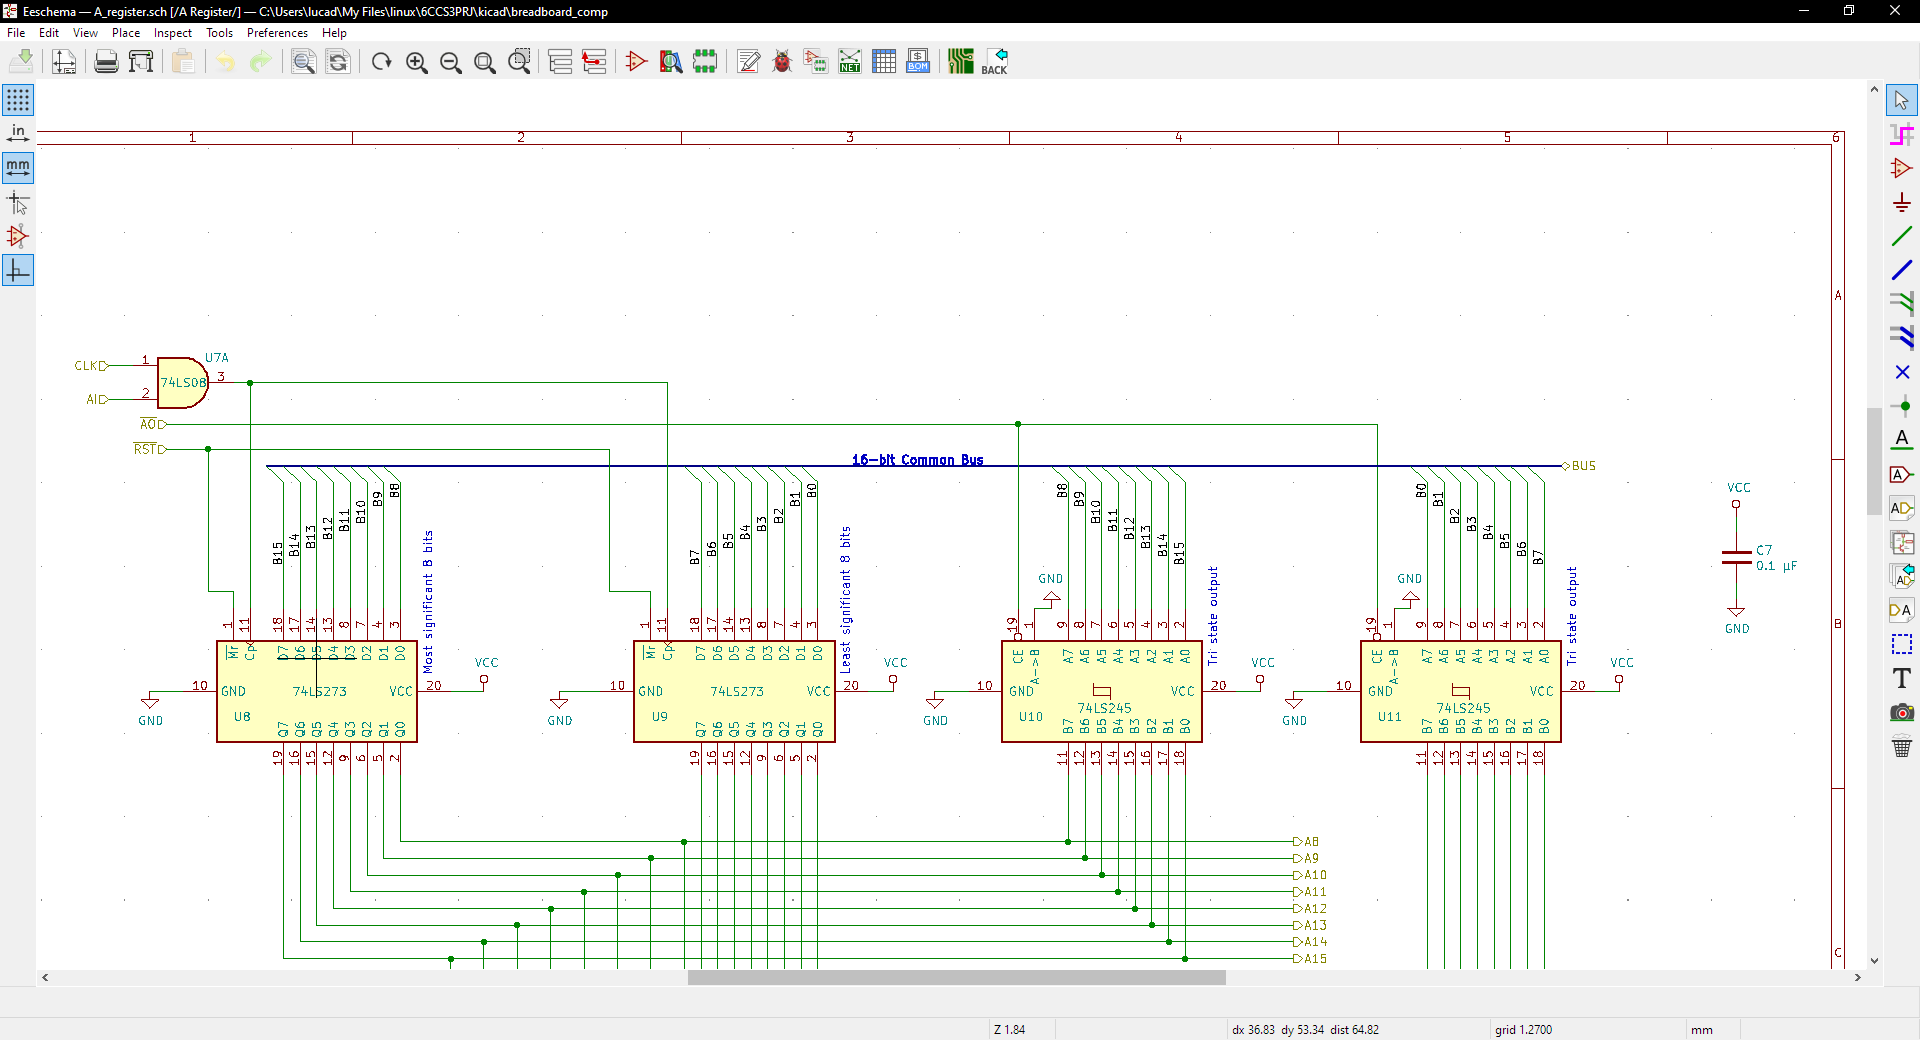
\includegraphics[scale=0.3]{eeschema}
  \caption{Eeschema Schematic Design software - part of the KiCad suite}
  \label{eeschema-interface}
\end{figure}
\clearpage

In the following paragraphs the most important features of Eeschema will be presented.

\paragraph{Intuitive Interface}
The graphical user interface provided by Eeschema is similar to many other widley used photo or video editing software packages.
As such, navigation is easy and intuitive. All tools and commands can be accessed both by pointer and keyboard, so one can become
proficient in whatever interface method is preferred. Drag and drop functionality allows the user to easily reposition misplaced
or misalligned circuits and components.

\paragraph{Hierarchical Sheets}
Hierarchical sheets is an Eeschema feature which allows one to embed entire schematics inside other schematics and seamlessly
transition between child and parent schematics. This is a great way to organise the modular design of the 16-bit breadboard
computer. Besides this, Eeschema offers the option to import input and output pins from the child schematic into the parent,
so that they can be connected to the wider circuit. This makes designing a high-level overview diagram significantly easier.

\paragraph{Bus connections}
Wiring up 16 separate wires which are connected to most modules as both input and output can be extremley tedious. Fortunatley,
\emph{Eeschema} offers the option to ~~bundle up'' mutliple wires as a single Bus and then have connections going in and out
of that single wire. Besides this, \emph{Eeschema} can resolve which pins are connected to which over the bus by use of labels
on the inputs and outputs \ref{ee-bus}.

\begin{figure}[h]
  \centering
  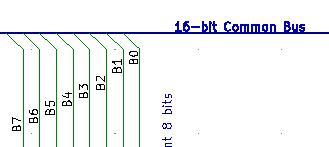
\includegraphics{ee-bus}
  \caption{Labeled Bus Connections in Eeschema}
  \label{ee-bus}
\end{figure}

\paragraph{Integrated Circuit Database}
\emph{Eeschema} ships with a pre-loaded database of commonly used chips and circuits, called the \emph{Symbol Library}.
This makes rapid schematic prototyping possible by just looking up potential circuits for the module and then dragging and dropping
them into the worksheet and then seeing if the connections would match up.

\begin{figure}[h]
  \centering
  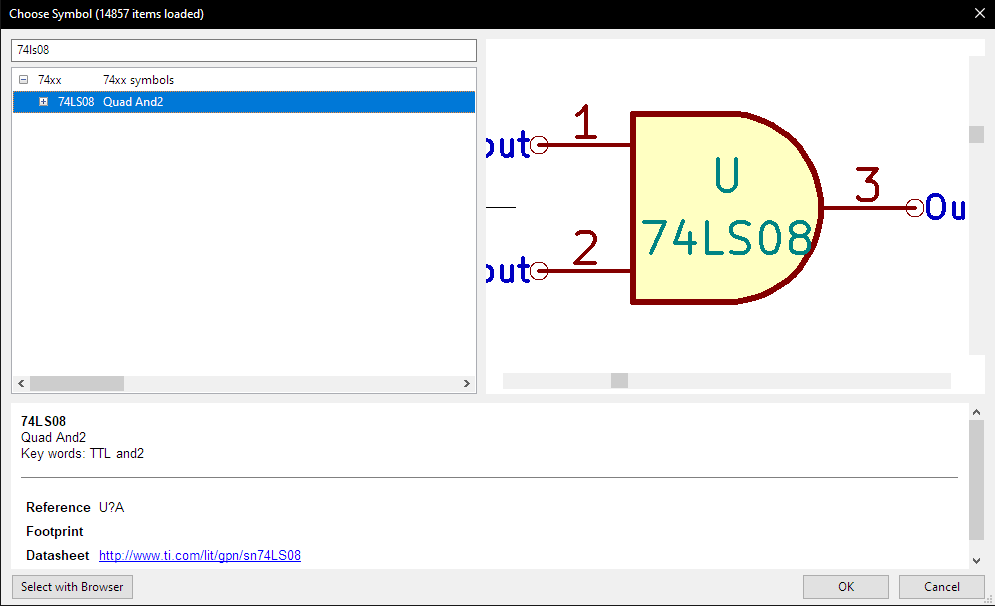
\includegraphics[scale=0.5]{ee-circuit-db}
  \caption{Component Database in Eeschema}
  \label{ee-circuit-db}
\end{figure}

\paragraph{Symbol Editor}
In the rare case where the \emph{Symbol Library} didn't contain a circuit needed for a module, \emph{Eeschema} provides
a simple circuit symbol editor. This ensures that the final schematics produced were accurate and reliable, regardless of wherer
the chip symbols were origianlly available in \emph{Eeschema} or not.

\begin{figure}[h]
  \centering
  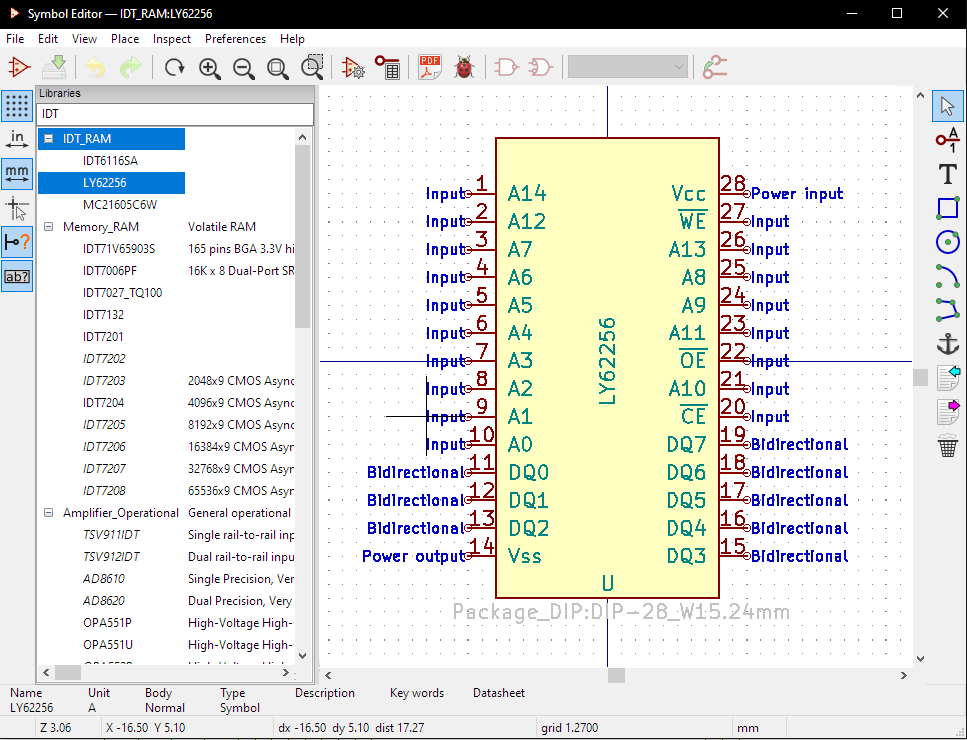
\includegraphics[scale=0.4]{ee-editor}
  \caption{Symbol editor in Eeschema}
  \label{ee-editor}
\end{figure}

\paragraph{Electrical Rules Check}
Besides providing an easy to use interface for designing accurate schematics, \emph{Eeschema} also offers active help in the
design process. By using the electrical rules checker, \emph{Eeschema} can check all connections against a user-defined set of
rules and report errors. This can be used to detect potetential human errors or even chip incompatibilities and resolve them
early on.

\begin{figure}[h]
  \centering
  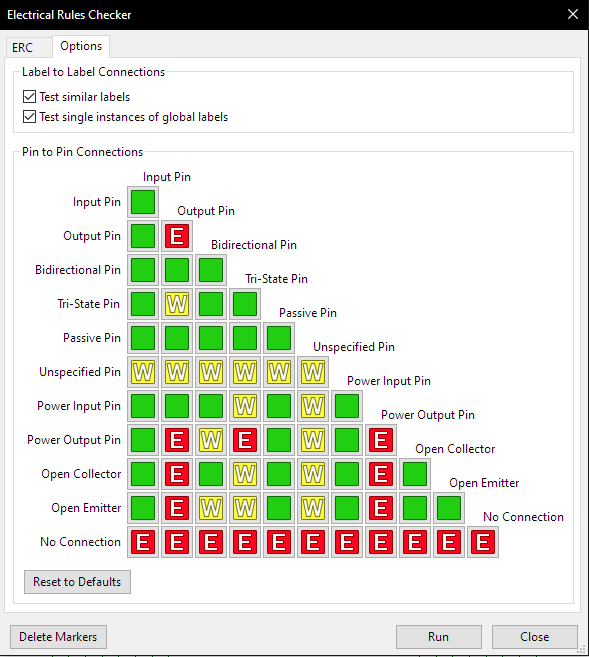
\includegraphics[scale=0.5]{ee-rules}
  \caption{The Eeschema Electrical Rules Checker}
  \label{ee-rules}
\end{figure}

\paragraph{Automatic Annotation}
When designing electrical circuits, it is common to use many identical or similar circuits next to one another. As such,
when actually building the circuit, one can be confused about which chip correlates to which symbol in the schematics.
To solve this, \emph{Eeschema} assignes a unique identifier, or annotation, to each symbol. This annotation process can be
done automatically.

\paragraph{Bill of Materials}
\emph{Eeschema} can also generate a bill of materials, or \emph{BOM}, based on all the symbols present in the schematic and
hierarchical schemaitcs. The BOM is essential towards ensuring that all needed components are purchased.

\begin{figure}[h]
  \centering
  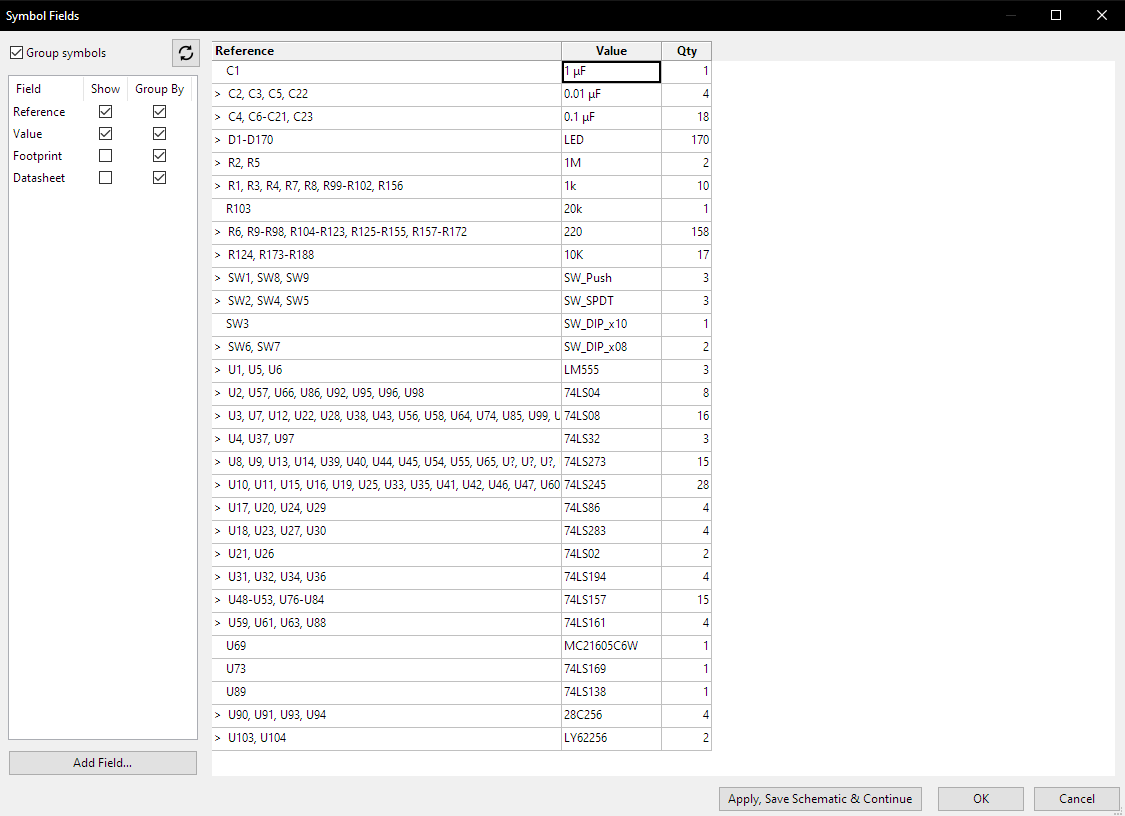
\includegraphics[scale=0.4]{ee-bom}
  \caption{Simple Bill of Materials generated by Eeschema}
  \label{ee-bom}
\end{figure}

\paragraph{PDF export}
Finally, Eeschema has been outfitted with an ~~Export to PDF'' option. This makes printing and compiling of the
schematics into other documents, like this report, significantly easier.

\subsection{Eeschema Design Process}
The following design process has been followed when creating schematics for a module as a part of the 16-bit breadboard
computer:
\begin{enumerate}
  \item Make an adequate chip selection
  \item Create a new hierarchial sheet and enter it
  \item Use the Symbol Editor to create chip symbols (in case the chips don't exist in the Symbol Library)
  \item Place all needed chips in the schematic
  \item Place all external control and I/O pins
  \item Connect all the pins apropiateley
  \item Leave the hierarchical sheet and import all I/O and control pins
  \item Run the automated annotation tool
  \item Run the electrical rules checker
  \item Correct any errors
\end{enumerate}

\subsection{Finalised 16-bit breadboard computer design and schematics}
The tools and processes discussed in the previous sections where extensivley used to produce the final schematics
for the 16-bit breadboard computer, which were used as templates for the physical implementation of the computer.
This section presents and discusses the schematics and the design decisions which were made during their creation.

\paragraph{High-Level Schematic}
The high-level schematic provides a layout and scale overview for the finished computer. It also contains the \emph{Data Bus LEDs}
module \ref{data-bus-leds}, as well as the actual \emph{Common Data Bus} \ref{common-data-bus}, to which all components connect.
Towards the bottom of the schematic the \emph{LEDs} module \ref{control-sigs} can also be found.

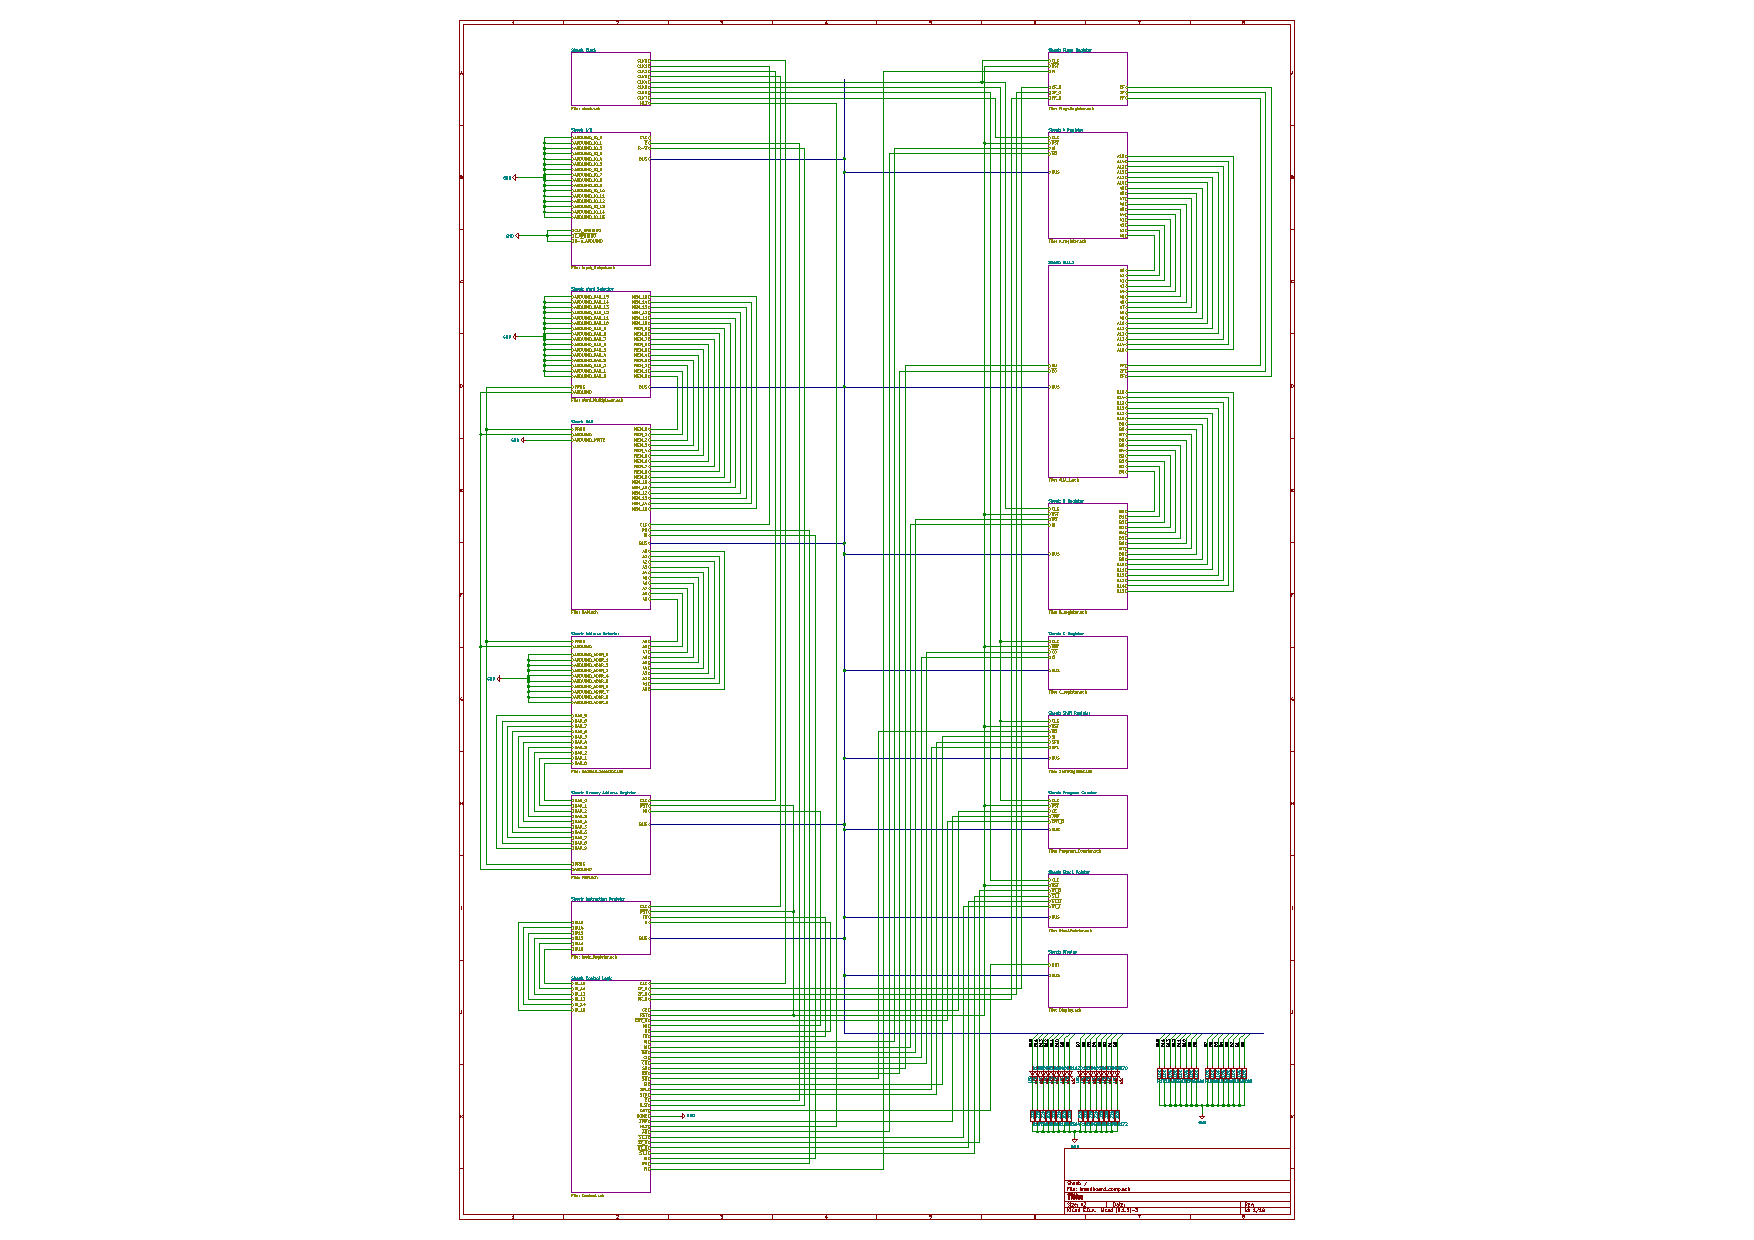
\includepdf[page={1}]{./pdf/kicad}
\clearpage

\paragraph{Clock} \ref{clock}
The clock module is very similar to the clock designed and built by Ben Eater \cite{eater2020clock}. It uses \emph{555 timers}
\cite{555} to generate a square wave which acts as the clock for the system. The \emph{555} is presented in all three most commonly
used configurations:
\begin{itemize}
  \item \emph{Astable: } it oscillates between to states (This 555 generates the main clock)
  \item \emph{Monostable: } it always ~~settles down`` to one state after a short period of time (used for the manual push-button
  clock mode)
  \item \emph{Bistable: } it has two states between which it can toggle (used for the toggle switch which goes from automatic to
  manual mode)
\end{itemize}
The clock-pulse generating \emph{555} is connected to a variable resistor which can be adjusted to increase or decrease the
frequency accordingly. A simple combinatorial circuit is used to select the appropiate clock signal and inhibit it if the \emph{HLT}
 (Halt) signal is active. The main addition to the Eater design is a \emph{74ls245 buffer} \cite{74ls245} used to amplify and
 isolate clock signals going to each module.

 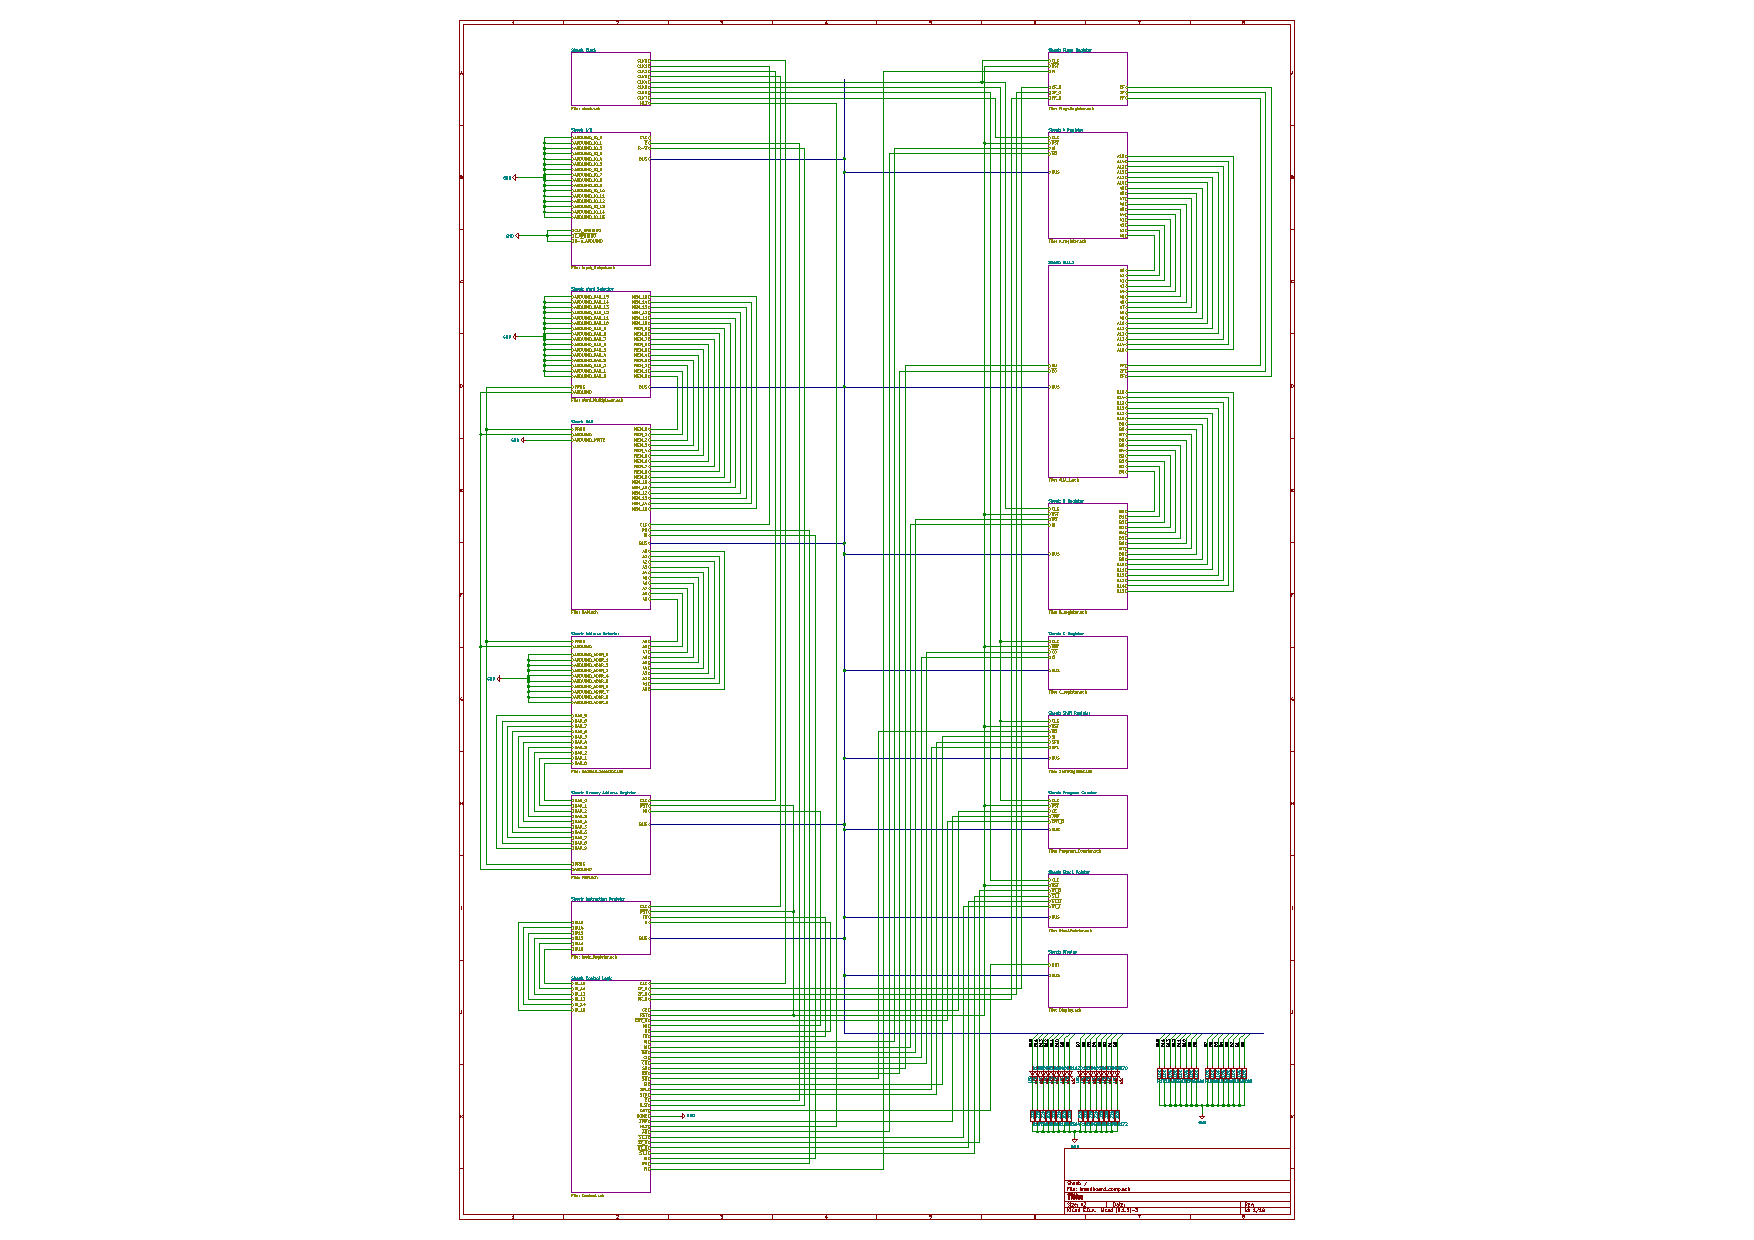
\includepdf[page={2}]{./pdf/kicad}

\paragraph{A Register} \ref{a-reg}
The A register consists of two \emph{74ls273} \cite{74ls273} 8-bit flip-flop chips and two \emph{74ls245} \cite{74ls245} buffer
interfaces to the bus. The buffers are \emph{tri-state} buffers, which means that they can pass through their input, either high or
low, or they can  disconnect their input from their output by putting themselves in a high-impedence state. This functionaility,
used across most modules which interface with the bus, is used to allow the register to assert its contents onto the bus when
reading from it (this happens when the \emph{$\overline{AO}$} signal is taken low). Writing to the register is handled by
ANDing together the \emph{AI} signal with the clock pulse. The contents of the A, which can be foud on the \emph{Q} pins, are
connected directly to the \emph{ALU} \ref{alu}.

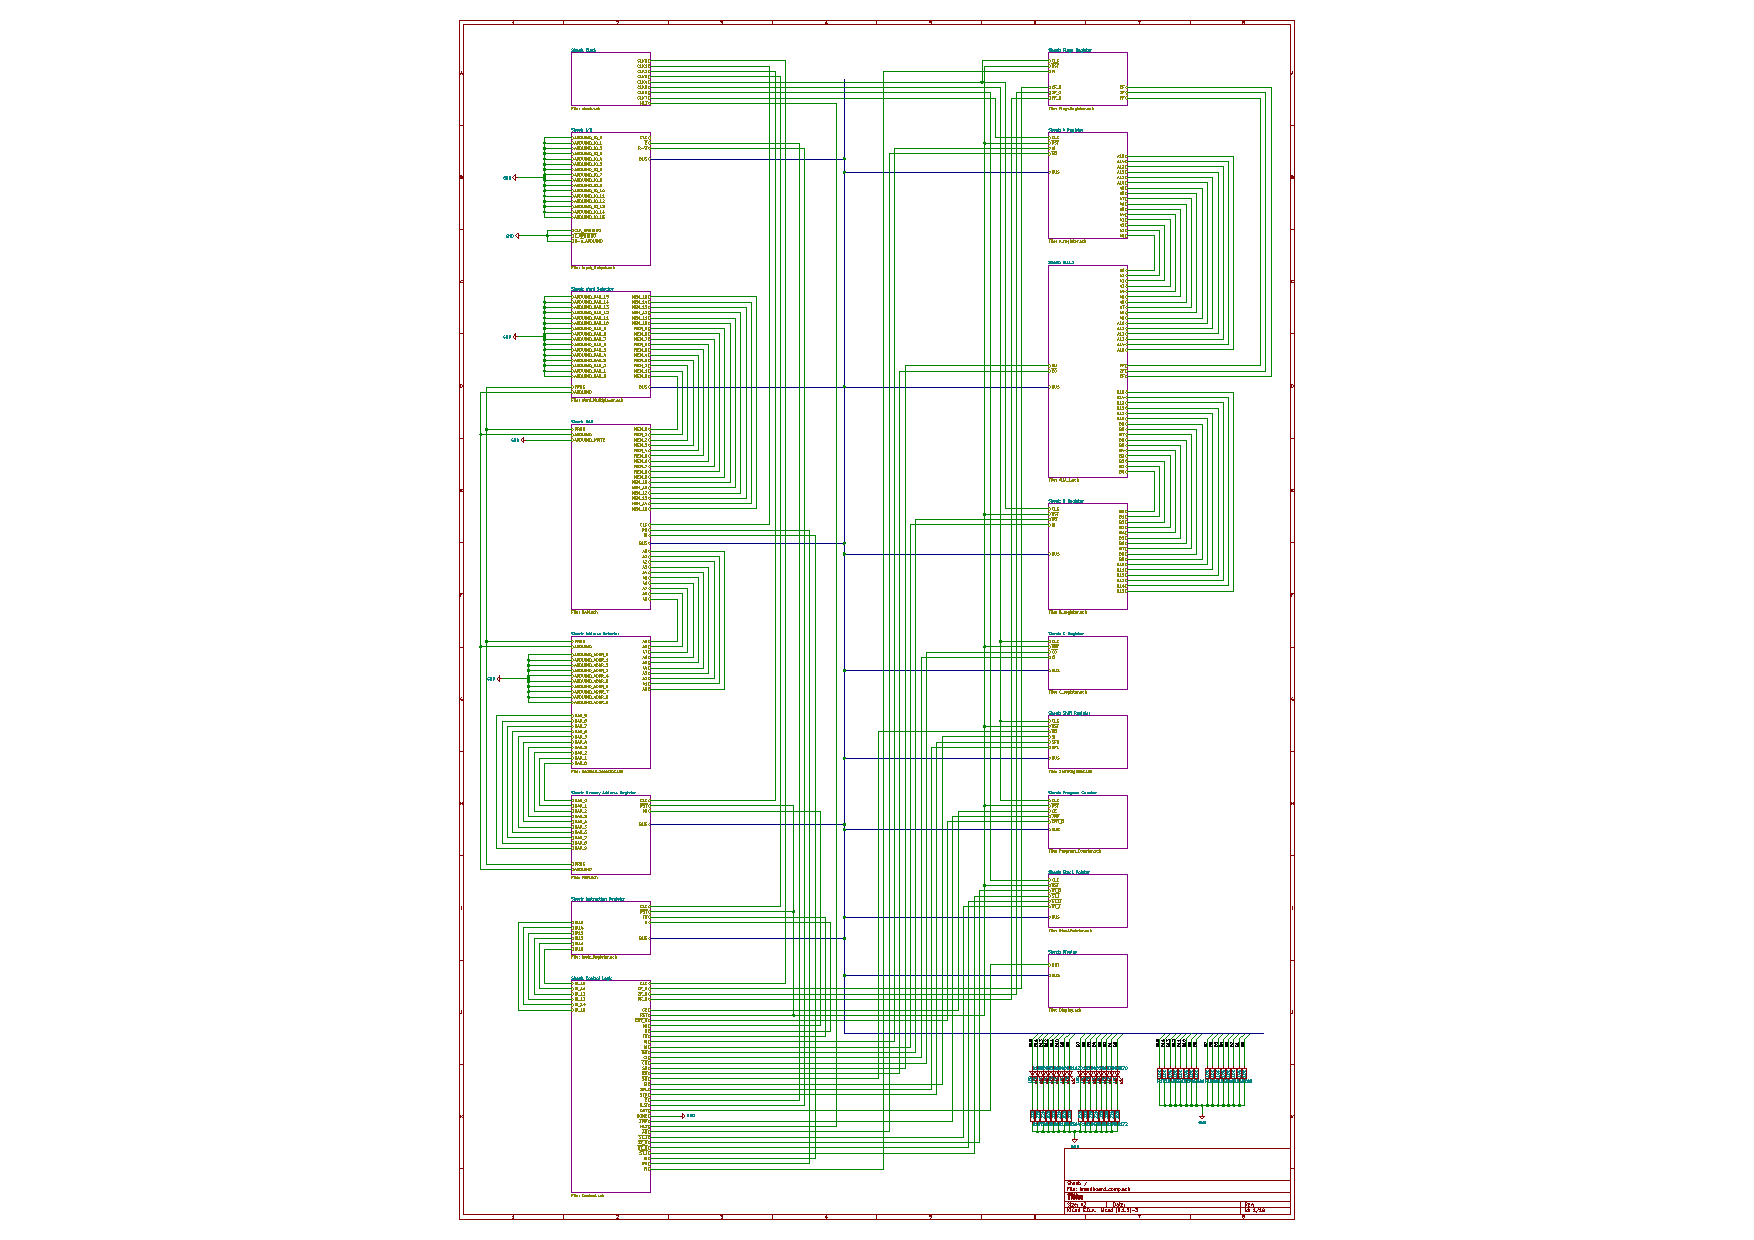
\includepdf[page={3}]{./pdf/kicad}

\paragraph{B Register} \ref{b-reg}
The B register is built essentially the same as the A register.

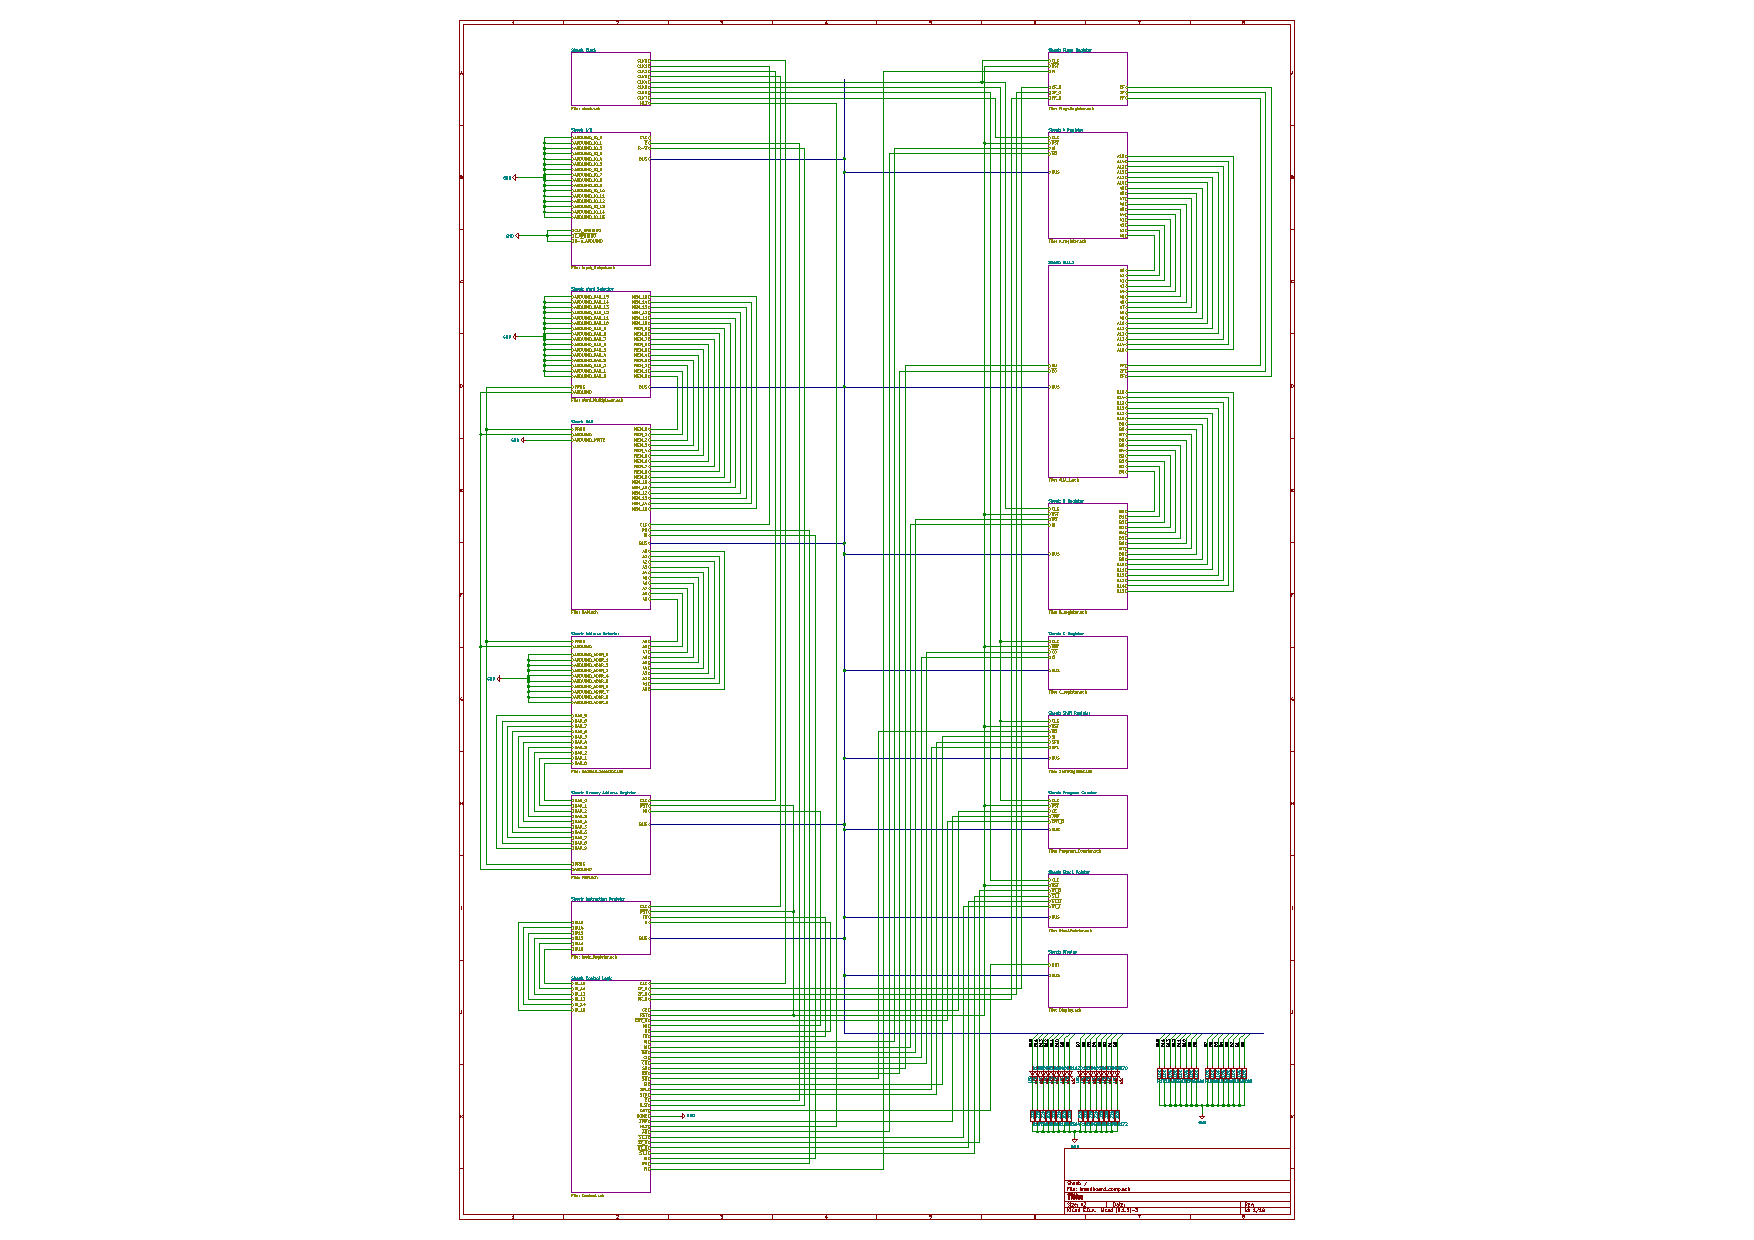
\includepdf[page={4}]{./pdf/kicad}

\paragraph{Arithmetic-Logic Unit} \ref{alu}
The \emph{ALU} has been designed around the \emph{74LS283} \cite{74ls283} chip. It contains a 4-bit binary full adder.
They can be chained together by connecting the Carry-Out of one chip to the Carry-In of the next chip. This way, by using 4
chips, a full 16-bit adder can be constructed. The A inputs are connected to the A register \ref{a-reg} and the B inputs
are conected to the B register \ref{b-reg}. The sum output is connect to two \emph{74LS245} \cite{74ls245} buffers which make the
connection to the data bus. To achieve subtraction functionality, the inputs from the B register are converted to two's complement
binary  notation, since subtracting a value equates to adding up the same negative value. To convert a positive binary value to a
two's complement negative value of the same magnitude, all 16 bits have to be flipped and then 1 has to be added to the number.
Flipping the bits is accomplished using the \emph{74LS86} \cite{74ls86} , which provides four independet XOR (exclusive or) gates.
By XORing each bit of the bit register with the value of the \emph{SU} control signal, each bit will just pass through the gate
if \emph{SU} is low and it will be flipped if \emph{SU} is high. Besides this, \emph{SU} is also connected directly to the Carry-
In Input of the first \emph{74LS283} full adder chip, to artificially add one to the final sum, representing the one which needs
to be added in for the two's complement form of the B register contents. \\
The \emph{ALU} also has three \emph{flag signals} which go out to the \emph{Flags Register} \ref{flags}. These are the \emph{Parity
Flag (PF)}, which represents the state of the lowest-significand bit of the sum, the \emph{Zero Flag (ZF)}, which is high if the
sum is 0 and low otherwise, and the \emph{Carry FLag (CF)}, which is set if the sum inside the \emph{ALU} cannot be expressed
within 16 bits. These flags can be used to make branching decisions based on the result of a calculation. The \emph{Carry Flag} and
\emph{Paritiy Flag} are straight-forward to obtain. The \emph{Carry Flag} is the Carry-Out pin of the most-significand adder
circuit. The \emph{Parity Flag} is the least significand sum pin of the least significand adder circuit. To calculate the
\emph{Zero Flag}, \emph{NOR} (inverted or) gates are employed on each pair of two sum bits. These gate can be found on the
\emph{74LS02} \cite{74ls02} chips. If any of the sum bits goes high, then the output of at least one \emph{NOR} gate will go low.
Subsequently, all \emph{NOR} outputs are ANDed together using successive \emph{AND} gates found on \emph{74LS08} \cite{74ls08}
chips. By using the and operator, if any one of the \emph{NOR} gates goes low, then the final output, which is the \emph{Zero Flag},
will go low. The only case where the \emph{Zero Flag} will go high is if all sum bits are 0.

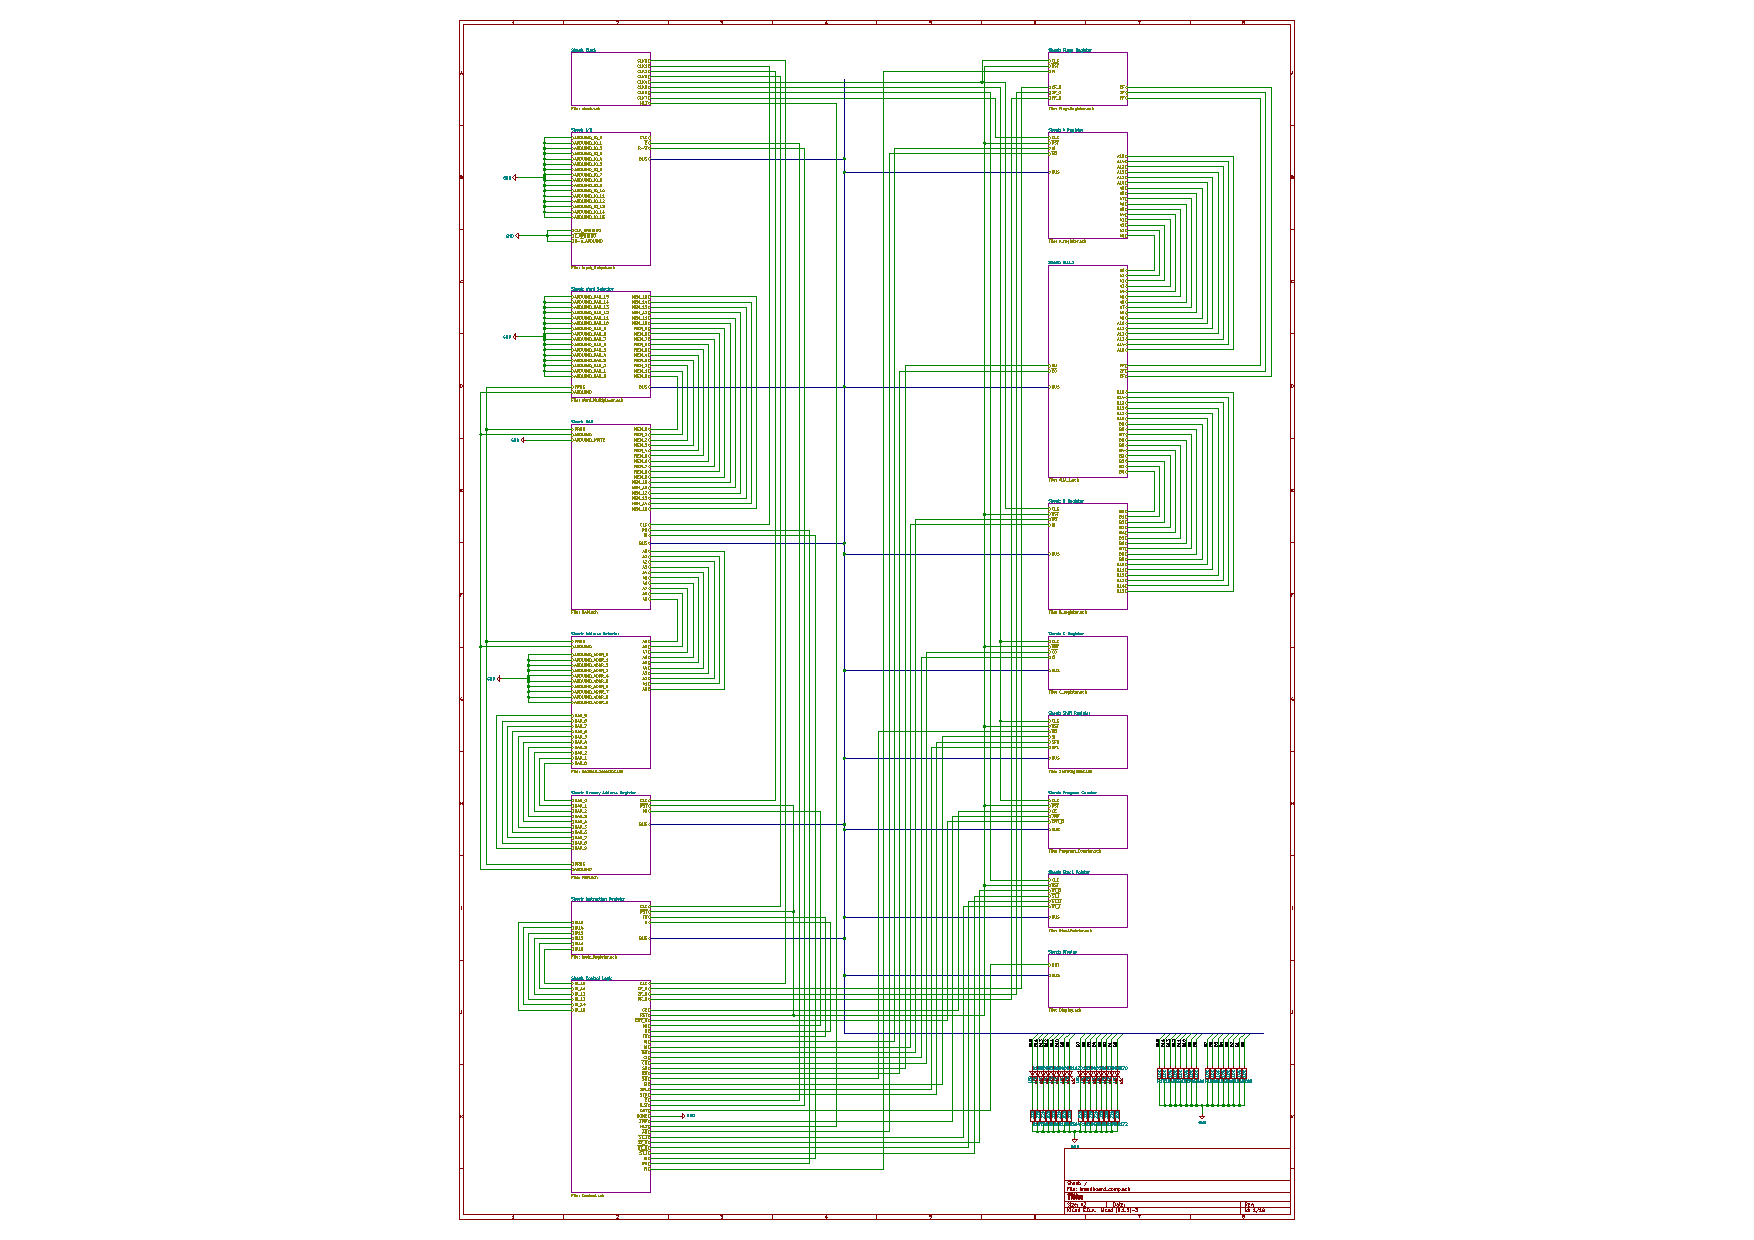
\includepdf[page={5}]{./pdf/kicad}

\paragraph{Flags Register} \ref{flags}
The Flags register consists of just one \emph{74LS273} \cite{74ls273} and some simple logic to handle the selective reads.
Allthough it is inneficient to use an 8-bit register to store only three bits, this design decision has been made because
the \emph{74ls273} is used in many other modeuls of the system and to avoid having to understand how another chip works and how
to use it.

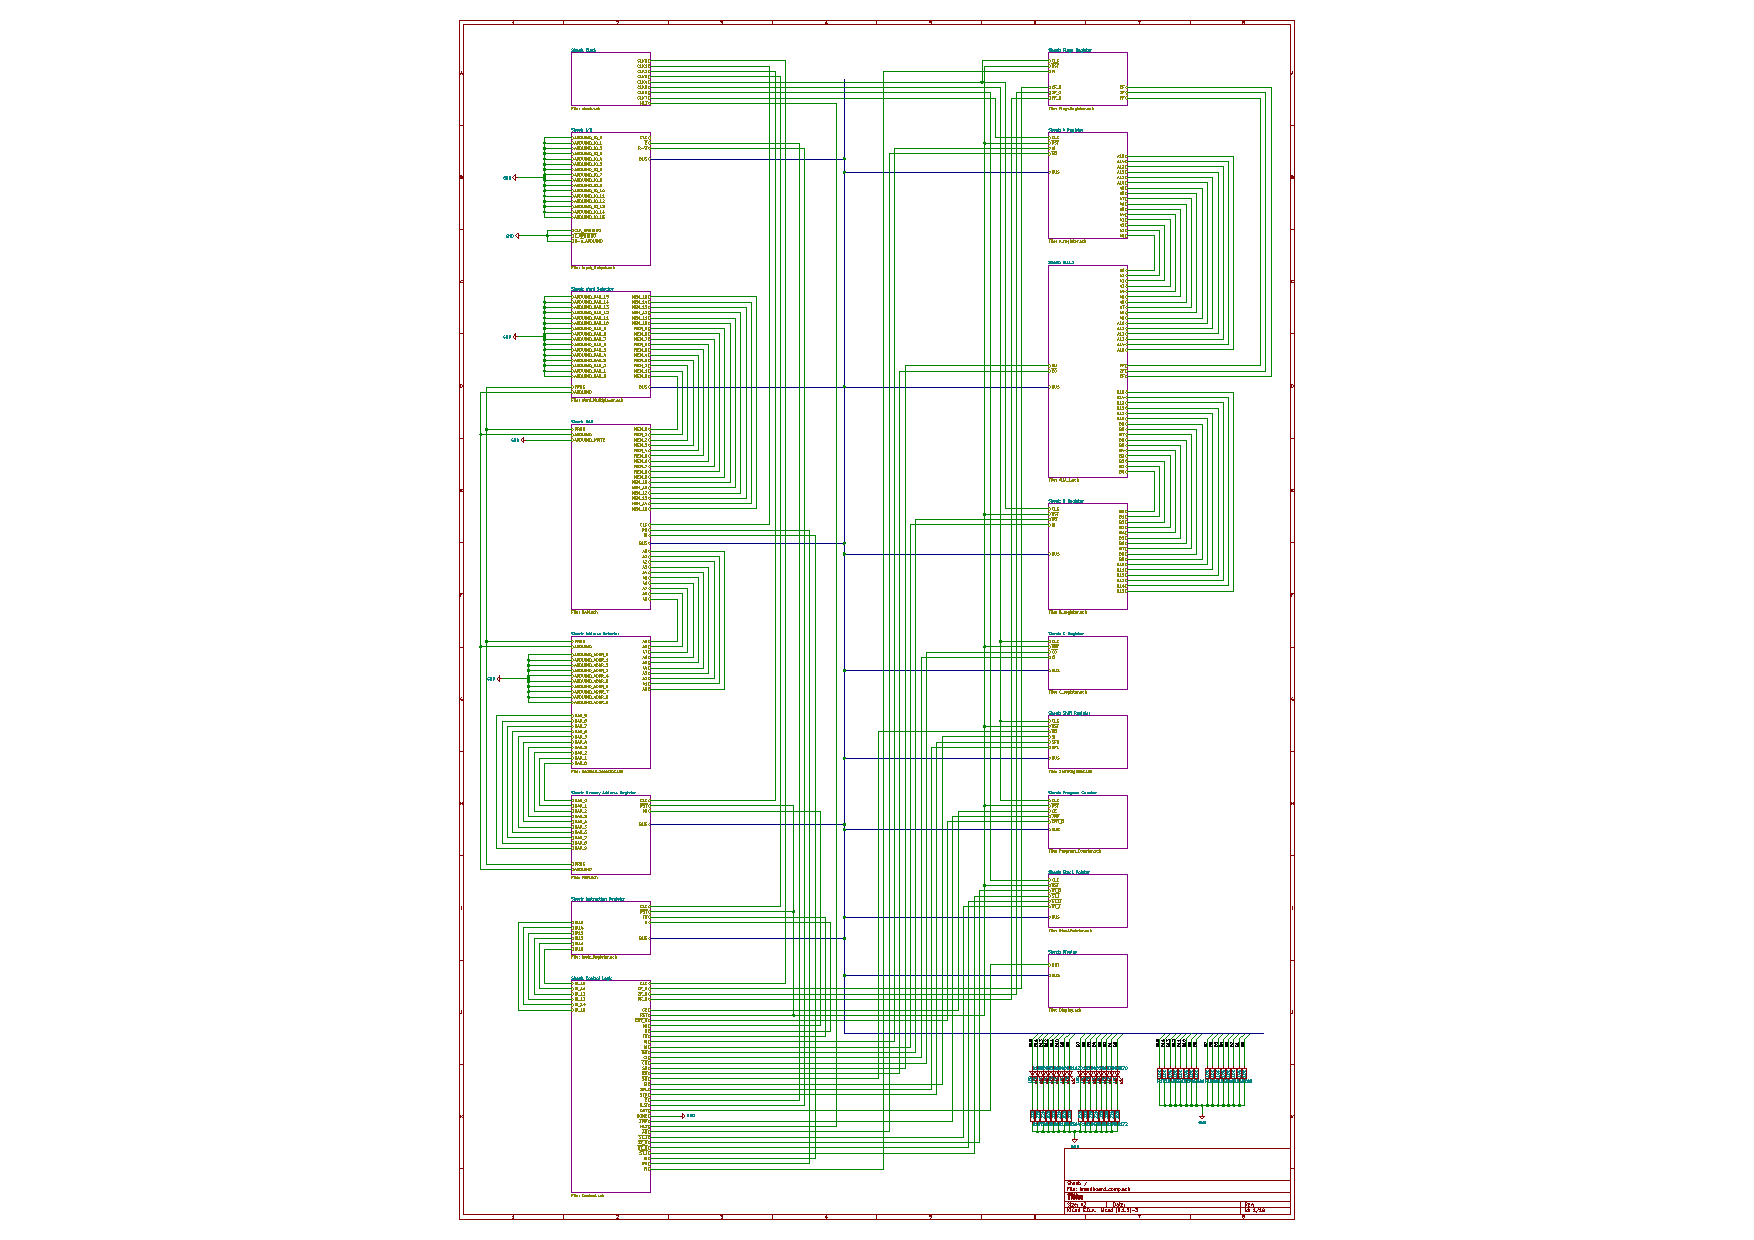
\includepdf[page={11}]{./pdf/kicad}

\paragraph{C Register} \ref{c-reg}
The C register is a general purpose 16-bit register built just like the A register \ref{a-reg} or the B register \ref{b-reg}.

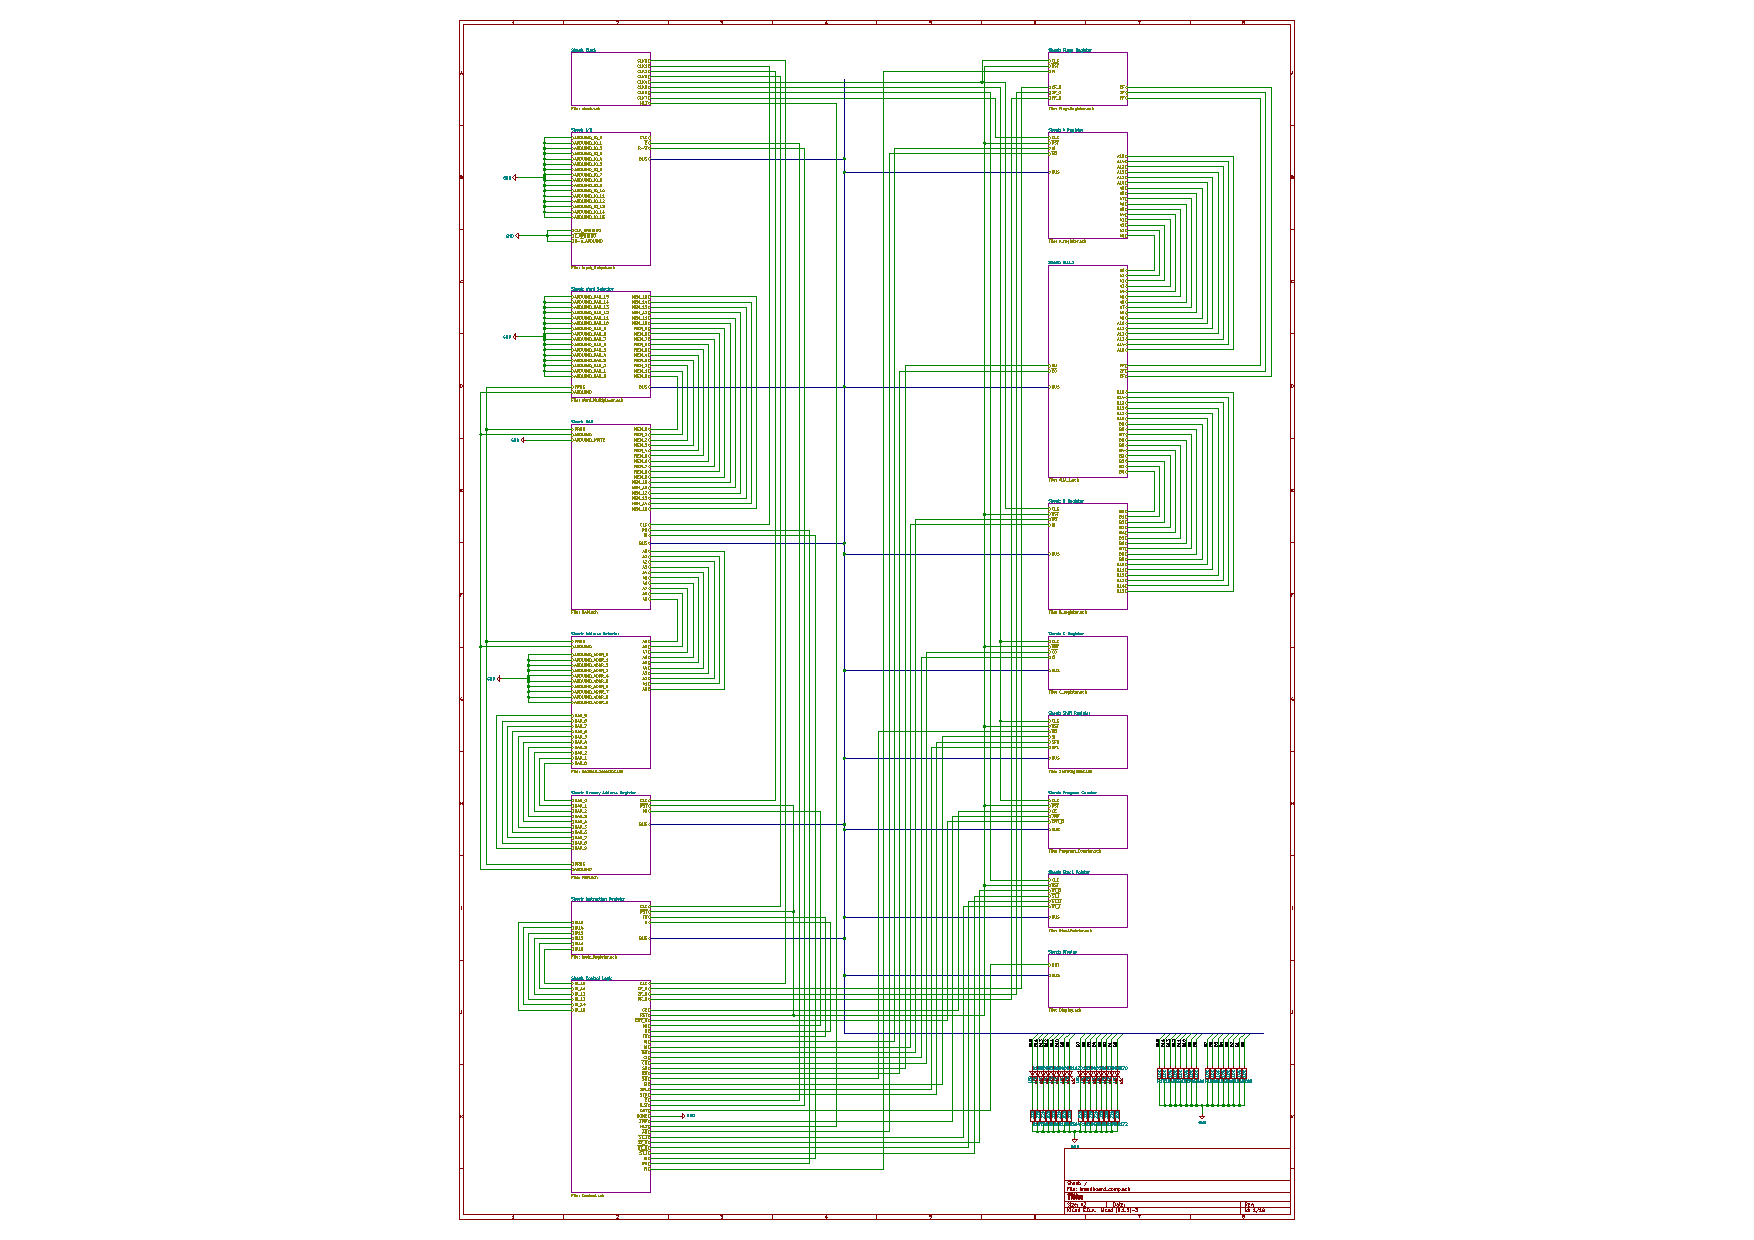
\includepdf[page={7}]{./pdf/kicad}

\paragraph{Shift Register} \ref{shift-reg}
For the design of the shift register, the \emph{74LS194} \cite{74ls194} was chosen. It is a 4-bit register which implements
bit shifting in both directions. Multiple \emph{74LS194} chips can be chained together to create a larger shift register by
connecting the Serial-Left and Serial-Right inputs of one chip to the data outputs of the chips to its left and right.
The chips have two control inputs, \emph{S0} and \emph{S1}. If both inputs are low, the register will do nothing on the next clock
pulse. If S0 or S1 is high, but not both, then a shift-right or a shift-left will occur, depending on which input is high.
If both are high, then a parallel load will occur. The data outputs of each chips are connected two two \emph{74LS245}
\cite{74ls245} chips to provided the interface to the data bus. The two control inputs are fed in from a simple combinatorial
circuit which converts the three control signals, \emph{SI}, or shift register in, \emph{SFL}, or shift left and \emph{SFR}, or
shift right, into the two lines which connect directly to the register chips.

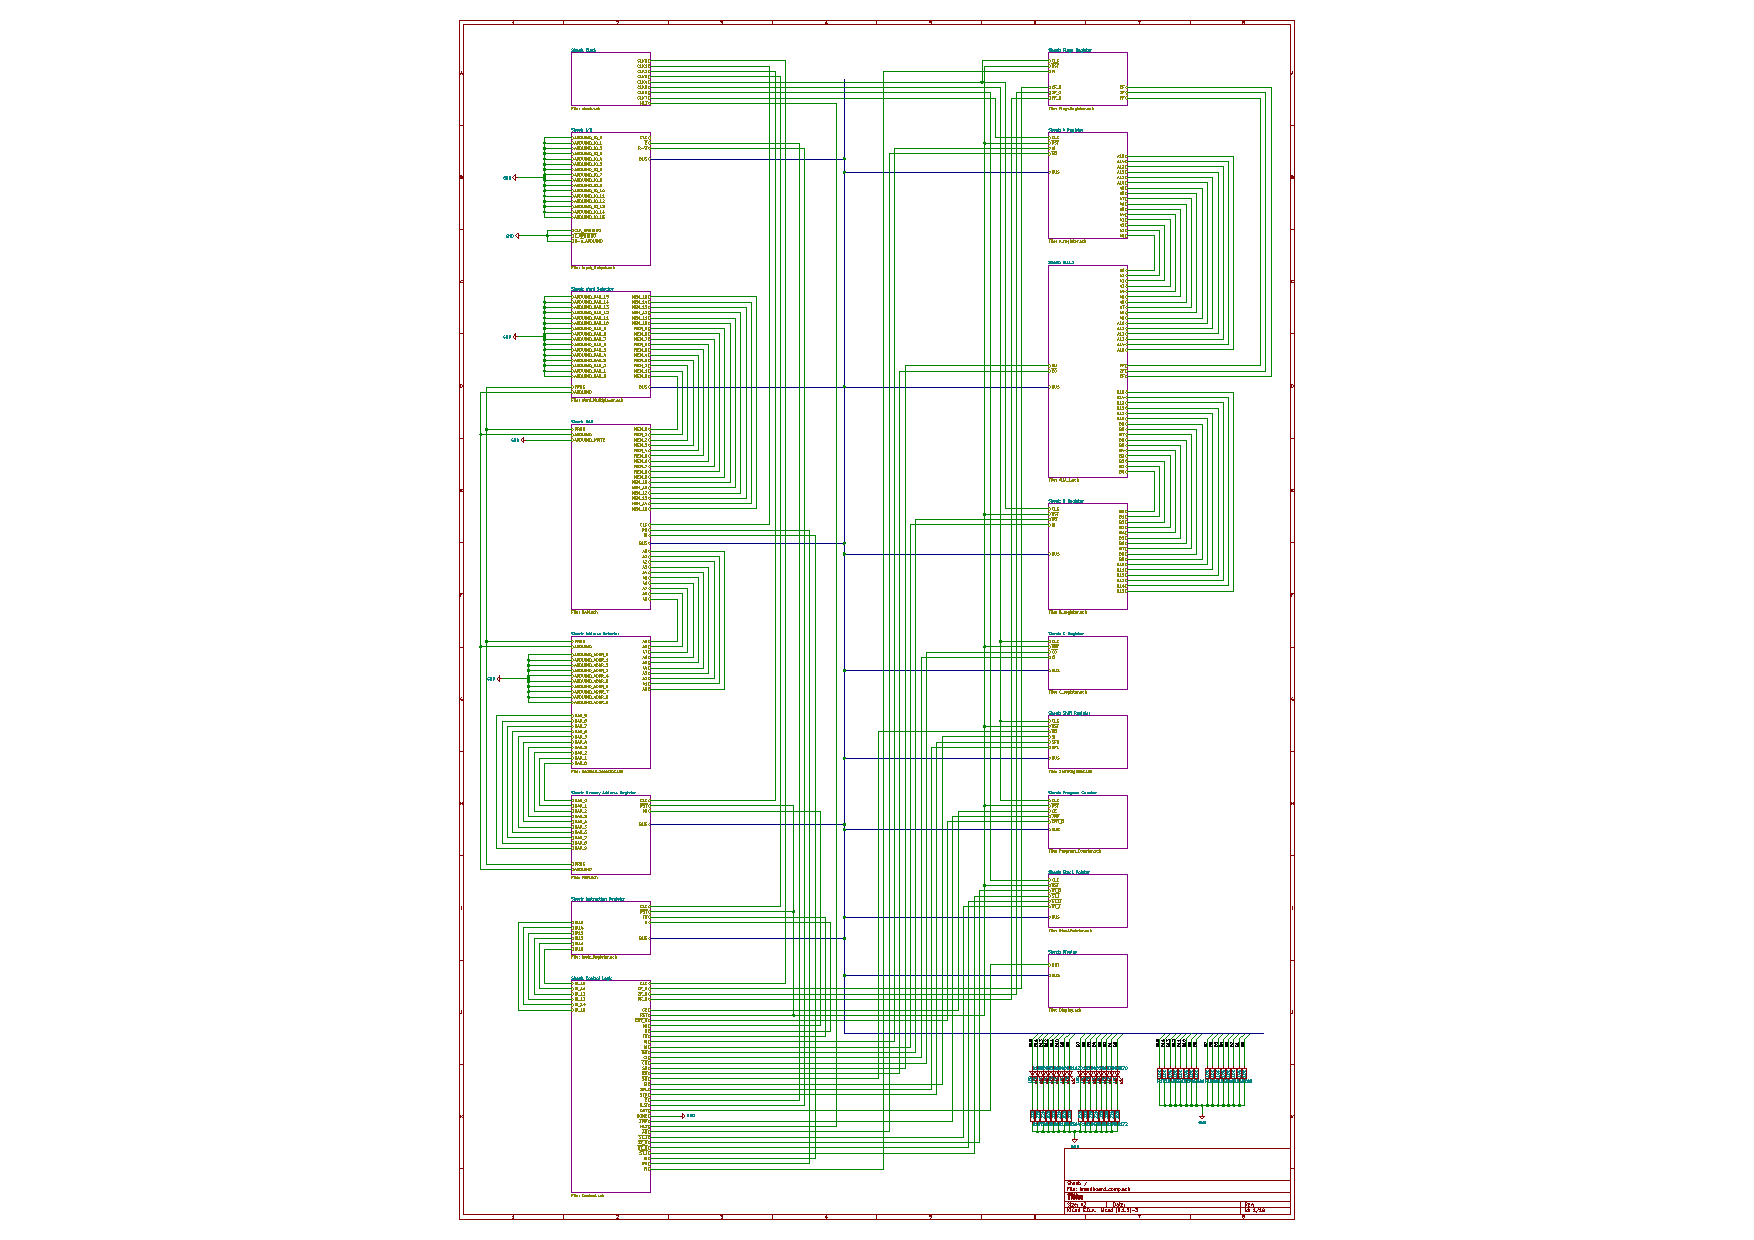
\includepdf[page={6}]{./pdf/kicad}

\paragraph{Random Access Memory (RAM)} \ref{ram}
The \emph{Random Acces Memory} module, or RAM module, poses an interesting design challenge. Thee \emph{7400} family of integrated
circuits does not include any circuits which would fulfil the 16K memory space specification previously chosen in a simple and
intuitive manner. As such, different chips had to be chosen. In the end the \emph{LY62256} 32K x 8-bit static RAM chip
\cite{ly62256} from \emph{Lynotek Inc.} and stocked by \cite{farnell} was selected. This chip was chosen because it provides
a sufficiently large address space as well as simple control inputs. Since the chips are not part of the standard symbol library,
a symbol had to be created for the \emph{LY62256} chips in the Symbol Editor. The chips have 15 address lines, too many for the
16-bit breadboard computer. This is not an issue though, as the extra lines, \emph{A10} through \emph{A14}, can be tied to logic
0 and ignored. \\
One chip stores one byte of data at any given address, so two chips were needed to adequately cover the entire 16K memory array.
Since the chips use the same pins for both data reads and writes, two sets of two \emph{74LS245} buffers \cite{74ls245}. In this
configuration, the data pins of each RAM chip are locked between two buffer chips and is, as such, effectivley isolated from the
rest of the computer. If reads a read operation is requested, the data bus facing buffers will activate and allow the data pins of
the RAM chips to drive the bus. If a write operation is requested, the word selector facing buffers will activate and allow data to
flow from the word selector to the RAM chip data pins. Besides this, some simple combinatorial logic is used to implement a selector
for the write \emph{RI} signal based on the \emph{ARDUINO} and \emph{PROG} signals.

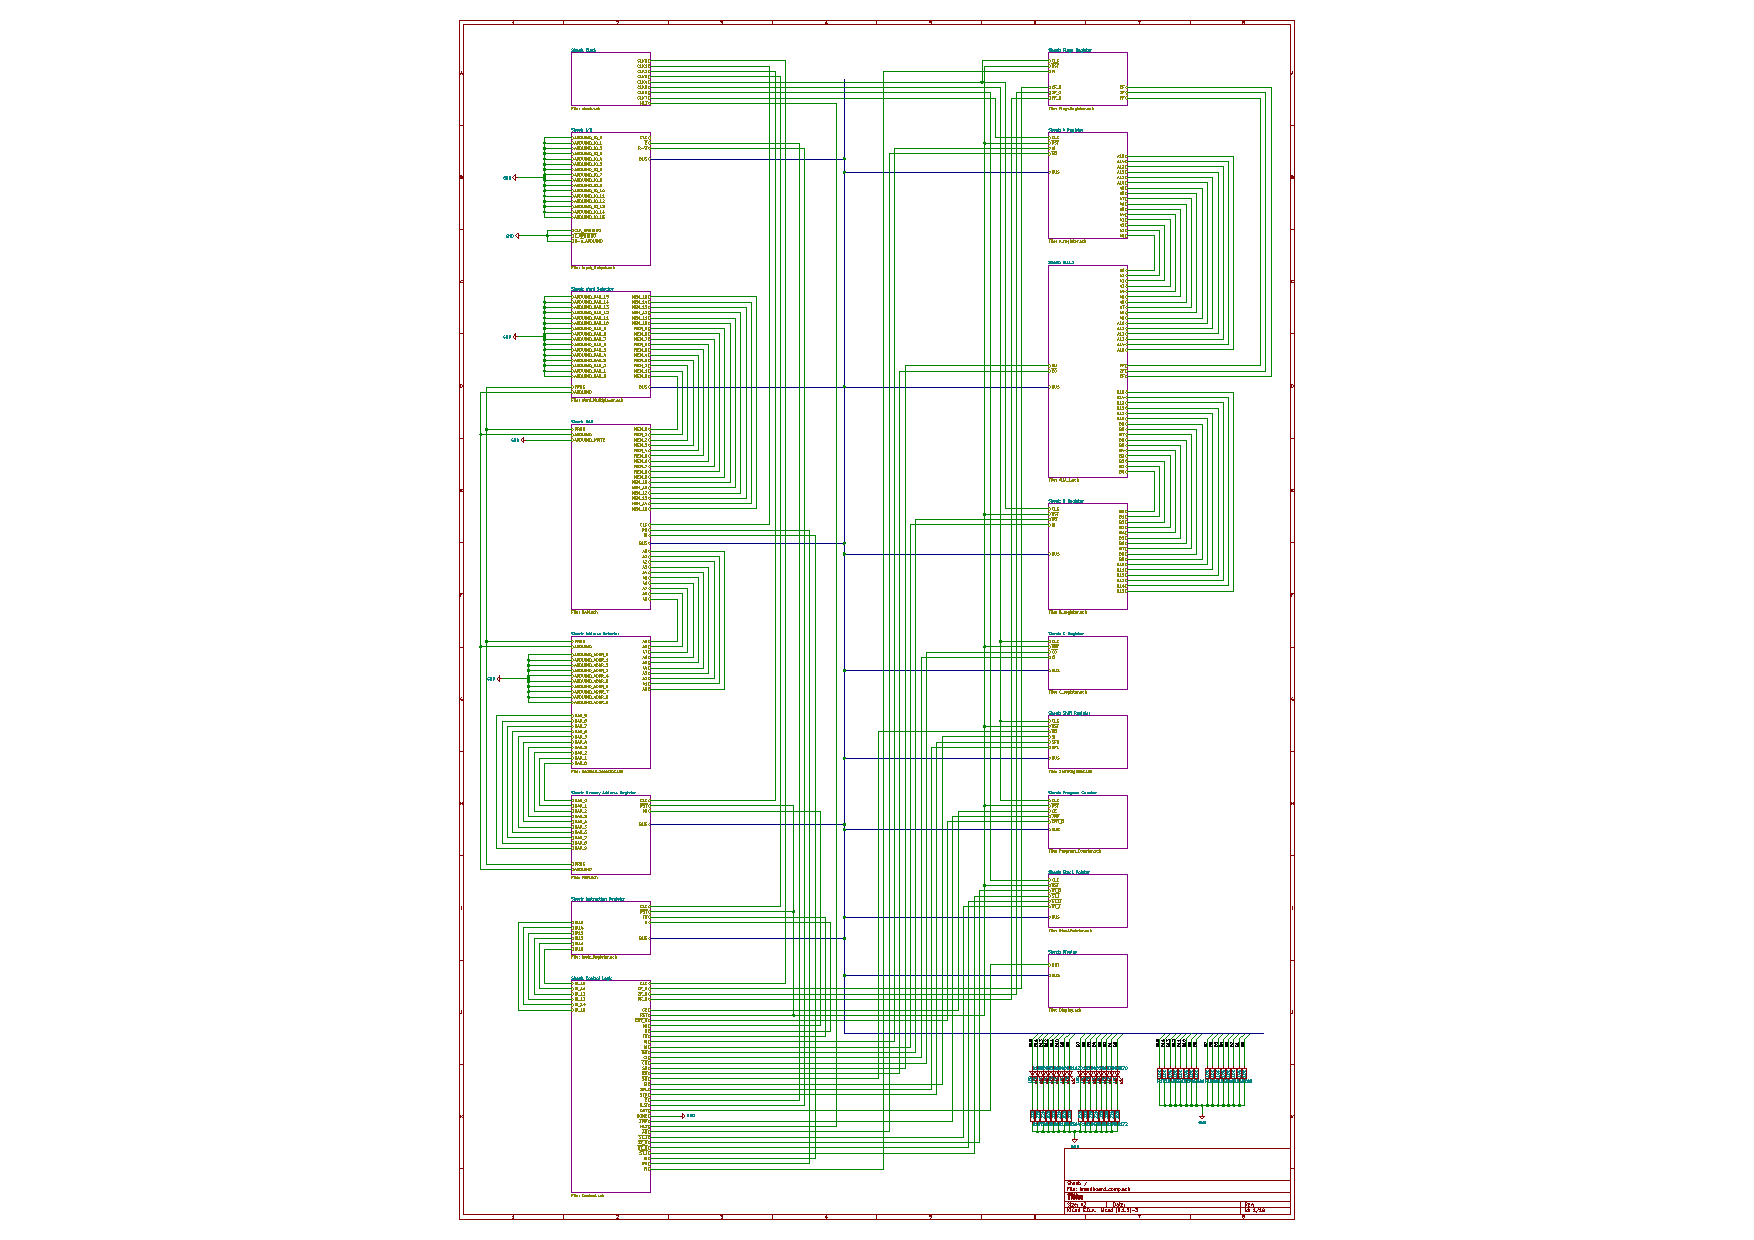
\includepdf[page={17}]{./pdf/kicad}

\paragraph{Program Counter} \ref{pc}
The centerpiece of the program counter module design is the \emph{74LS161} 4-bit binary counter \cite{74ls161}. This chips
implement most of the functionaility needed for the program counter. If the two enable signals are high, the chip will count
up in binary on the next clock pulse. If the \emph{Ripple Carry Output} pin is fed forward to the \emph{Enable T} signal of the
next counter, multiple counter can be used to create a binary counter of arbitrary length. In the case of the 16-bit breadboard
computer, to cover a 1K address space 10 bits are needed. This translates to three counters. Since the most significand two bits of
the most significand counter are not needed, the Q2 pin can be integrated into the reset circuit, so that the counter loops back
to 0 after reaching \emph{0x3FF}. Besides this, by having a parallel load pin, the \emph{74LS161}  facilitates jump functionailty,
used for programming branch and loop instructions. As usual, the bus interface is handled by two \emph{74LS245} \cite{74ls245}
chips. Since only 10 bits are connected from the counter chips to the buffers, the remaining six bits are tied low.
The control signals are decoded using simple combinatorial logic.

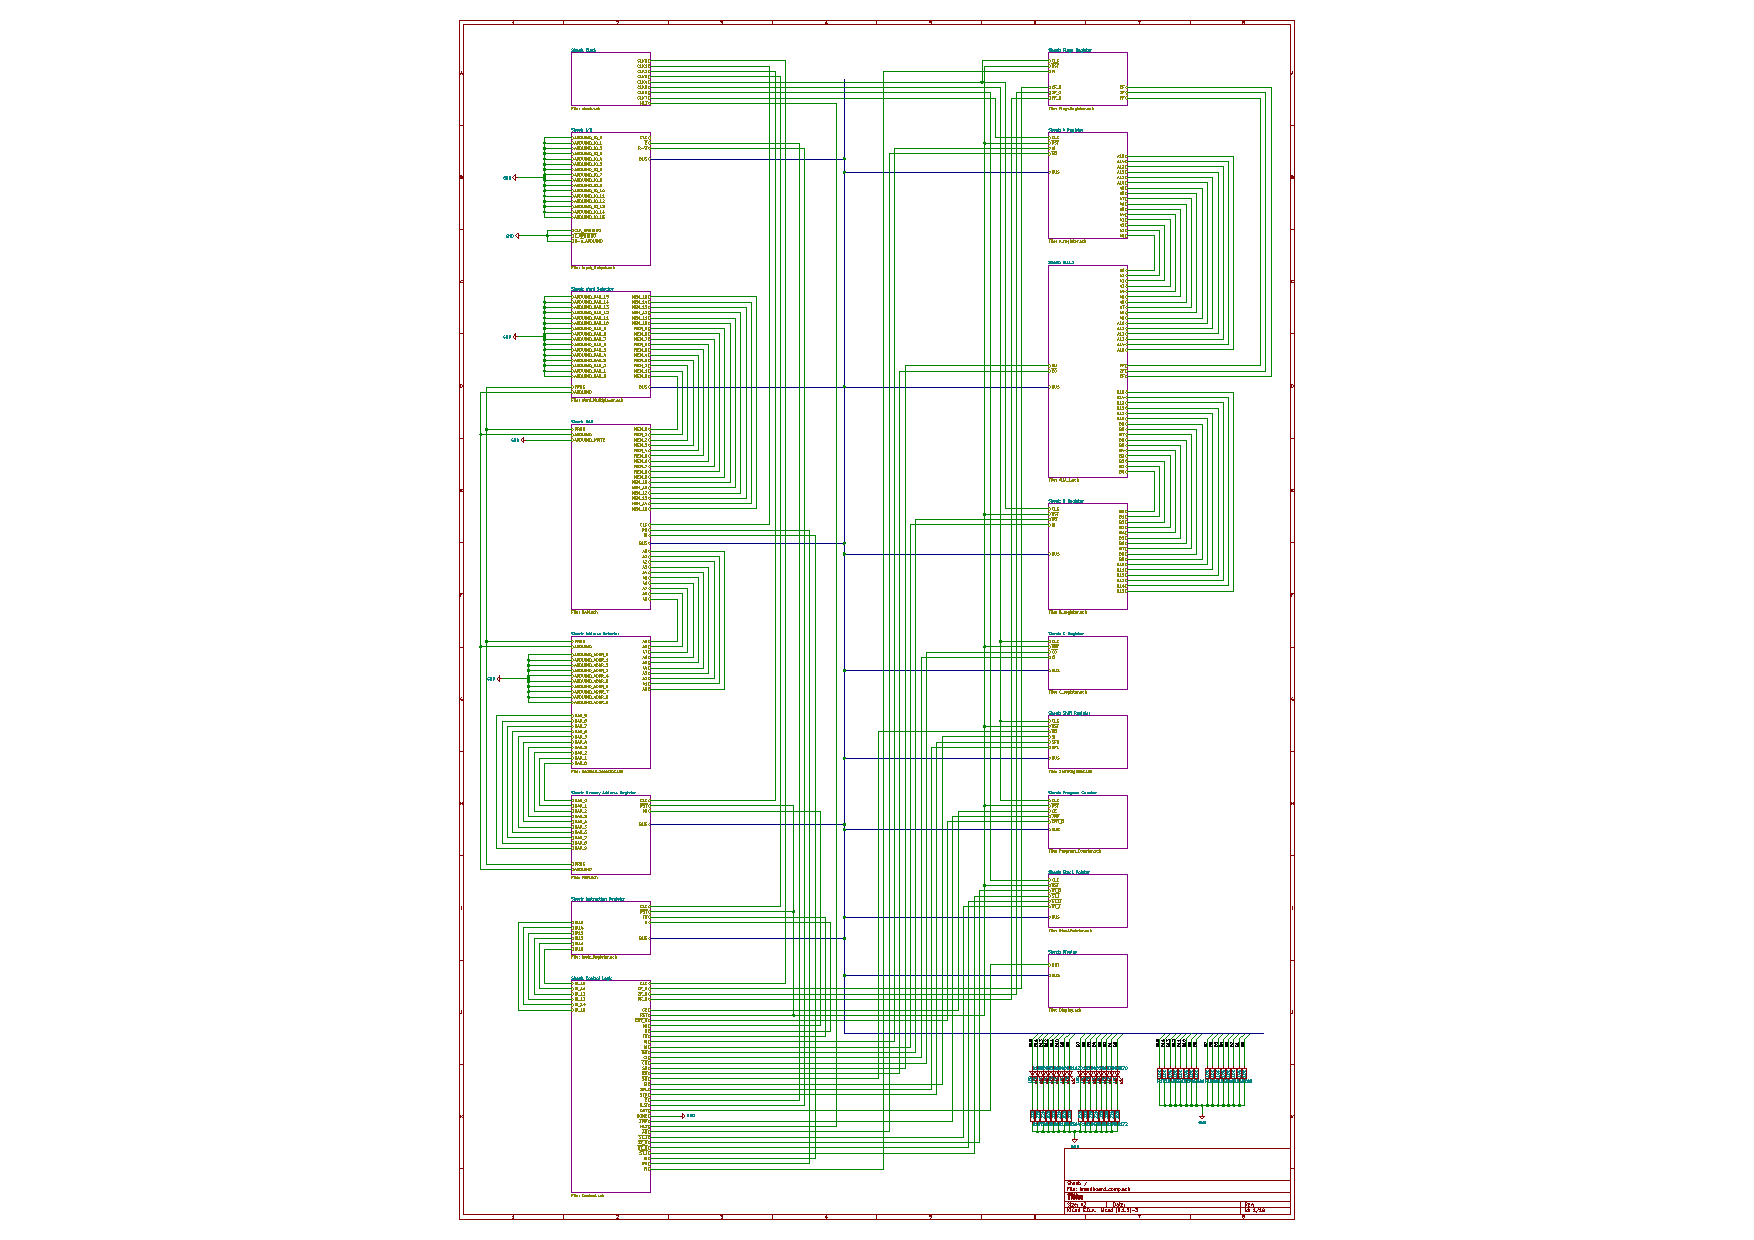
\includepdf[page={10}]{./pdf/kicad}

\paragraph{Stack Pointer} \ref{stack-pointer}
The stack is designed using a \emph{74LS169} 4-bit binary up-down counter chip \cite{74ls169}. Allthough limited,
the chip fits the specification because only a small fraction of the address space is alloted to the stack. The stack is formed
of the last 16 addresses, so only 4 bits are needed to specify them, since the remaining 6 bits are identical for all stack
addresses. The \emph{74LS169} differs from the \emph{74LS161} \cite{74ls161} used in the Program Counter \ref{pc} in the fact that
it trades in the master reset pin with the up-down pin, which controls which way the counter counts. As such, to preserve reset
functionality, a \emph{74LS157} \cite{74ls157} multiplexer chip is used. This chip selects between two sets of 4 bits based on
the state of a single control bit. This is used in the stack pointer for loading in either the lowest significant four data bus
bits, in case a stack jump is to be executed, and 4 low values, in case a reset is to be executed. This restores the missing
reset functionality. Besides this, two \emph{74LS245} \cite{74ls245}  chips are used to interface to the bus. Besides the four
bits provided by the stack pointer, the next six bits are tied to logic 1, to reflect the position of the stack address range in
the memory space. The rest are tied to logic 0. Finally, some simple gate logic manages the control signals.

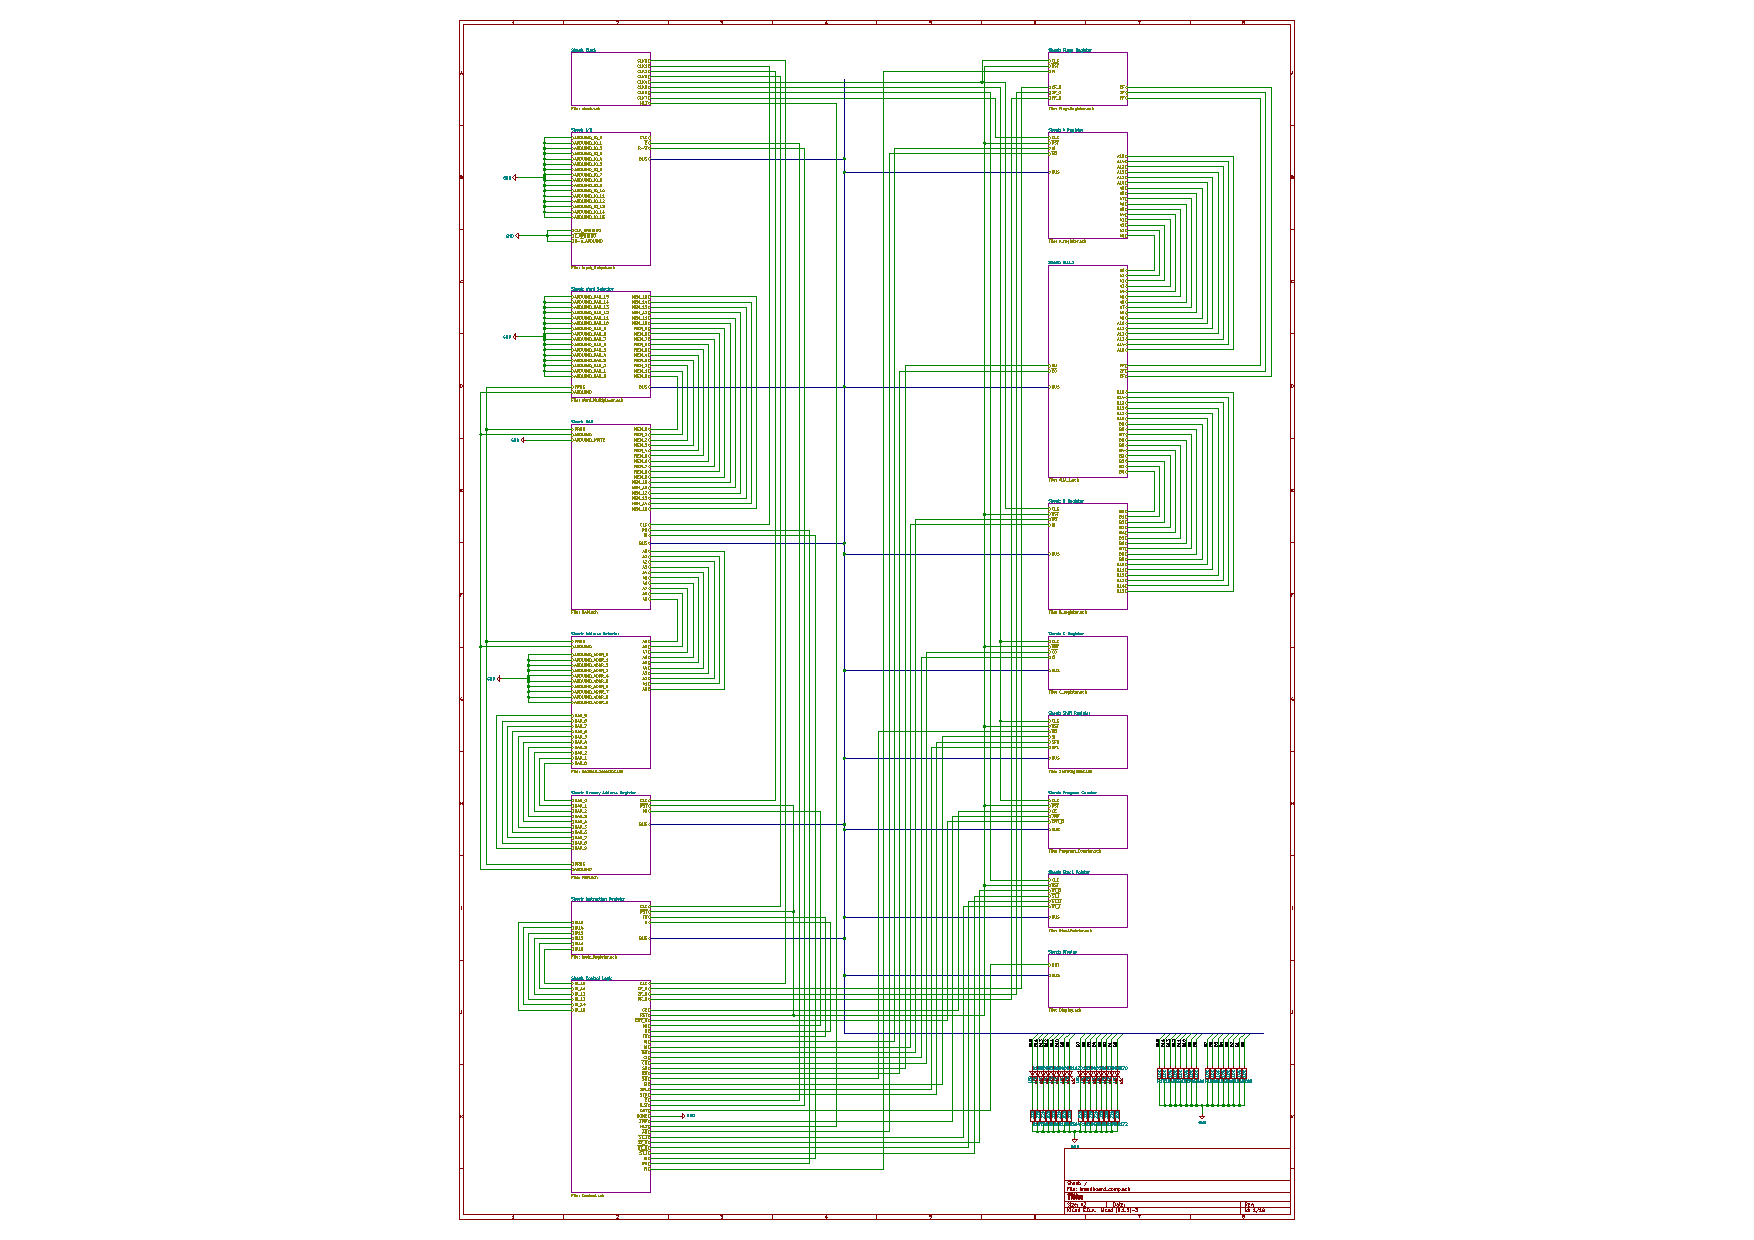
\includepdf[page={14}]{./pdf/kicad}

\paragraph{Display} \ref{display}
To fit the specification of a 16 characters by two line display, while maintaining relative simplicity, the \emph{c1602a v1.2}
\cite{c1602a} was chosen. This simple and widley popular LCD modules are easy enough to use and abstract a sizable amount of the
issues with character generation and display, so that a single person can master them in a relativley short span of time. They have
an internal character set and also allow the user to specify as small set of custom characters. To interact with the
\emph{c1602a v1.2}, a word of 9 bits is sent to the display on the rising edge of the \emph{Out} signal. The first bit
specifies wheter a command or a character is sent to the display, and the remaining byte represents the command or the character.
The display also implements functionailty which allows the main processor to read data from it, but this will be abstracted away,
as it is not part of the specification. Besides the data and \emph{Out} signal, the \emph{c1602a} requires just power connection
for the processor and backlight, as well as a variable resistor for the adjustable contrast.
Besides the display, two \emph{74LS245} buffer chips \cite{74ls245} are used to interface the display to the data bus. That being
said, only the least significand 9 data bits pass trough the buffer to the display, as that's all that is required.

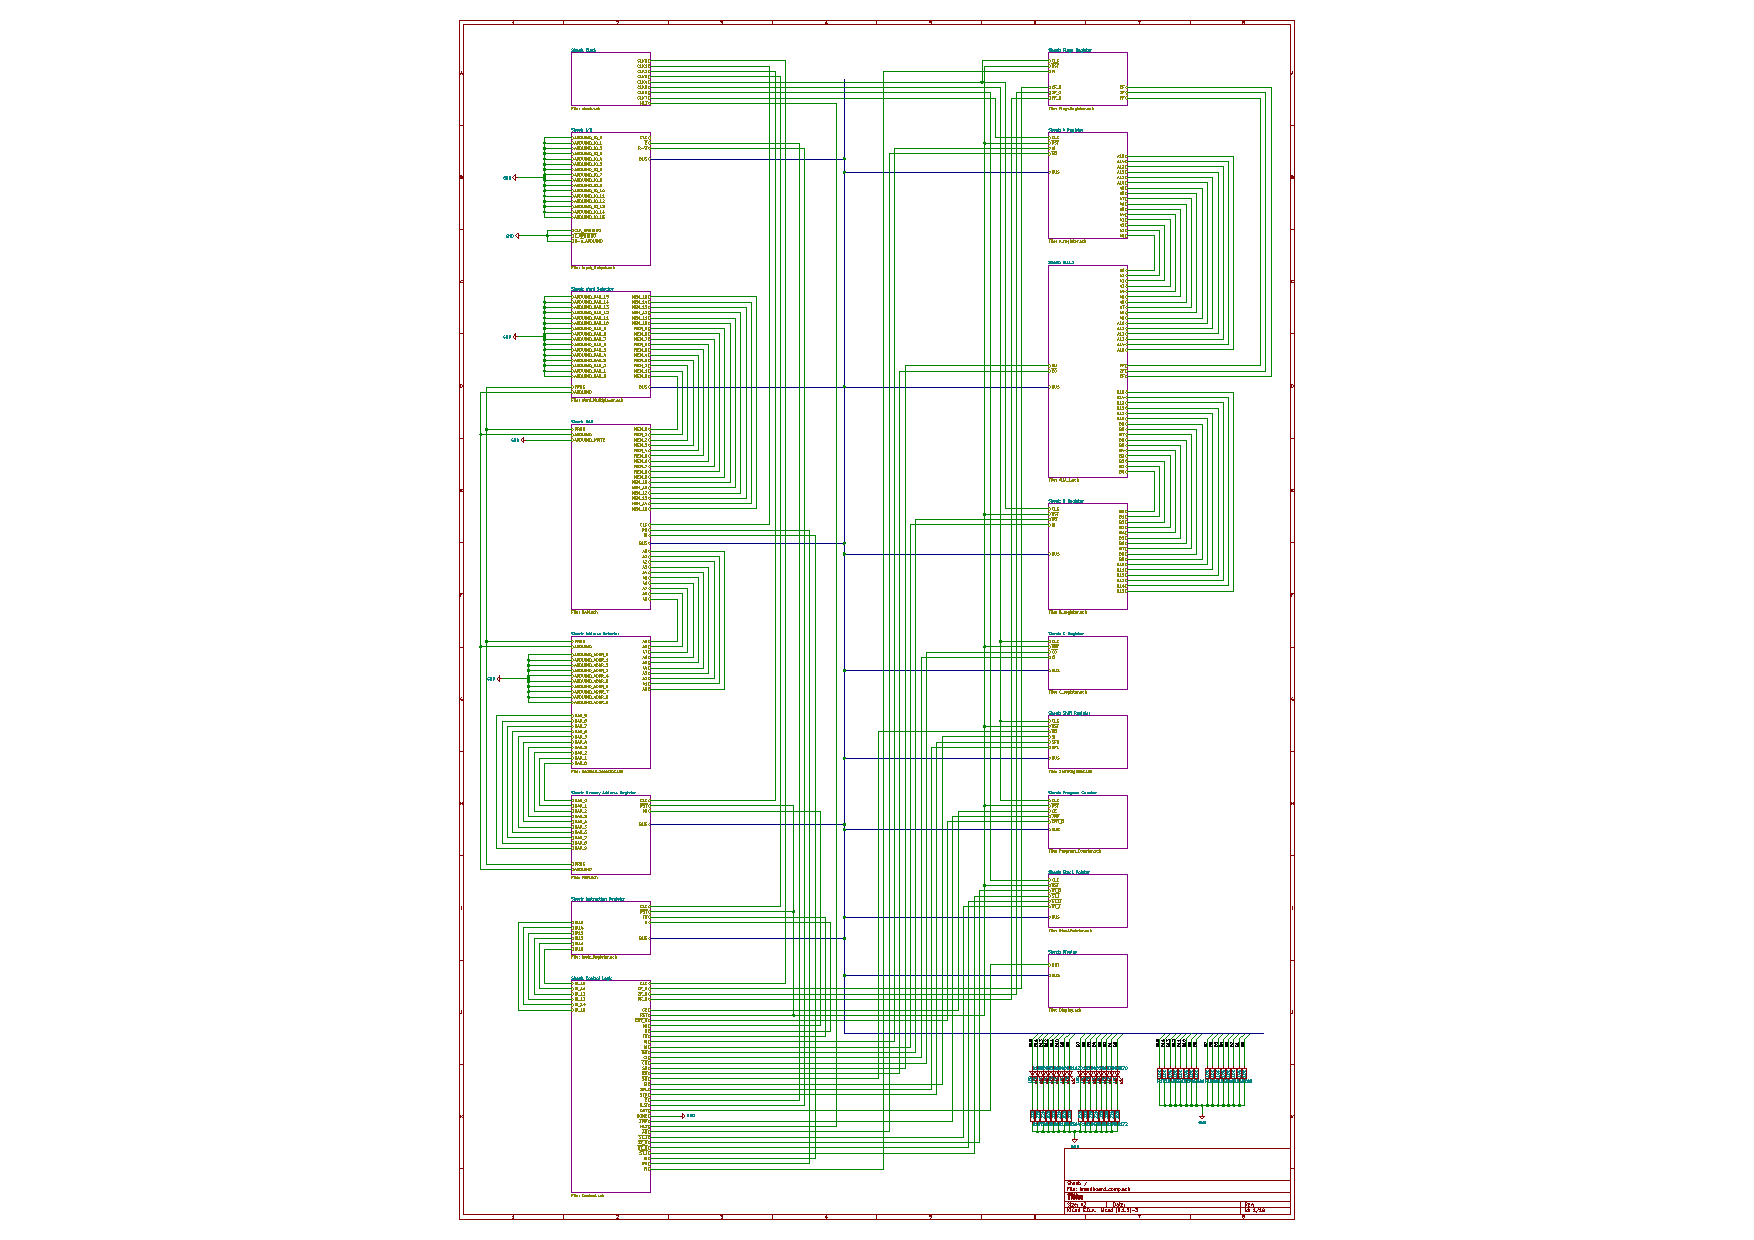
\includepdf[page={12}]{./pdf/kicad}

\paragraph{I/O} \ref{io}
The I/O module provides outside connective to an \emph{Arduino Mega} \cite{arduino2020mega}. To achieve this, two \emph{74LS245}
\cite{74ls245} buffer chips are used. When the buffers are disabled, the  Arduino and the main system are essentially
disconnected. This ensures that there is no interference when no I/O requests are issued. Furthermore, the buffers are
actually bi-directional, so by means of the \emph{Read/Write} control signal, the computer can control if data flows from
the data bus to the arduino in case of an I/O write, or the other way around in case of an I/O read. The arduino can use the
\emph{Enable} signal to trigger an interrupt and handle the I/O request and the same \emph{Read/Write} to decide what the type
of the I/O request is and handle it accordingly.

 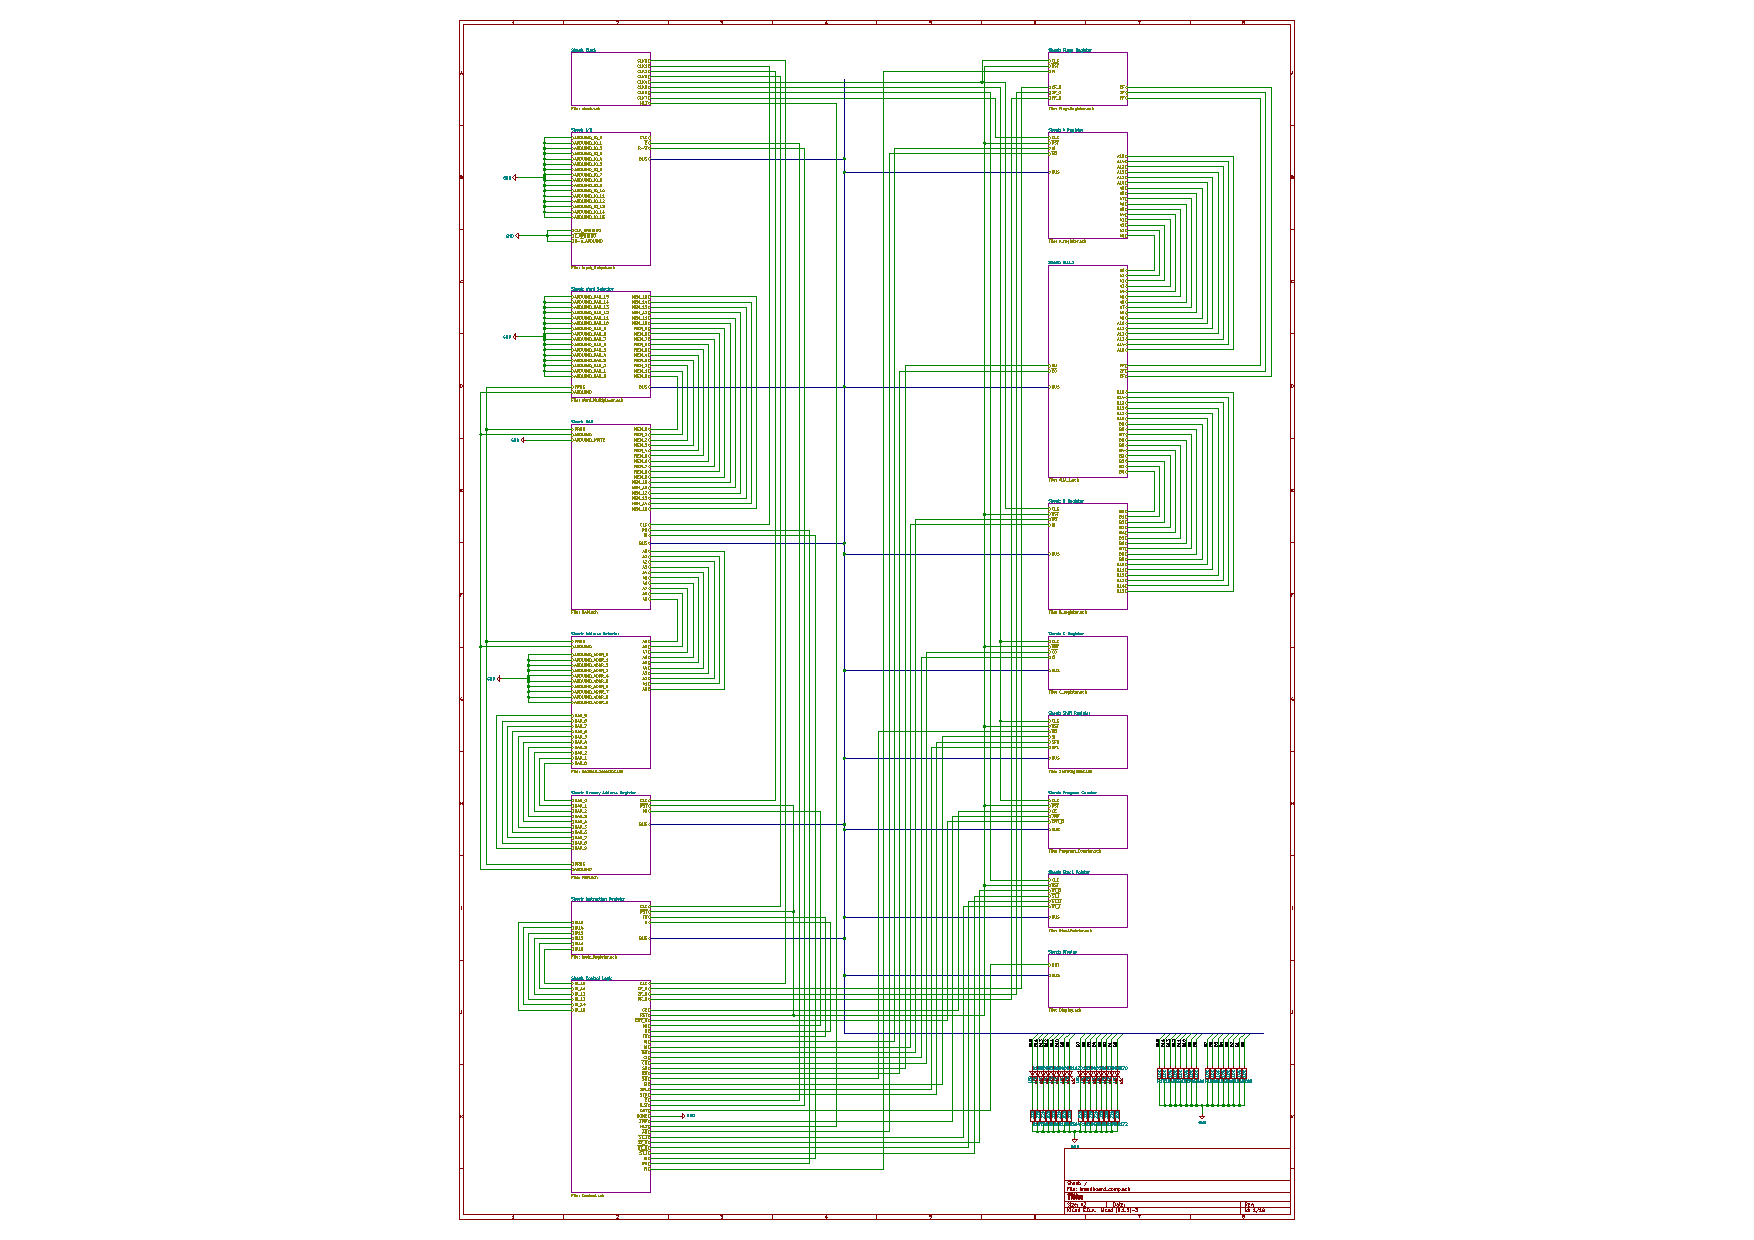
\includepdf[page={13}]{./pdf/kicad}

 \paragraph{Memory Address Register} \ref{mar}
 To design the memory address register, the same chips which was used in the A register \ref{a-reg}, the B register \ref{b-reg},
 the C register \ref{c-reg} and the flags register \ref{flags}, namely the \emph{74LS273}
 \ref{74ls273}, comes to mind. Since the memory address register will not assert its contents to the bus, there is no need for
 a data bus buffer. But, since the module is built up of few components and is placed in the vicinity of RAM \ref{ram} and the
 address selector \ref{addr-select}, it lends itself as a good location for the two toggle switches which will be used to
 set the \emph{ARDUINO} And \emph{PROG} control signals.

 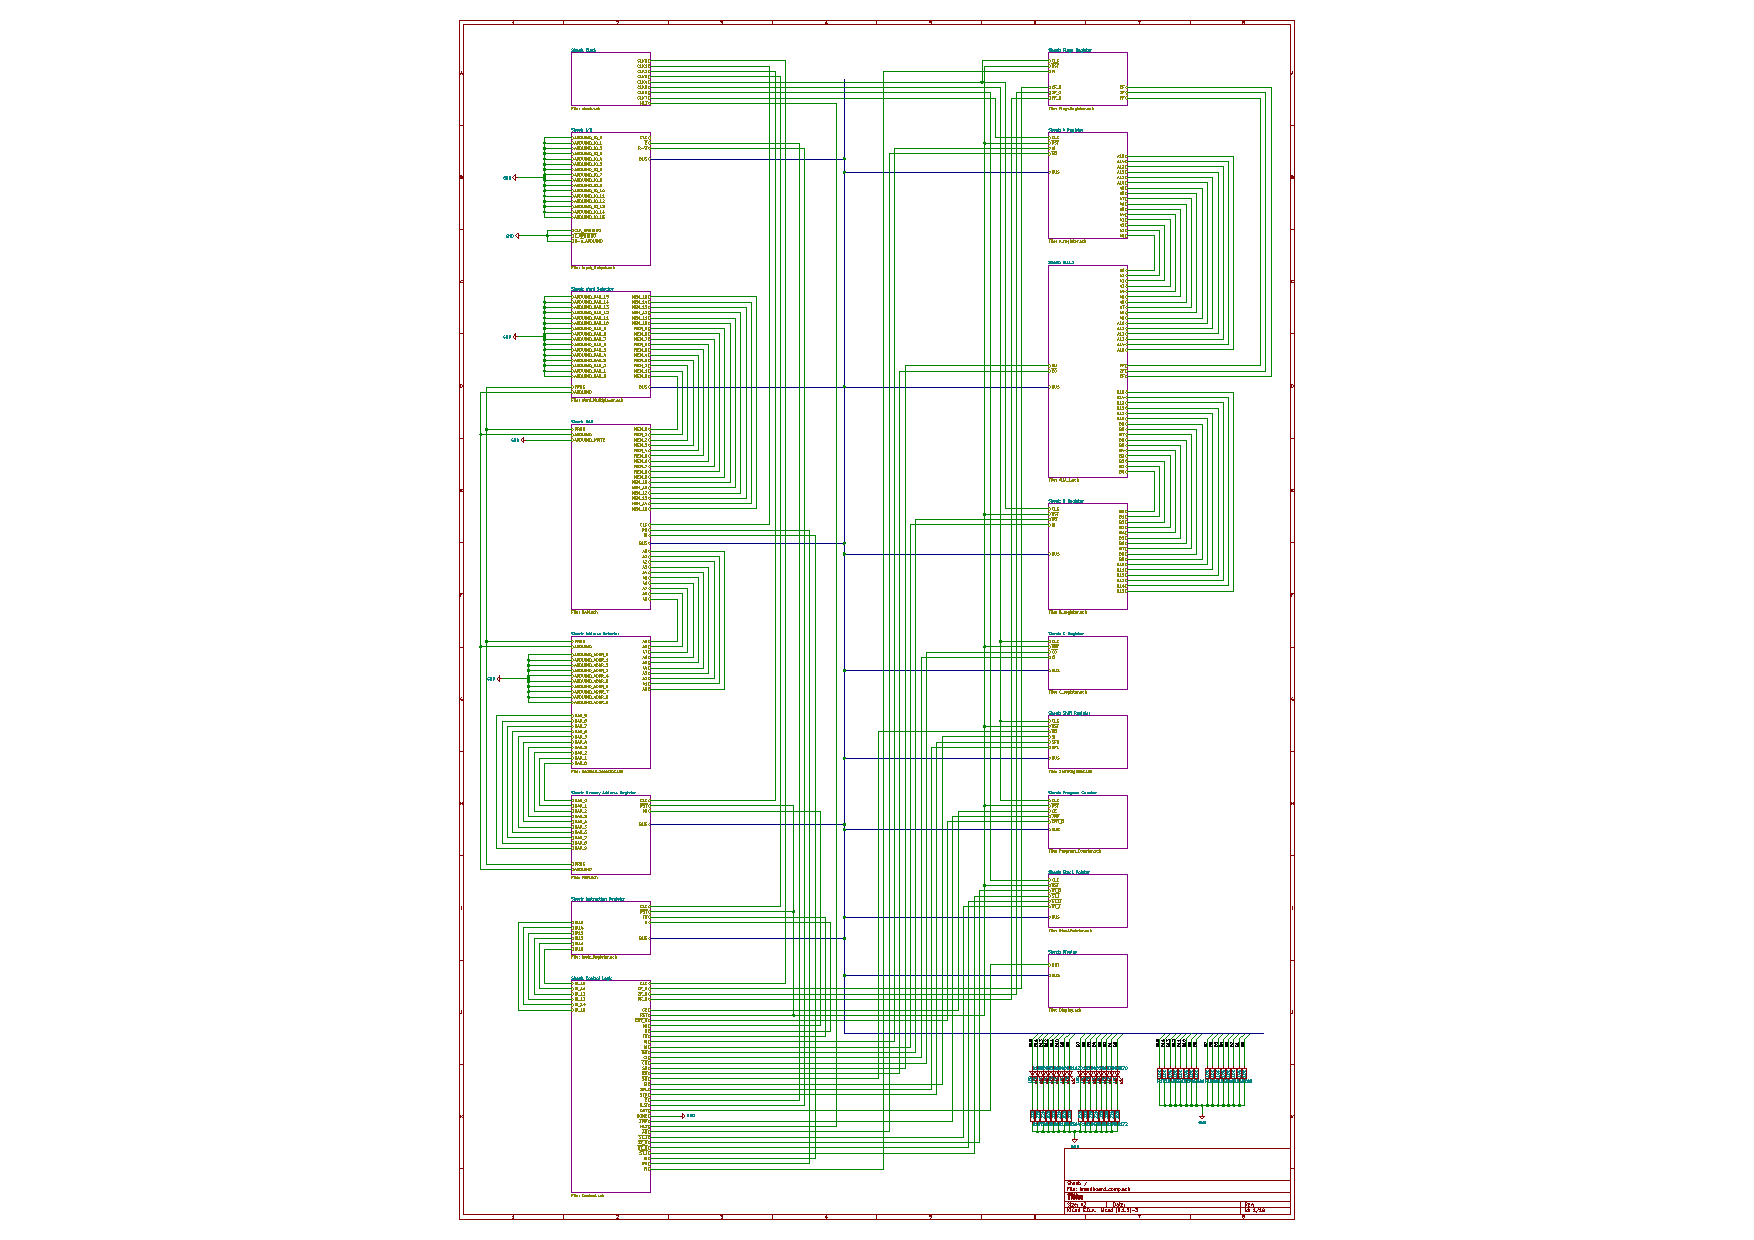
\includepdf[page={9}]{./pdf/kicad}

 \paragraph{Instruction Register} \ref{ir}
 The instruction Register is very similar in construction the the A register \ref{a-reg}, B register \ref{b-reg} and C register
 \ref{c-reg}. It uses two \emph{74LS273} \cite{74ls273} 8-bit flip-flop chips to store one 16-bit word of data, which can be
 latched in from the data bus. It also has two \emph{74LS245} buffer chips used to assert its contents onto the bus when a read
 request is issued. The main difference between the Instruction Register and any other register is the fact that only its 10
 least significand bits are asserted back onto the data bus during a read operation. This is because the Instruction Regsiter
 holds instructions, which are structered as a six-bit \emph{opcode} and a 10-bit \emph{address or immediate operand}. The 6-bit
 \emph{opcode} is connected directly to the \emph{control logic} module. Control Signal processing is handled using a simple
 AND gate.

 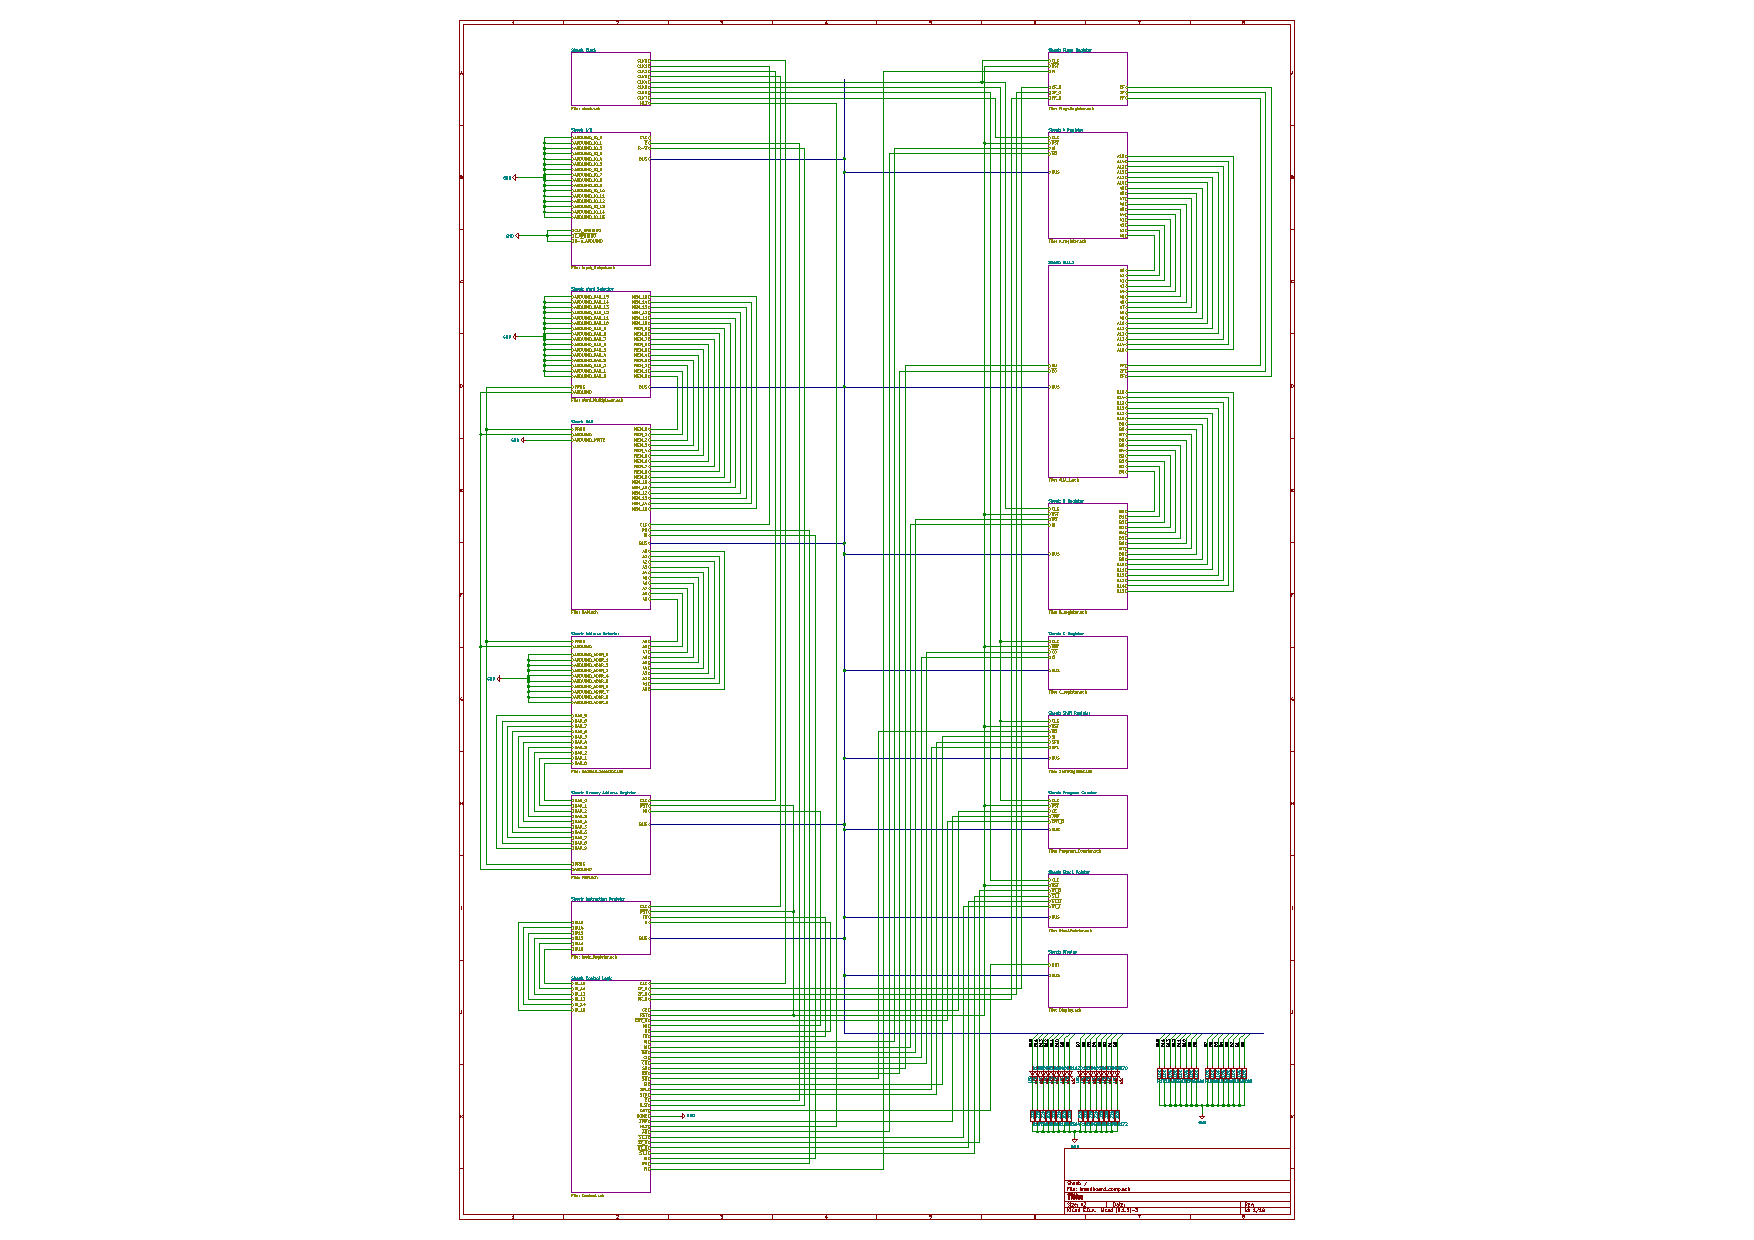
\includepdf[page={18}]{./pdf/kicad}

 \paragraph{Word Selector} \ref{word-select}
 The Word Selector design heavily relies on the \emph{74LS157} data selector chip \cite{74ls157}. A two stage design is proposed.
 The first stage of four selector chips chooses between the data provided by the /emph{DIP switches} and the \emph{Arduino Mega}
 \cite{arduino2020mega}. This stage is handeled by the \emph{ARDUINO} control signal. The output of this selector stage is fed
 forward to the second stage of 4 selector chips. These chips decide wheter to output the programming data provided by the
 previous selectors or the bus data based on the \emph{PROG} signal.

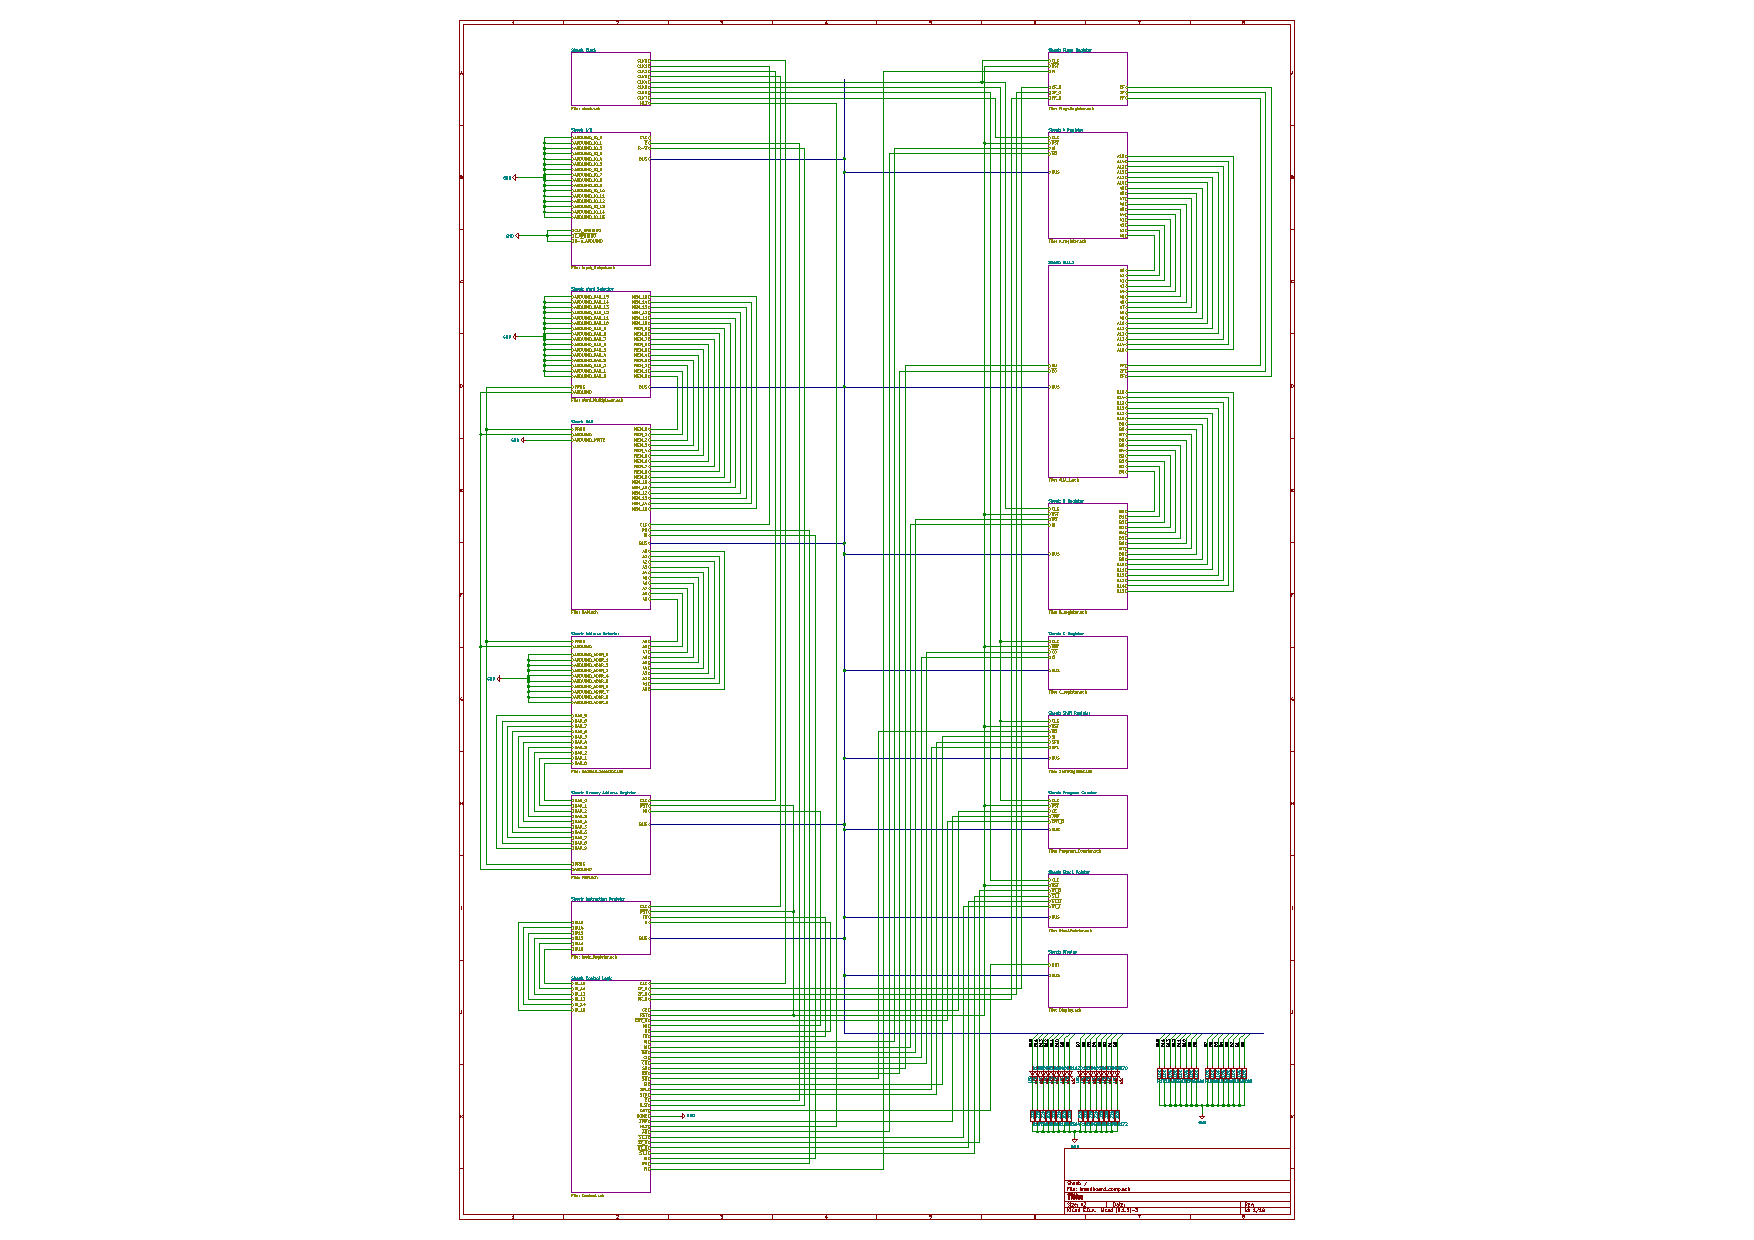
\includepdf[page={15}]{./pdf/kicad}

\paragraph{Address Selector} \ref{addr-select}
The Address selector is designed the same way as the Word Selector described in the previous
paragraph. The main difference is that, since it only has a final output of 10 bits,
each selector stage only contains three \emph{74LS157} \cite{74ls157} selector chips.

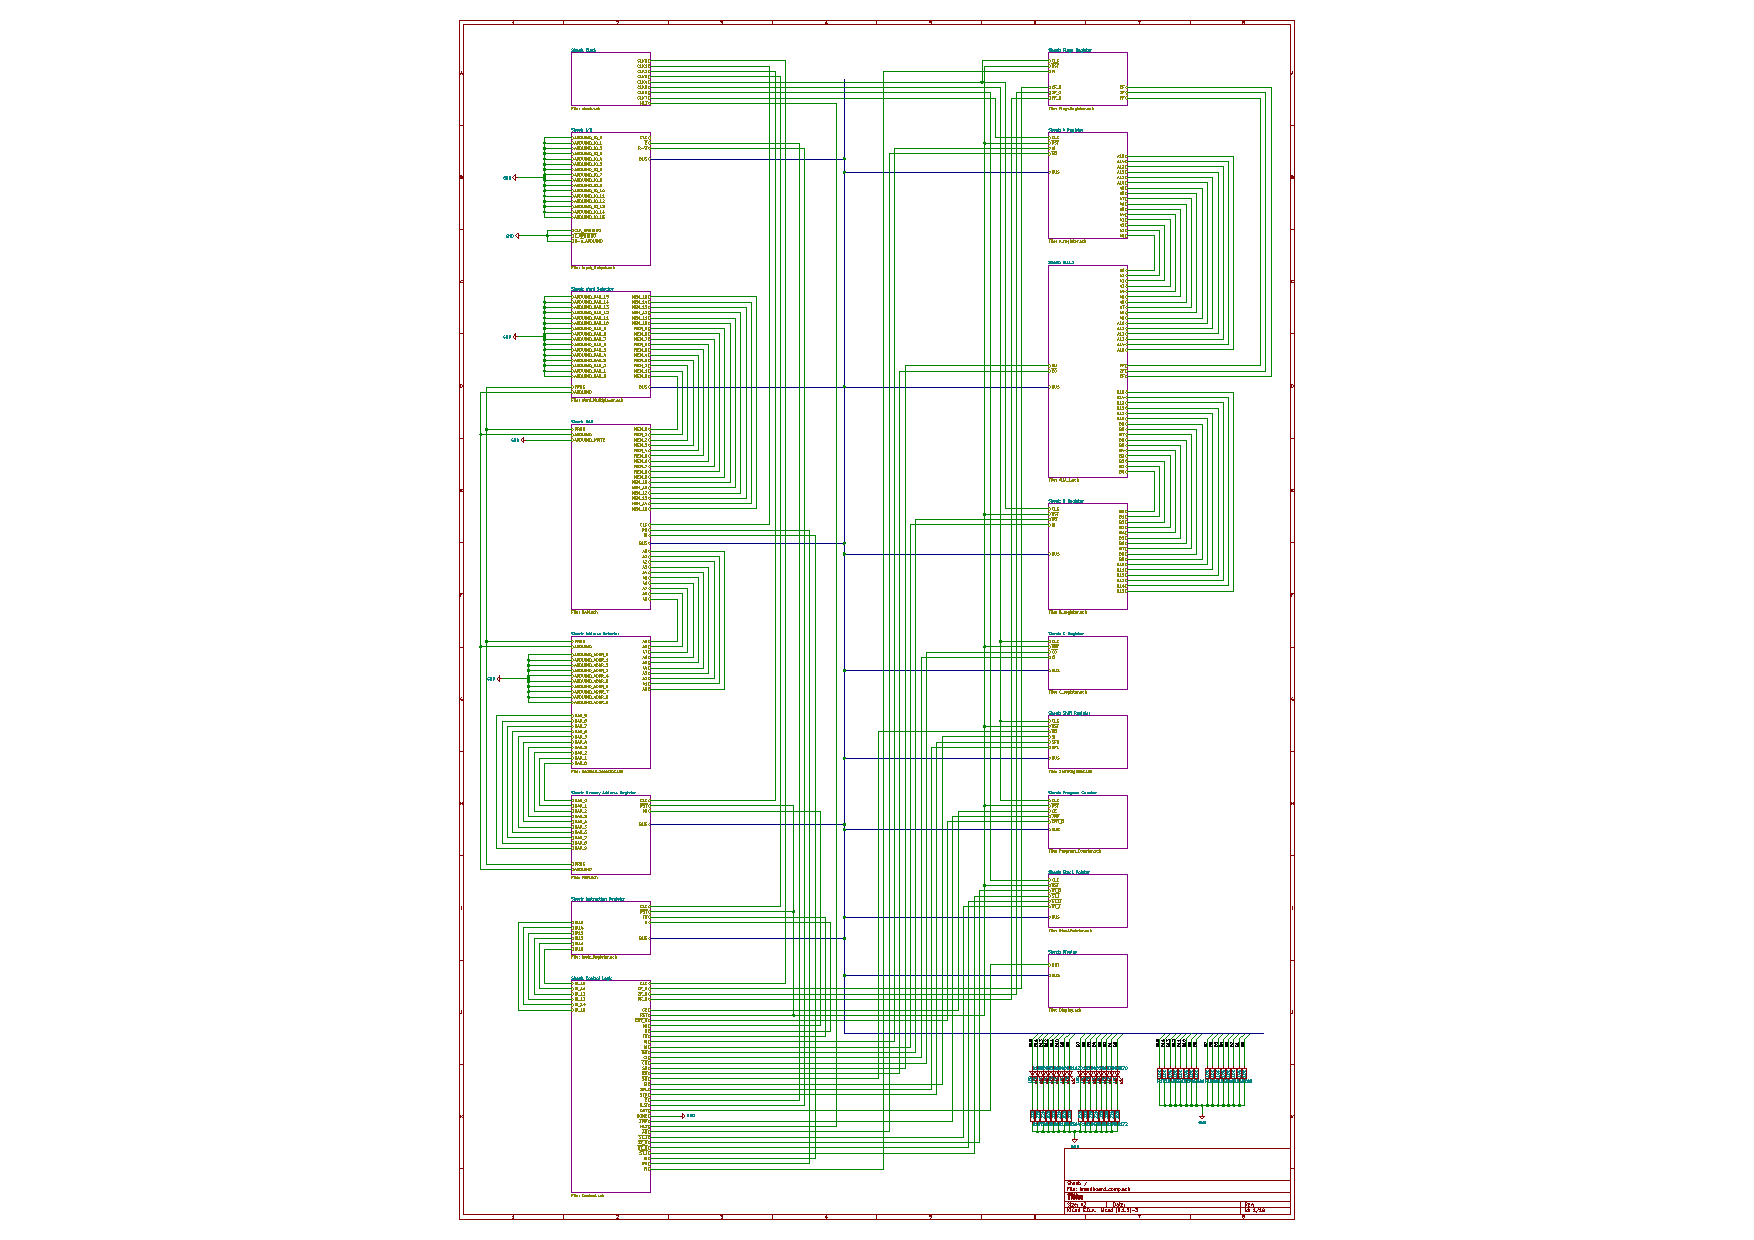
\includepdf[page={8}]{./pdf/kicad}

\paragraph{Control Signals}
The design of the Control Logic module \ref{control-logic} is centered around the \emph{AT28C64B}
EEPROM chip from \emph{Atmel} \cite{at28c64b}. EEPROM stands for \emph{Electronically Erasable
and programmable Read-Only Memory}. Essentially, an EEPROM memory acts as a look-up table.
It's input is an address and the output is a word of data. This can be used as a substitute
for any combinatorial circuit made out of ANDs, ORs, inverters etc.. By choosing an EEPROM,
instead of building a combinatorial circuit, the completed design benefits from multiple
advantages:
\begin{itemize}
  \item \emph{Simplified design:} if a combinatorial circuit would be designed in the place of
  EEPROMS, it would be of a significant size, given the large number of variables (10 binary
  inputs and 31 binary outputs). Such a circuit would not only be very dificult to design and
  physically implement with chips and wires, it would also go against the core design principle
  of simplicity of understanding.
  \item \emph{Easy re-progamming:} EEPROMs can be re-programmed using an of-the-shelf USB
  programmer, a microcontroller like an Arduino \ref{arduino2020mega} or even a simple custom
  built circuit. This makes them especially suitable for application in the design of 16-bit
  breadboard computer as they can easily be removed from the module, reprogrammed to include
  new instructions or modify existing ones and then re-inserted into to rest of the circuit.
  \item \emph{No extra conceptual abstraction}: While the EEPROM chips themselves are much more
  complex chips compared to most of the chips used in other modules (their data sheet doesn't
  provide a transistor diagram or even a low-level diagram, just a high-level block diagram),
  conceptually they don't increase the complexity of the design, since they can be thought of
  as a combinatorial circuit made of simple gates or a memory array made up of rows of registers
  with a selection circuit. As such, the simplicity of both concept and physical implementation
  is maintained.
\end{itemize}
The reasons for choosing this particular EEPROM chip are as follows:
\begin{itemize}
  \item \emph{Parallel Interface: } There are two main types of EEPROMs: parallel and serial. A
  serial interface uses a single pin to transmit addresses and data respecitvley. This poses
  issue to the design of the module since a separate, faster clock and a shift circuit would be
  needed to shift in addresses and shift out data on each clock cycle. This significantly adds
  to the complexity of the entire design. A parallel interface, on the other hand, is much
  easier to work with, since all address bits and all data bits are available at the same time,
  which means they can be accessed synchronously on the same clock cycle.
  \item \emph{Address width: } The \emph{AT28C64B} \cite{at28c64b} is part of a larger family
  of EEPROM chips designed and built by atmel. The main differences between the chips are access
  time and address width. They all have the same data width of 1 byte. Since the plan is to
  run the clock of the breadboard computer at a relatively low frequency (under 1 kHz), the
  access time will not make a significant difference. What is important to consider, though,
  is the address width. The different chips in the Atmel EEPROM Family (AT28C16, AT28C64,
  AT28C256 etc.) have addresses of different widths. The \emph{AT28C64B} \cite{at28c64b}
  offers 13 address bits, enough to accommodate the 10-bit address width of the breadboard
  computer (this requirement will be explained shortly).
  \item \emph{Wide-spread adoption and compatibiliy: } The \emph{AT28C64B} is a widley used chip
  and thoroughly understood chip. As such, it makes interfacing with programmers trivial, as
  most programmers have a profile for it already built in, and it also comes with a plethora
  of online tools, documentation, personal experiences and tips and tricks from other users of
  the chip.
\end{itemize}
The design of the \emph{Control Logic} module \ref{control-logic} makes use of 4 \emph{AT28C64}
chips. Each chip is reasponsible for 8 control signals, with the exception of one chip which
handles only 7 signals (the computer features 31 contol signals without the two clock signals).
The 13 address bits of the EEPROMs are split up into a logical address of 10 bits and a zero-
address of three bits, since only 10 address bits are required by the computer. This 10 bit
address is split up into three components:
\begin{itemize}
  \item \emph{6-bit opcode: } The lowest six bits of the address are the opcode of the
  instruction. These are connected directly from the \emph{Instruction Register} \ref{ir}
  \item \emph{3-bit flags: } The next three bits are the flags which come directly from the
  \emph{Flags register} \ref{flags}
  \item \emph{3-bit time step: } The last three bits form a step counter.
\end{itemize}
The reasoning for including a time-step counter into the address is because of the fact that
each instruction has to execute multiple sequences of control signals to fullfil its task. The
counter is built out of a \emph{74LS161} \cite{74ls161} 4-bit counter chip, from which only the
lowest order three bits are used. These bits are fed into the four eeprom chips, as well as
into a \emph{74LS138} \cite{74ls138}  chip which turns a three bit code into 8 bits, where only
one bit is active at one time. The decoded 8 bits are connected to LEDs to make visually
recognising the current time-step easier. The \emph{74LS161} \cite{74ls161} chip counts based on
the negative, or inverted clock. As a consequence of this, the control logic module has time
between the clock pulses of the main clock to set a new address and then set appropiate control
signal for the next main clock pulse. To make programming of the EEPROM chips easier, all signals
which are active-low are inverted, so that a logic 1 will be programmed if the signal should be
active and a logic zero if the signal should be inactive. Besides this, the \emph{control
signals} module \ref{control-sigs}, which just consists of LEDs on all control signal lines, was
built into this diagram. The final part to discuss on the design of the control logic module is
the reset circuit. Three elements play into the reset circuitry:
\begin{itemize}
  \item \emph{A simple push button}, so that the computer can be manually reset
  \item \emph{The RST control signal}, whih allows the computer to reset itself
  \item \emph{The DONE control signal}, which allows the computer to terminate an instruction
  early, in case it has less then 8 steps.
\end{itemize}
The reset push-button as well as the \emph{RST} signal are combined and together create the
\emph{RST control signal}, which is then spread out to all modules of the computer. Besides this,
this signal is further combined with the \emph{DONE} signal, as this signal, if taken high, should
reset \emph{only} the \emph{74LS161} step counter. \\
This concludes the design of the control logic module.

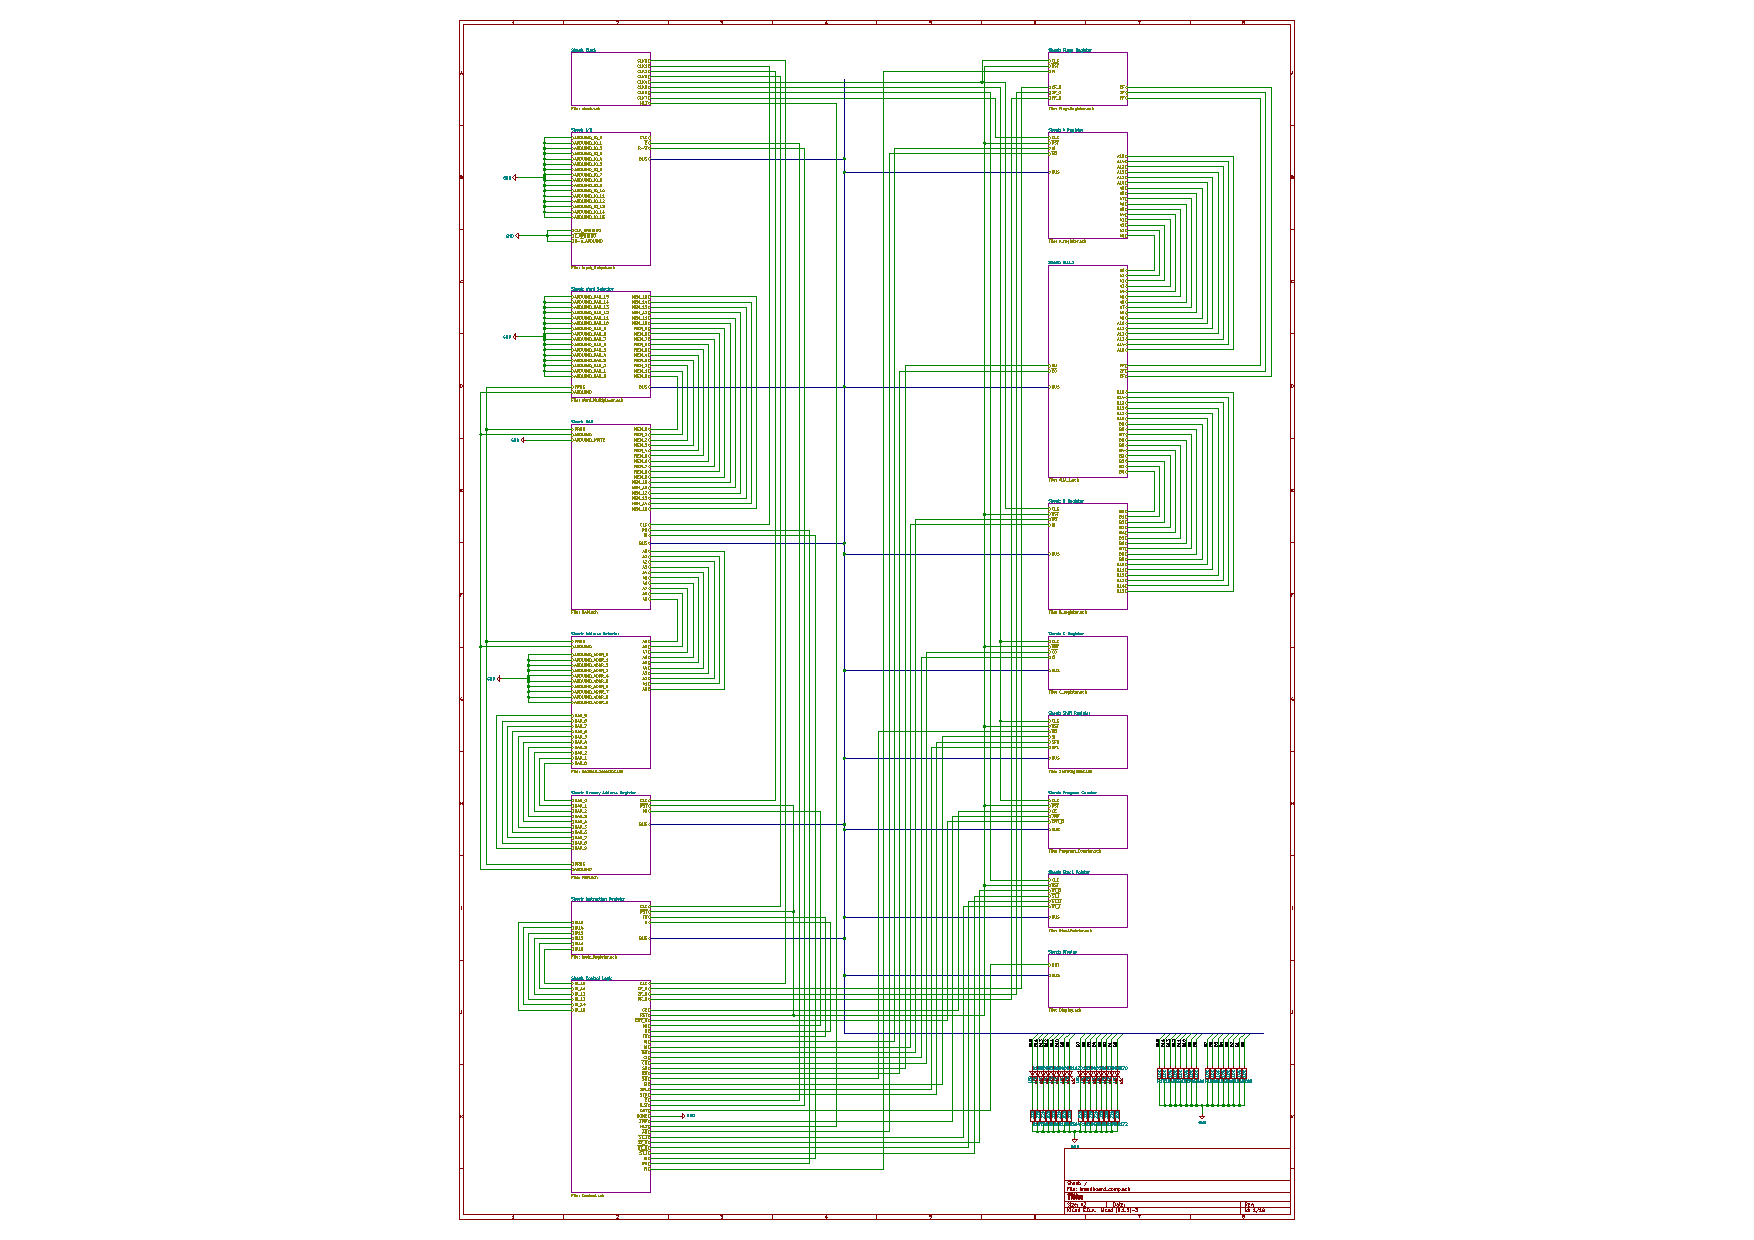
\includepdf[page={16}]{./pdf/kicad}

\chapter{Hardware Implementation}

\section{Hardware choices}
With the specification and design phase of the 16-bit breadboarc omputer now complete,

\chapter{Software Specification}
To transform the 16-bit breadoard computer from an exercise in logic design
into an advanced and rich learning meadium, a suite of feature-rich software
tools is needed.

\section{Main functionailty to be implemented}
The software for the breadboard computer should implement the following pieces
of high-level pieces of functionailty to be considered successfull:
\begin{itemize}
  \item \emph{Microcode definition and re-programming: } The computer needs the
  control logic EEPROM's \ref{control-logic} to be programmed with microcode. There
  should also be an accessible way to define and modify microcode.
  \item \emph{Assembler: } Given a set of instructions defined through microcode,
  there should be a way to write assembly instead of plain binaries and then assemble
  the code produced down to binaries
  \item \emph{Compiler: } Going up one more level of abstraction, one should be able
  to write a program in the WHILE programming language and then compile it down to
  either assembly or binaries directly.
  \item \emph{Programming arduino drivers: } Currently, the computer is programmed
  by setting the \emph{PROG} switch and then manually flipping dip switches on
  the word selector \ref{word-select} and the address selector \ref{addr-select}. This
  process is tedious, prone to mistakes and it can take a relativley long period of time
  to program a small number of instructions. Since an Arduino is connected to the word
  and address selectors, there should be a way to have th arduino program a binary produced
  by the assembler.
  \item \emph{I/O Arduino drivers: } While the I/O \ref{io} module has been built to its
  specification, it relies on the Arduino handling its read and write request. To achieve this,
  some driver software needs to be created.
\end{itemize}
The specification for each piece of software will be detailed in the following sections.

\section{Microcode Definition and Programming}
\subsection{Microcode format}
Currently, the only way to define instructions for the 16-bit breadboard computer is to write
binaries by hand, and then program them to the control logic EEPROMs. This is tedious and
prone to errors. There should exist a format through which instructions for the 16-bit breadboard
computer can be designed and stored. This format should be simple to read, understand, write and
change. The format should be high-level enough, so that the instruction designer doesn't have to
think about setting individual bits, while still being able to thik about which control signals
are set at which time step during which flag conditions. The format should specify the following
pieces of information regarding an instruction:
\begin{enumerate}
  \item Mnemonic (three-letter code)
  \item Opcode (6-bit number)
  \item Description (String)
  \item Whether the instruction requires an operand or not (boolean)
\end{enumerate}
Following this, each instruction should have associated to it at least one execution path.
This path should be dependant on the flag environment, but there should be at least one path
to serve as a default in all flag environments conditions which are not specified. An execution
path consists of a list of steps, each step detailing which control signals should be activated
at that particular time step.

 \subsection{Parsing and code generation}
 After a file declaring instructions conforming to the format described above is created, a script
 should exist which parses that file and generates 4 binaries from it, one for each EEPROM.

\section{Assembler}
Given a microcode generation tool, while it is now easy to write an \emph{instruction set} for the
16-bit breadboard computer, one would still have to write \emph{programs} in binary format. The
first level of abstraction away from writing binaries by hand should be an assembler.
The Assembler should fulfill the following requirements:
\begin{enumerate}
  \item  Dynamically recognize mnemonics based on a provided instruction definiton file
  \item  Recognise labels and replace them with memory locations
  \item  Recognise aliases and replace them accordingly
  \item  Recognise operands in decimal, hexadecimal and binary format
  \item Generate binaries based on an assembly source file and an instruction definiton file
\end{enumerate}

\section{Compiler}
To have a thorough understanding of the requirements and specifications for the \emph{WHILE}
language compiler, the language must be first presented and discussed.

\subsection{WHILE language}
The \emph{WHILE} language is a very simple Turing-complete programming language which is in syntax
very similar to pseudocode \ref{while-demo}.

\lstinputlisting[caption= \emph{WHILE} language Fibonacci program]{code/fib.while} \label{while-demo}

Some of the most important features of the \emph{WHILE} language are:
\begin{itemize}
  \item \emph{Limited types: } the language only has two types \emph{strings}, which can only be
  printed out, and \emph{integers}
  \item \emph{Simple statements: } the statements possible in the while language are \emph{while,
  if, assign, read, write}
  \item \emph{Restricted boolean and arithmetic expressions: } The while language an process data
  by executing instructions using simple arithmetic and boolean expressions. The allowed arithemtic
  operators are \emph{$+, -, *, /, \%$}. The allowed boolean operators are \emph{$\&\&, ||,  \leq, <, ==,
  >,  \geq$}
  \item \emph{Simplified I/O: } The \emph{WHILE} language uses the read and write statements to
  abstract the process of reading and writing data.
\end{itemize}

\subsection{Requirements}
Given the feature list of the \emph{WHILE} programming language described in the previous
section, a compiler should fulfill the following requirements:

\begin{itemize}
  \item Parse \emph{WHILE} source files
  \item Understand the underlying structure of the program
  \item Generate assembly code for a certain instruction set for the 16-bit breadboard computer
  which is built into the compiler.
\end{itemize}

\section{Programming Arduino driver}
In order to program the 16-bit breadboard computer with a binary generated by the assembler,
an Arduino driver coupled with a script to run on the main computer. The two pieces of software
should work in tandem to transmit a source file to the arduino and then on to the breadboard
computer. This should work as follows.

\subsection{Protocol specification}
\begin{enumerate}
  \item The Arduino is connected to the computer over USB
  \item The Arduino is manually reset
  \item The Arduino maintains an internal address counter, reset to 0
  \item The computer-side script reads a binary file and stores it in memory
  \item The computer sends the arduino two bytes at a time (two bytes form 1 breadboard
  computer instruction)
  \item The Arduino receives the 2 bytes and constructs a data word from them
  \item The Arduino programs the byte in the breadboard PC RAM at the address specified by its
  counter and then increments the counter
  \item The Arduino replies to the computer with a success message
  \item After the computer receives the success message, repeat from step 5
\end{enumerate}

\section{I/O Driver}
The I/O driver should work in a similar manner to the programming driver. It should allow the
the breadboard computer to interface with a personal computer by using the Arduino as an
information relay.

\subsection{Protocol Specification}
\begin{itemize}
  \item The Arduino is connected to the computer over USB
  \item The Arduino is manually reset
  \item The Arduino maintains an internal circular queue of 10 16-bit data words, which is
  initially reset to 0.
  \item If the computer sends data over to the Arduino, it should store that data at the end of
  the queue and update its queue pointer.
  \item If the breadboard computer triggers a read request, the Arduino should serve it a data
  word from the queue and then update its queue pointer.
  \item If the breadboard computer triggers a write request, the Arduino should read the data word
  found in the I/O module and then send it on to the main computer.
  \item The main computer should then display that data on the screen.
  \item At the start of the script on the main computer, a file should be provided which
  contains 10 numbers in either decimal, hexadecimal or binary format. This numbers should
  form the basis for the queue to be sent to the Arduino
\end{itemize}

\chapter{Software Design}

\section{Microcode format and programmer}

\subsection{Design Choices}

\paragraph{Language choice}
Given the fact that the microcode programmer will be tasked with processing
both text and binary files, \emph{Python} \cite{py} comes up as an obvious choice
for an implementation language. Python makes file manipulation and text
processing enjoyable instead of frustrating, as in many other languages, because it
requires essentially no boilerplate to achieve those goals. Moreover, Python is an
implements object-oriented philosophy, which will facilitate the creation of an internal
model for the instructions which are to be programmed. The syntax is also light weight,
concise and understandable, which makes \emph{Python} a good choice for a scripting
language as well. This is important because the microcode programmer will be a command-line
script.

\paragraph{Microcode Instruction Format}
Given the specification for a simple to learn and used format for declaring
microcode instructions, two possiblities come to mind:

\paragraph{Language specific} One approach would be to create classes for the
microcode instructions in some object-oriented programming language. This way,
a user who is familiar with the language could easily create multiple objects which
are instantiations of that particular class. After the user has created the class
instances, he could run a script to generate microcode instructions from them.
Since the implementation language chosen is \emph{Python}, Instructions would be
represented as Python objects.

\paragraph{Language agnostic} Another approach would be to make use of a format
which doesn't depend on a specific programming language. The main advantage of this
approach would that someone who isn't familiar with the implementation language
could use the tool efectivley. This would also mean that the programmer would
have to contain a parser for this format, separate from the parser of the implementation
language. A good choice of format for such an approach might be \emph{YAML} \cite{yaml}.
\emph{YAML Ain't Markup Language} (recursive definition), is a data serialization language
designed around the main goal of being human-readable \cite{yaml}. As such, it poses itself
as a great choice for the microcode definiton format, as it is so simple that one
does not have to be familiar with it to quickly undestand it and use it. Both approaches
towards formatting microcode instructions should be implemented.

\subsection{Programmer design}
Given a file in either of the two formats discussed in the previous section, the programmer
should follow the following broad steps
\begin{enumerate}
  \item If provided a Python source file, parse it and extract the instruction objects
  \item If provided a YAML file, parse it and then convert the YAML objects to Python instruction
  objects
  \item Generate 4 bytearrays containing zero bytes. The bytearrays should be of the size of the
  memory arrays of the control logic EEPROMs
  \item For each instruction, for each flag environment, for each step:
  \item Concatenate the binary formatting of the opcode, flag environment and time step
  \item Interpret the resulting string as a binary number and convert it to an integer
  \item Use the resulting integer as a pointer to write
  the control signal bytes of that timestep to the right place in the bytearrays
  \item If no control signal sequence is provided for a certain flag environment, use the default
  one
  \item Write the resulting bytearrays to files
\end{enumerate}


\section{Assembler}

\subsection{Design choices} \label{asm-des}

\paragraph{Language} For the assembler for the 16-bit computer the choice was made to
use a different language then the one used for the microcode programmer, namely \emph{Scala}
\cite{scala}. \emph{Scala} is a modern multi-faceted multi-paradigm all-purpose built on top
of the Java ecosystem. \emph{Scala} is large-scale widley-used and fully-featured to such an
extent that it would be infeasable to cover all of its features in this report. However, noting
the most important language features will shed light onto why it poses itself as a great tool
for implementing assemblers and compilers:

\paragraph{Functional programming}
Scala has all the functionality needed to implement programs and scripts following a functional
paradigm. This feature lends itself to the advantage in the task of implementing an assembler
and compiler because of the natural tendency to solve assembling and compiling tasks using
recursive functions. Functional programming encourages and simplifies the creation of recursive
functions.

\paragraph{Java Ecosystem}
Since \emph{Scala} is built on top of \emph{Java} \cite{java}, the entire \emph{Java Ecosystem}
is a subset of \emph{Scala}. As such, \emph{Scala} doesn't confine the developer to functional programming, allowing great freedom in mixing and matching styles and paradigms.

\paragraph{Robust yet Concise Typesystem}
\emph{Scala} comes with all the benefits of the \emph{Java} typesystem, including stron typing,
type checks, object oriented approach, subclasses, abstract classes and many other, while at the
same time not having the same downsides. The main advantage of the \emph{Scala} typesystem is the
fact that it requires significantly less boilerplate than its \emph{Java} counterpart. This
feature is useful given the inherent need of compilers and assemblers generally to create many
internal data structures to faciliate the transformation of source code from one format to the
next.


\paragraph{Dynamic and flexible Syntax}
The \emph{Scala} syntax is concise and understandable, similar to Python in many ways. Unlike
Python syntax, it has some key advantages. It doesn't rely on indentation to determine scope,
which can be a source of frustration allthough it makes code much more readable and it gives
the user the option to extend and augment the syntax using implicit definitions. This makes
the life of the assembler and compiler designer easier by allowing him to write shortcuts in
places were repetitive tasks are undertaken.

\paragraph{YAML Parser}
Since the assembler will have to be aware of any changes in instruction set defined by the user
for the 16-bit breadboard computer, the need for a YAML parser arrises. This parser will be used
to process the same list of instructions used by the microcode programmer and then collect a list
of mnemonics. Using this list, the parser can determin if the assembly source file conforms to
that particular instruction set.

\subsection{Assembler Design}
The Assembler will be built around a two-module design. A \emph{Lexer} and a \emph{Code
generator}.

\paragraph{Lexer}
The task of the \emph{Lexer} is to transform the contents of an assembly file, essentially a
simple string, into a list of tokens. Then, the \emph{Lexer} can pass on the token list to the
\emph{Code generator}. The \emph{Lexer} uses \emph{regular expressions} to read the input string
and break it down into tokens. When a piece of the input string matches a particular token
pattern, an instance of that token is created with that specific piece and then added to the
list. Then the \emph{Lexer} continues to process the remaining input string. Besides this, the
\emph{Lexer} also has the task of eliminating whitespace and comments from the token list,
as these play no role in code generation. The lexer contains a custom-built regular expression
engine built around the concept of \emph{regular expression derivates}. This alternate way
to think about and implement regular expressions is taught by \emph{Dr. Christian Urban} in the
\textbf{6CCS3CFL} course\cite{6ccs3cfl}. The use of derivative regular expressions significantly
improves performance in certain edge cases. When a match is found, an injection function is used
to rebuild a ``value'' from the derivative which points towards which token has matched.

\paragraph{Code generator}
The \emph{code generator} receives the list of tokens from the \emph{Lexer} and then does further
processing on it. Since assembly doesn't have a complex syntax or structure, there is no need
for a parses. The assembler completes the following steps to fullfil its task:
\begin{enumerate}
  \item Alias extraction
  \item Subroutine ordering
  \item Subroutine separation
  \item Reference solving
  \item Instruction decoding
\end{enumerate}
Once these steps are completed, the code generator is able to generate a bytearray and write a
binary file to disk.


\section{Compiler}
\subsection{Design Choices}
\paragraph{Language}
Since the Compiler and the Assembler share a significant amount of structure and code, the choice was made to also
use \emph{Scala} for the compiler. The reasons for this choice have been stated in the Assembler design choices
section \ref{asm-des}.
\paragraph{Structure}
The compiler has a similar structure to the assembler. It also has a \emph{Lexer} and a \emph{Code Generator}.
The main difference is the presence of a third module, namely the \emph{Parser}. The \emph{Parser} sits between
the \emph{Lexer} and the \emph{Code Generator} and is tasked with generating an \emph{Abstract Syntax Tree} from
the list of tokens.
\subsection{Compiler Design}
\paragraph{Lexer} The compiler \emph{Lexer} follows the same design pattern as the one used for the assembler.
The main difference between the two is that they use different regular expressions to parse the input string.

\paragraph{Parser} The \emph{Parser} has the task of taking the token list, which has no structure except for the
total ordering imposed onto it and then turn it into a \emph{Abstract Syntax Tree}, or \emph{AST} for short. An
\emph{AST} encapsulates the internal structure of a program, like for example nested loops, if-else branches and the
order of operations in an arithmetic expression. The \emph{Parser} of the compiler is based on a parsing philosophy
called ``parser combinators'', which is also taught by \emph{Dr. Christian Urban} in the \textbf{6CCS3CFL} module
\cite{6ccs3cfl}. Parser combinators work by defining simple as objects which try to parse as much of the input tokens
as possible and then return the amount they could parse, as well as the remaining part of the input which they
couldn't process. By taking multiple simple parsers and \emph{combining} them (hence the name), a more complex parser
can be created. Their nature is to return a set of pairs of processed and unprocessesed input. This way,
the next parser in line can try to parse based on all the different ways the previous parsers parsed.
When the infrastructure has been set up, writing parser combinators for a language can be as simple as declaring
the grammar of that particular language. Parser combinators make use of \emph{lazy evaluation}
which is a mode in which arguments are only evaluated at the last possible moment in time.

\paragraph{Code generator}
The code generation stage for the Compiler is simplified, since most of the processing has been completed by the
\emph{Parser}. In this case, the \emph{Code generator} has to traverse an abstract syntax tree recursivley and then
map its elements to chunks of code from the target language, in this case 16-bit breadboard computer assembly.


\section{Programming and I/O Arduino Drivers}
\subsection{Design choices}

\paragraph{Language} For the design of the programming and I/O Arduino drivers, \emph{Python} was chosen for the
script on the computer side and \emph{C} was chosen for the Arduino script. \emph{Python} is a great scripting
language and it handles file I/O, both binary and text, in an elegant manner. So it presented itself as a good
choice for the scripts running on the computer. \emph{C} was chosen for the Arduino scripts because it is the only
language supported by the Arduino Integrated Development Environment \cite{arduino_ide}.

\subsection{Script Design}
The scripts for running the Arduinos do not offer much in term of design depth, since they are relativley short
and simple. What is notable is the need to use interrupts to interface with the breadboard computer and the use of
the serial port to communicate to the computer. The Arduinos also make extensive use of bitshifting and bit
extraction to convert data from the internal datatypes to voltages on multiple pins and pin voltages to datatypes.

\chapter{Software Implementation}
This chapter details the process through which the software previously designed
was implemented. Additionally, tools and libraries used were discussed.


\section{Implementation Process}
The different software tool were developed in sequence. This was because
each tool was dependent on the previous to work. After each short development
interation. Where possible, the software was tested against either the phyisical implementation
of the 16-bit breadboard computer or against test files.

\section{Libraries used}
Besides the standard libraries of both \emph{Python} and \emph{Scala}, as well as
the standard \emph{C++} functions provied by the \emph{Arduino IDE}, the following libraries
were also used to simplify and expedite the implementation process:
\paragraph{PyYAML} \cite{pyyaml} PyYAML provides a YAML parser for Python. In this case it was
used on the microcoed generator to parse instructions in YAML format. PyYAML converts a YAML
file into a python object consisting of lists, dictionaries and primitives.

\paragraph{PySerial} \cite{pyserial} PYSerial was used to implement the communication link
between the computer and the two Arduinos.

\paragraph{moultingYAML} \cite{moultingyaml} MoultingYAML is a YAML parser for Scala. It works
more subtly than PyYAML, as it allows the user to specify a \emph{Protocol} with which to
parse a YAML file directly into a user-defined custom Scala object. It was used in the
assembler to parse instruction set files.

\paragraph{Scala Binary Files pattern} \cite{scala-bin} This gist was used as an inspiration
source for using Scala to write binary files to disk.

\section{Source-code basis}
The basis of the source code for both the assembler and the compiler is the fouth coursework
of the \textbf{6CCS3CFL} course taught by \emph{Dr. Christian Urban} \cite{6ccs3cfl}.

\section{Tools used}

\paragraph{Build Tools} Given the simplicity of the scripts, no build tools were used for the
implementation of the microcode programmer and the two arduino drivers. For the implementation
of the assembler and compiler, \emph{Scala Build Tools} (sbt) was used \cite{sbt}. Sbt handled
dependecies, installation of scala, the interactive interpreter and the running of the script.

\paragraph{EEPROM programming} The microcode generator creates binary files, but does not
burn them to the EEPROMs, for this, a separate software and hardware solution was used.
The \emph{TL866 II Plus} \cite{eepromg_prog} EEPROM programmer with its accompanying software
\emph{XgPro} \cite{xgpro}. This programmer is widley adopted and offers compatibility with a wide rage
of chips, including the \emph{AT28C64B} EEPROM \cite{at28c64b}. The software was simply used to
interface with the programmer, read .bin files and program them into the chips. No other functionality
provided by the software was used.

\section{Source code Listing}
A complete listing of the source code produced is availalble in the \emph{Appendix}.

\chapter{Software Testing}

\section{Testing Methodology}
Since each piece of software was dependant on the software before it, each new tool
developed was tested during and immediatley after its development process. Taken
the relativley reduced complexity and size of each of the tools created, the decision
was made to skip \emph{unit testing} and only conduct \emph{integration testing}.

\section{Microcode programmer}
The microcode programmer was tested by writing an instrution set consisting of only one instruction
in both Python and YAML format and then generating binaries from that source. Then, the resulting
binaries were checked by hand to ensure that the right byte sequences were generated. After the
creation of richer instruction set, random samples were selected from the instruction set source
and then the binaries were checked for those particular instructions. \\
The microcode generator passed all tests successfully.

\section{Assembler and Compiler}

\paragraph{Assembler}
The Assembler was tested with multiple source files designed to incorporate all the features it
had specified: mnemonics, operators, aliases, labels. All files were assembled down to binaries
correctly.

\paragraph{Compiler}
Similarly, the compiler was checked against three WHILE language source files, two of which were used
as test files in the \textbf{6CCS3CFL} course thaught by \emph{Dr. Christian Urban} \cite{6ccs3cfl}.
All files were correctly compiled down to assembly.

\section{Arduino drivers}
\paragraph{Programming driver}
The programming driver was tested by generating zero-byte binaries, one-byte bineries and multiple
binaries with repeating patterns of bytes and then using the computer script and the driver software
to program the 16-bit breadboard computer. Then, using the manual programming mode to set the address
and tying the \emph{RO} (RAM-Out) signal high, random samples accross the entire memory space of the
computer were checked. All samples matched the expected bytes.

\paragraph{I/O driver}
The I/O driver was checked by having loading in sequences of \emph{LAI - IRA} instructions (Load A
immediate and I/O read A) with specific bit sequences as the operand for the \emph{LAI} instructions,
and then checking if the correct output was displayed back on the computer. To test the I/O reads,
multiple\emph{IWA} instructions (I/O write A) were executed together with specific queue values. It
was then checked if the expected value had been read into the A register. Unfortunatly,
at the time of writing, the I/O Arduino behaves iratically, only sometimes writing and reading from the
I/O module. It is unclear whether this is due to the software, the hardware or a combination of both.
This will be discussed as a point of imporvement in a following section.



\chapter{Evaluation}
To evaluate the success of the 16-bit breadboard computer architecture project, a parallel between
the goals set out at the start of the report and what was achieved in practice has to be drawn and
each success criterion has to be considered.

\section{Achieved Objectives}

\subsection{Analysis objectives}
\begin{enumerate}
  \item \emph{Computer architecture analysis:} this goal was successfully met in the background
  \ref{background} section of the report, where computer architecture, processor design,
  microarchitecture and processor component design were presented and discussed
  \item \emph{Analysis of the computer designed and built by Ben Eater: } \cite{eater2019breadboard}
  this objective was also successfully achieved in the background section of the report
  \ref{background}.
\end{enumerate}

\subsection{Hardware objectives}
\begin{enumerate}
  \item \emph{16 bit word length} : achieved both in design and implementation
  \item \emph{appropiatley sized memory space} : achieved both in design and implementation
  \item \emph{memory read/write capability} : achieved both in design and implementation
  \item \emph{capability to decode and execute instructions sequentially} : achieved both in design and implementation
  \item \emph{program counter alteration (jumps)} : achieved both in design and implementation
  \item \emph{I/O functionality} : This goal has not been fully achieved at the time of writing
  \item \emph{hardware-implemented ability to perform basic arithmetical operations} : achieved both in design and implementation
  \item \emph{simple branching} : achieved both in design and implementation
  \item \emph{variable speed clock} : achieved both in design and implementation
  \item \emph{single step clock function} achieved both in design and implementation
\end{enumerate}

\subsection{Software objectives}
\begin{enumerate}
  \item \emph{microcode generation tool} - completed successfully
  \item \emph{adequate microcode for the control mechanisms} - completed successfully
  \item \emph{assembly mnemonics} - completed successfully
  \item \emph{assembler package to turn assembly files into binaries} - completed successfully
  \item \emph{compiler for the WHILE-language to breadboard computer binaries} - partially completed.
  Discussed in the \emph{Unmet Objective} section \ref{unmet}
  \item \emph{Arduino driver software} - partially completed.
  Discussed in the \emph{Unmet Objective} section \ref{unmet}
\end{enumerate}

\section{Unmet Objectives} \label{unmet}
Both the hardware and software produced meet most of their set out objectives. That being said, a few
objectives have not been achieved fully. These will be discussed in this section of the report.

\subsection{I/O Issues}
While both the software and the hardware for the I/O module has been designed and built, it fails
to operate consistently. This makes deugging challenging, since there is no clear point of failure.
That being said, two theories have the largest likelyhood of successfully identifying the root cause.

\paragraph{Voltge spikes produced by the EEPROMs} After the incidient concerning the undefined
behaviour of the EEPROMs during an address change, this possibility first came to mind as a potential
source for the issues. The patch which was tried immediately was the insertion of RC-network filters
on the control signals which command the I/O module and the A register. This did not solve the abnormal
behaviour, but only filtering either one or the other module at one time was tried, not both at the
same time.

\paragraph{Code timing issues} It is possible that due to the fact that all events happend in the
computer at the same time, namely on the rising edge of the clock pulse, the interrupt triggered
on the arduino immediately reads the bus contents while they are still switching. This theory
is hard to prove though, since ISR (Interrupt Service Routine) of the Arduino has to be as short and
without delay calls.

\subsection{Compiler}
While the \emph{WHILE} language compiler works as specified and produced valid assembly files,
two features of the \emph{WHILE} language are missing from the implementation.

\paragraph{Strings} The \emph{WHILE} language has the option to print out strings of characters
to the screen. This feature has not been implemented in the Compiler for the language. That being
said, strings are not a part of the objectives set out for the hardware implementation, so there is
nothing to compile to. As such, it is debatable whether this constiutes an unmet objective.

\paragraph{Operators} Two arithmetical operators are missing from the \emph{WHILE} language compiler,
\emph{/ (Division)} and \emph{\% (the modulo operator)}.

\section{General Objective}
Given the main goal to create a hardware architecture which is both practically implementable
and easy to understand to a low level, as well as the creation of a suite of software tools to
accompany it and based on the list of achieved objectives, it is safe to say that the general objective
has been successfully achieved. The 16-bit breadboard computer is a physically implemented, it is
easy to understand how it functions and it can act as a great taching and learning medium for
computer architecture, design, implementation, general low-level programming as well as compilers and
assemblers.

\chapter{Legal, Social, Ethical and Professional Issues and application of the BCS Code of Conduct}

\section{Legal, Social, Ethical and Professional Issues}

Taken into account the nature of this project and the way it has been conducted,
Legal, Social, Ethical and Professional Issues were unlikley to arrise. That being
said, it is important to go over each field separatley and show that no issues pertaining
to that field have appeard.

\begin{itemize}
  \item \emph{Legal issues: } The project did not pose any legal issues. There was no need
  to contact third parties, gain access to sensitive or classified information or any other
  activity which chould have created legal issues.
  \item \emph{Social or Ethical issues: } The project did not pose any social or ethical issues.
  There was no need to gather personal data, conduct surveys, create control groups or anything
  similar which could have affected the project and create social or ethical issues.
  \item \emph{Professional issues: } one professional issue presented itself early on in the
  project. As the project had a significant hardware component, the need to purchase the hardware
  became aparrent. The issue at hand was to determine who would fund the hardware needed for the
  project. After careful consideration, the decision was made to fund the project using personal funds
  so as to not have to be dependant on any other body or entity.
\end{itemize}


\section{Application of the BCS Code of Conduct}
The British Computer Society Code of Conduct \cite{bcs} applies to the project and, as such, the
project abides by this code of conduct. The main section where it is visible that this report aims to
abide by the BCS Code of Conduct is the ``Duty to the Profession'' section, point ``f'', as  well as
the ``Duty to the Profession'' interpretation. They state that a fellow abiding by the BCS Code
of Conduct shall ``encourage and support fellow members in their professional development'' and ``share
knowledge and understanding of IT and support inclusion of every sector of society.''. One of the main
goals of the project is to make computer architecture and design easier to approach from any
potential background and learn more about how computers work at a very low level. This is a reflection
of the directives cited above.

\chapter{Next Steps and Conclusions}

\section{Next Steps}
While a significant amount of work has been done towards making the 16-bit breadboard
computer a polished project, there are many goals which can still be achieved if the
project were to be continued.
\begin{itemize}
  \item \emph{I/O Troubleshooting:} The I/O module is not fully functional. A first step
  towards improving the 16-bit breadboard computer would be to ensure that this module
  works as specified as well.
  \item \emph{More Complex Instruction Set: } currently, the instruction set defined for the 16-bit
  breadboard computer is mostly composed of instructions which execute very simple tasks, like moving
  a value between registers or adding up two numbers. It might be interesting to see how the
  functions of the computer, as well as the design of the assembler and compiler would change given
  a minimal instruction set and an instruction set designed to be as complex as possible.
  \item \emph{Compiler optimizations: } The Compiler produced in this project  achieves the goal
  of compiling \emph{WHILE} language sources down to assembly, but it doesn't apply any compiler
  optimizations. For example, the multiply subroutine, which currently essentially just adds the
  multipliand with itself as many times as the multiplier, could be replaced with a shift-add
  subroutine.
  \item \emph{Added functionality } currently, the computer handles only unsigned integers. It would be
  interesting to see if it is possible to extend to signed integers, characters, strings and arrays
  without adding any more hardware.
  \item \emph{More complex programs: } Another potential goal would be to test the 16-bit breadboard
  computer with more complex programs. A good starting point might be sorting algorithms.
  \item \emph{LLVM integration: } The LLVM suite of programs has at its core the \emph{LLVM IR}
  \cite{llvm}, or \emph{Intermediate representation} This low-level language is designed to sit between
  hardware and  programming languages and allows programming language designers to compile their
  language down to the IR and then run on any hardware which implements a compiler from the IR to their
  particular instruction set. It would be interesting to see if it possible to write a compiler from
  a subset of the IR and then use this abstract language interface to run programs written in modern
  high-level languages on the 16-bit breadboard computer.
\end{itemize}


\section{Conclusion}
The 16-bit breadboard computer architecture project ended up being an outstanding learning experience
for learning about computer architecture, processor design, hardware design and low level software
design and implementation. The end product is something that can complete many of the tasks that
modern computers complete, while still being simple and understandable down to a very low level of
abstraction. This report can serve as a guide for anyone who might want to attempt a similar
undertaking or just focus on learning about computer architecture. While offering few practical
advantages, such a computer can be of significant use in modern life, not just as a teaching medium,
but also as a way for a software engineer to become more connected with the hardware he uses in his
day to day activities and to have a better grasp of the capabilities and limitations of the tools
at his disposal.



%%%%%%%%%%%%%%%%%%%%%%%%%%%%%%%%%
% References
%%%%%%%%%%%%%%%%%%%%%%%%%%%%%%%%%
\bibliographystyle{plain}
\bibliography{mybib}
\addcontentsline{toc}{section}{Bibliography}

%%%%%%%%%%%%%%%%%%%%%%%%%%%%%%%%%
% Appendices
%%%%%%%%%%%%%%%%%%%%%%%%%%%%%%%%%
% \appendix
% \include{Appendices/appendix}
% \chapter{User Guide}
\section{Instructions}
You must provide an adequate user guide for your software. The guide should provide easily understood instructions on how to use your software. A particularly useful approach is to treat the user guide as a walk-through of a typical session, or set of sessions, which collectively display all of the features of your package. Technical details of how the package works are rarely required. Keep the guide concise and simple. The extensive use of diagrams, illustrating the package in action, can often be particularly helpful. The user guide is sometimes included as a chapter in the main body of the report, but is often better included in an appendix to the main report.

% \chapter{Source Code}
\section{Instructions}
Complete source code listings must be submitted as an appendix to the report. The project source codes are usually spread out over several files/units. You should try to help the reader to navigate through your source code by providing a ``table of contents'' (titles of these files/units and one line descriptions). The first page of the program listings folder must contain the following statement certifying the work as your own: ``I verify that I am the sole author of the programs contained in this folder, except where explicitly stated to the contrary''. Your (typed) signature and the date should follow this statement.

All work on programs must stop once the code is submitted to KEATS. You are required to keep safely several copies of this version of the program and you must use one of these copies in the project examination. Your examiners may ask to see the last-modified dates of your program files, and may ask you to demonstrate that the program files you use in the project examination are identical to the program files you have uploaded to KEATS. Any attempt to demonstrate code that is not included in your submitted source listings is an attempt to cheat; any such attempt will be reported to the KCL Misconduct Committee.

\textbf{You may find it easier to firstly generate a PDF of your source code using a text editor and then merge it to the end of your report. There are many free tools available that allow you to merge PDF files.}


\end{document}
